% Copyright (c) 2008-2009 solvethis
% Copyright (c) 2010-2016,2018-2019,2021 Casper Ti. Vector
% Copyright (c) 2021 Kurapica
% Copyright (c) 2021 iofu728
% Overleaf version.

%*********************************************************************
% iofu728-pkuthss: 北京大学研究生学位论文模板
% 2021/06/09 v1.0.0
%
% 重要提示：
%   1. 当前overleaf版符合2021研究生学位论文要求，可通过图书馆审核
%   2. 当前版本基于pkuthss v1.9.1
%   3. 请使用UTF-8编码，XeLaTeX方式编译
%   4. 请仔细阅读用户文档
%   5. 修改、使用、发布本文档类请务必遵循LaTeX Project Public License和知识共享4.0
%   6. 如有疑问github/iofu728/pkuthss上提问或联系作者@iofu728
%*********************************************************************

\documentclass[fontset=fandol,ugly]{pkuthss}
  % 学位论文模式  ugly    (默认打开，请保留)
  % 盲审模式      blind   (默认关闭)
  % 字体库        fontset
  %   auto | windows | windows@overleaf | mac | fandol | ubuntu | none
  % windows*, mac为商业字体，如需使用请遵循相应版权协议(默认下overleaf中不可用)
  % fandol与windows效果相近，但字符库偏少，推荐使用(默认);
  % ubuntu字体效果偏差较大; 设为none时需自行配置字体集;

\usepackage[backend=biber,style=gb7714-2015]{biblatex}
  % 参考文献遵循GB/T 7714-2015标准，使用biblatex-gb7714-2015 宏包。
  % 此处使用顺序编码制，如使用著者-出版年制则更改为b7714-2015ay。

% 给adamoe的字体用 \def\AdaMoE{\raisebox{0.05ex}{\scalebox{0.96}{$\mathbf{\mathcal{A}}$}}\textit{da}\raisebox{0.04ex}{\textsc{\scalebox{0.85}{MoE}}}\xspace}

\usepackage{graphicx}
\usepackage{xspace}
\usepackage{amsmath}

% 示例文档用包和设定，该段均可移除.
\usepackage{enumitem,fancyvrb}
\usepackage{booktabs,multirow,longtable,makecell} % 表格相关
\RecustomVerbatimEnvironment{Verbatim}{Verbatim}{frame = single, tabsize = 4, fontsize=\footnotesize}
\renewcommand{\v}[1]{\boldsymbol{#1}}
\newcommand\pkg[1]{\textsf{#1}}

% 伪代码
\usepackage[ruled]{algorithm2e}

% 参考文献边距字体
\setlength{\bibitemsep}{3bp}
\renewcommand*{\bibfont}{\zihao{5}\linespread{1.27}\selectfont}

\pkuthssinfo{
	cthesisname = {博士研究生综合考试},
 	thesiscover = {博士研究生综合考试},
	ethesisname = {PhD Qualification Exam},
	ctitle = {混合专家模型架构设计\\与训练综述},
	etitle = {A survey on Architecture and Training of Mixture of Experts},
	cauthor = {王乐安}, eauthor = {Lean Wang},
	studentid = {2301111960},
	% 具体时间以教务为准，初稿3月，送审4月，答辩5月，最终6月。
	date = {\zhdigits{2025}\ \ 年\ \ \zhnumber{10}\ \ 月},
	school = {计算机学院},
	cmajor = {计算机软件与理论}, emajor = {XXXX},
	direction = {自然语言理解},
	mentorlines = {1}, % 导师个数
	% 副教授 A.P. 讲师 Lec.
	cmentor = {孙栩\ \ 研究员}, ementor = {Prof.\ Xu Sun},
	ckeywords = {A，B，C，D},
	ekeywords = {A,B,C,D},
	% 盲审模式参数, 需在documentclass增加blind
	blindid = {XXXXXXXXX}, discipline = {XXXX}
}
\addbibresource{ref.bib}

\DeclareMathAlphabet{\mathcal}{OMS}{cmsy}{m}{n}
\let\mathbb\relax % remove the definition by unicode-math
\DeclareMathAlphabet{\mathbb}{U}{msb}{m}{n}


% token 标记

\begin{document}
	\frontmatter
	\pagestyle{empty}
	\maketitle
	% \cleardoublepage
	% 需替换门户版权声明pdf
	% \include{chap/copy}

	\cleardoublepage
	\pagestyle{plain}
	\setcounter{page}{0}
	\pagenumbering{Roman}
	% \begin{cabstract}
	中文摘要部分...
\end{cabstract}

\begin{eabstract}
    英文摘要部分...
\end{eabstract}

% vim:ts=4:sw=4

	\tableofcontents
	% 如有需要使用主要符号对照表
	% \include{chap/deno}

	\mainmatter
	\chapter{引论}
\label{chap:introduction}

近年来，以Transformer架构为基础的大语言模型（Large Language Models, LLMs）取得了革命性的进展，在自然语言处理乃至更广泛的人工智能领域引发了深刻的范式变革。从BERT\cite{Devlin2019BERTPO}、GPT\cite{Radford2018ImprovingLU}系列到如今数千亿甚至万亿参数的巨型模型，LLMs通过在海量数据上进行预训练，展现出了前所未有的语言理解、生成乃至推理能力，并在多种下游任务中取得了卓越表现。

这种成功的核心驱动力之一是“规模定律”（Scaling Laws），即随着模型参数量、数据量和计算量的增加，模型的性能也会可预测地持续提升\cite{Kaplan2020ScalingLF}。遵循这一规律，学术界和工业界竞相投入巨大的资源来训练更大、更强的“稠密”（Dense）模型。然而，这种依靠堆砌资源、暴力美学式的发展路径正面临日益严峻的挑战。训练一个拥有数千亿参数的稠密模型，需要惊人的计算资源（数千乃至数万个GPU/TPU）。例如，GPT-3\cite{Brown2020LanguageMA}（1750亿参数）的单次训练成本高达数百万美元\cite{lambdaai2020demystifyinggpt3}。对应的，其推理成本也居高不下，大大影响了部署此类模型的经济效益\cite{Erdil2025InferenceEO}。这种高昂的成本不仅限制了模型的迭代速度，也使得广大研究者和中小型机构难以参与到前沿模型的研发中。因此，“稠密”的巨型模型已非长久之计。学术界和工业界开始积极探索新的路径，以期在维持甚至超越现有模型性能的同时，显著提升计算效率。在这一背景下，“稀疏化”（Sparsity）成为了一个极具吸引力的研究方向。

混合专家模型（Mixture-of-Experts, MoE）\cite{Jacobs1991AdaptiveMO}作为一种实现模型稀疏化的有效途径，近年来重新焕发了强大的生命力。MoE的核心思想根植于“分而治之”的理念，其历史可以追溯到上世纪90年代的早期神经网络研究 \cite{Jacobs1991AdaptiveMO,Jordan1993HierarchicalMO}。其基本框架是，将一个庞大的模型拆分为多个相对较小的、功能各异的“专家”子网络，并通过一个“门控网络”（Gating Network）或“路由器”（Router）来决定每个输入（例如一个token）应该由哪些专家来处理，并将专家的输出加权合并，形成最终的输出。

与稠密模型在处理每个输入时都激活全部参数不同，现代MoE模型采用\textbf{条件计算}（Conditional Computation）机制，即每次只激活一小部分专家网络。这意味着模型的总参数量可以非常庞大（从而拥有巨大的模型容量），但实际的计算量却只与被激活的少数专家相关，从而在大幅增加模型规模的同时，保持了计算成本的相对恒定\cite{Shazeer2017OutrageouslyLN}。

将混合专家模型架构与Transformer结合，是近年来最重要的突破之一。通过将Transformer中的前馈神经网络层（Feed-Forward Network, FFN）替换为MoE层，研究者们成功地将模型参数扩展到了万亿级别，如谷歌的GShard\cite{Lepikhin2020GShardSG}和Switch Transformer\cite{Fedus2021SwitchTS}。普遍认为，当前的一线闭源模型GPT-4\cite{Achiam2023GPT4TR}、Claude Opus 4\cite{anthropic2024claude4}和Grok 4\cite{xai2025grok4}有很大可能均使用了混合专家模型架构；特别地，谷歌的顶尖模型Gemini 2.5 Pro\cite{comanici2025gemini25pushingfrontier}声明了自己使用了混合专家模型架构。近期，开源社区也涌现出如Mixtral 8x7B\cite{Jiang2024MixtralOE}、DeepSeek-V3\cite{DeepSeekAI2024DeepSeekV3TR}、Kimi K2\cite{Bai2025KimiKO}等一系列较高性能的混合专家模型，极大地推动了该技术的发展和普及，大大促进了开源高性能模型的商业化部署。

本文旨在全面回顾与总结当前面向大规模预训练模型的混合专家模型的研究进展。我们将系统性地梳理混合专家模型的关键技术、主流架构、训练策略以及相关的分析工作。特别地，在此基础上，本文将进一步讨论我们在混合专家模型负载均衡策略方面的个人研究进展，即\textbf{一种无辅助损失的负载均衡策略（An Auxiliary-Loss-Free Load Balancing Strategy for Mixture-of-Experts）}\cite{Wang2024AuxiliaryLossFreeLB}。通过本综述，我们期望能够为相关领域的研究人员乃至其他领域的感兴趣者提供一个对混合专家模型的全局认识，以及在特定细分方向（负载均衡）的深入认知。


% not finished

本文的后续章节按照如下方式组织：
\begin{itemize}
    \item 第二章将介绍理解混合专家模型所必需的背景知识，主要包括作为现代大语言模型基石的 Transformer 架构、混合专家模型的基本原理与核心组件，以及预训练大语言模型的演进脉络。
    \item 第三章将深入探讨经典的混合专家模型架构与训练方法，重点梳理其经典的稀疏架构、Top-k 路由算法的多种变体与优化，并详细分析混合专家模型训练中的核心挑战——负载均衡问题及其主流解决策略。
    \item 第四章将综述混合专家模型领域的多种前沿变种，介绍包括专家选择路由（Expert Choice Routing）在内的非 Top-K 路由机制，以及将混合专家思想从前馈网络扩展至注意力机制、模型深度等其他维度的创新架构。
    \item 第五章将详细阐述本人的个人研究进展，即我们提出的“无辅助损失均衡（Auxiliary-Loss-Free Balancing）”负载均衡策略。本章将从动机、算法设计、实验结果等多个方面全面介绍该方法。这一方法旨在解决传统辅助损失带来的性能与均衡之间的困境。
\end{itemize}
        \chapter{背景介绍}
\label{chap:background}

随着大规模预训练语言模型（Large Language Models, LLMs）在自然语言处理及更广泛的人工智能领域取得巨大成功，模型规模的持续扩张成为提升性能的关键驱动力。然而，由此带来的计算资源和训练成本的指数级增长，促使学术界和工业界探索更高效的模型架构。混合专家模型（Mixture-of-Experts, MoE）作为一种实现条件计算（conditional computation）的有效范式，能够在不显著增加计算量的前提下，将模型参数量扩展到数万亿级别，成为构建前沿大语言模型的核心技术之一。本章将介绍理解MoE模型所必需的背景知识，主要包括作为现代大语言模型基石的Transformer架构、混合专家模型的基本原理，以及预训练大语言模型的演进脉络。

\section{Transformer 架构回顾}

自Vaswani等人在2017年提出以来，Transformer架构凭借其核心的自注意力机制（Self-Attention Mechanism），彻底改变了序列到序列（sequence-to-sequence）任务的处理方式，并迅速成为自然语言处理领域的标准架构 \cite{Vaswani2017AttentionIA}。其并行处理能力和对长距离依赖的出色建模，为后续大规模预训练模型的诞生奠定了基础。

\paragraph{编码器-解码器结构}
原始的Transformer模型（图\ref{fig:trm}）包含一个编码器（Encoder）和一个解码器（Decoder）。编码器负责将输入序列（例如，一种语言的句子）映射为一系列连续的向量表示。解码器则基于这些向量表示，以自回归（auto-regressive）的方式逐个生成输出序列的标记。后续发展出的许多大规模语言模型，如BERT \cite{Devlin2019BERTPO}，采用了仅编码器（Encoder-only）的架构；而GPT系列模型 \cite{Radford2018ImprovingLU} 则采用了仅解码器（Decoder-only）的架构，后者在生成任务中尤为流行。

\begin{figure}[h]
    \centering
    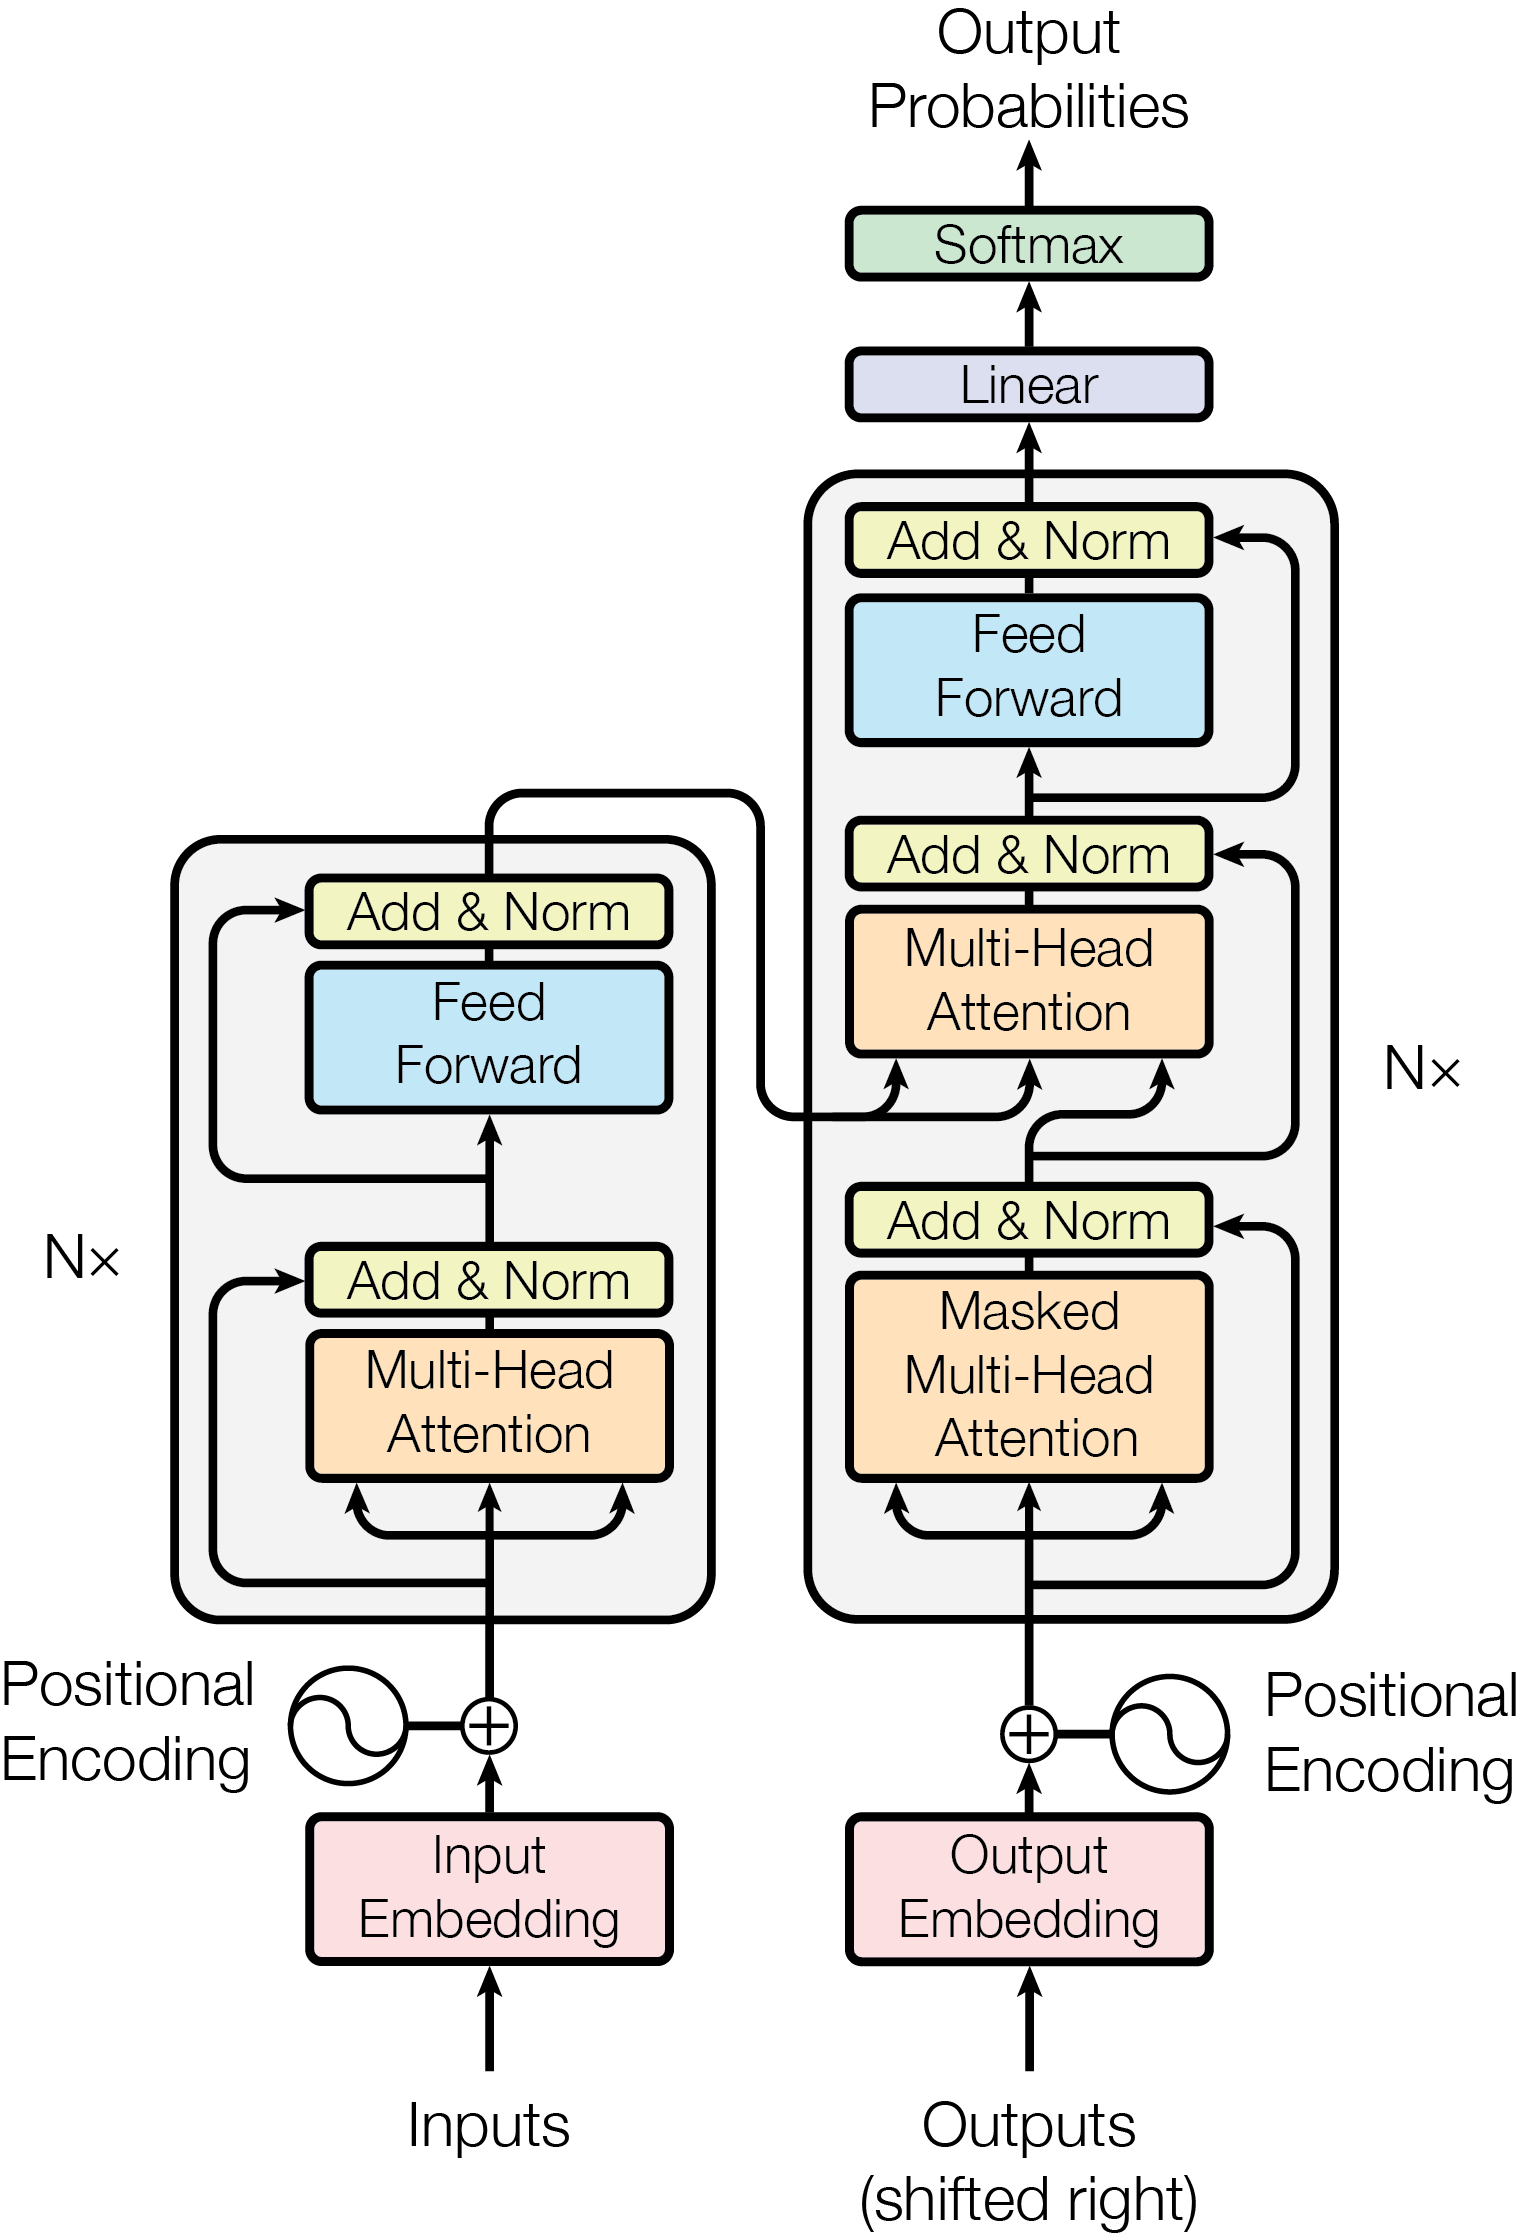
\includegraphics[width=0.6\linewidth]{figures/transformer.png}
    \caption{原始的Transformer模型架构\cite{Vaswani2017AttentionIA}，包含一个编码器和一个解码器。}
    \label{fig:trm}
\end{figure}

\paragraph{自注意力机制}
自注意力机制是Transformer的核心。它允许模型在处理一个序列时，为序列中的每个标记动态地计算其与序列中所有其他标记的关联权重。具体来说，对于每个输入标记，模型会生成三个向量：查询向量（Query, Q）、键向量（Key, K）和值向量（Value, V）。其核心计算过程为“缩放点积注意力”（Scaled Dot-Product Attention），其公式如下：
\begin{equation}
\text{Attention}(Q, K, V) = \text{softmax}\left(\frac{QK^T}{\sqrt{d_k}}\right)V.
\end{equation}
其中，$Q, K, V$ 分别代表由输入序列的查询、键、值向量堆叠而成的矩阵。$d_k$ 是键向量的维度。计算查询矩阵 $Q$ 和键矩阵转置 $K^T$ 的点积，得到原始的注意力得分。除以缩放因子 $\sqrt{d_k}$ 是为了防止点积结果过大，导致softmax函数进入梯度极小的区域，从而稳定训练过程。最后，归一化后的注意力权重会应用于值矩阵 $V$，得到加权的输出表示。

\paragraph{前馈网络}
Transformer的每个编码器和解码器层中，除了注意力子层外，还包含一个位置全连接的前馈网络（Position-wise Feed-Forward Network, FFN）。该网络通常由两个线性变换和一个非线性激活函数组成。对于注意力子层的输出向量 $x$，其计算过程可以表示为：
\begin{equation}
\text{FFN}(x) = \sigma(xW_1 + b_1) W_2 + b_2.
\end{equation}
其中，$W_1, b_1$ 和 $W_2, b_2$ 分别是第一个和第二个线性层的权重矩阵和偏置，$\sigma$表示非线性激活函数，常用GELU（Gaussian Error Linear Unit）\cite{Hendrycks2016GaussianEL}或ReLU\cite{Nair2010RectifiedLU}。$x \in \mathbb{R}^{d_{\text{model}}}$ 表示输入，第一个线性层通常将输入从 $d_{\text{model}}$ 维度扩展到 $d_{\text{ffn}}$（通常 $d_{\text{ffn}} = 4 \times d_{\text{model}}$），第二个线性层再将其映射回 $d_{\text{model}}$。前馈网络对每个词元（token）的向量表示进行独立的非线性变换，增加了模型的表达能力，并且占据了Transformer模型中大部分的参数量。

\paragraph{门控线性单元（GLU）及其变体}
门控线性单元（Gated Linear Unit, GLU）\cite{Shazeer2020GLUVI}是一种通过门控机制控制信息流的前馈网络变种，在如今为大多数开源大语言模型所采用，如LLaMA\cite{Touvron2023LLaMAOA}和Qwen\cite{Bai2023QwenTR}。它旨在增强模型的非线性表达能力。其核心思想是将输入向量通过两个不同的线性变换，并使用一个分支的输出作为“门”来调制另一个分支的输出。对于输入向量 $x$，基础GLU的计算过程可表示为：
\begin{equation}
\text{GLU}(x) = (xW_1 + b_1) \odot \sigma(xW_2 + b_2).
\end{equation}
其中，$W_1, W_2 \in \mathbb{R}^{d_{\text{model}} \times d_{\text{ffn}}}$ 为权重矩阵，$b_1, b_2$ 为偏置项，$\sigma$表示激活函数，$\odot$ 表示逐元素乘法。带激活函数的“门”分支可以起到抑制或放大信息的作用。GLU中的激活函数可以是ReLU（ReGLU）或GELU（GEGLU）等函数，例如GEGLU定义为：
\begin{equation}
\text{GEGLU}(x) = (xW_1 + b_1) \otimes \text{GELU}(xW_2 + b_2).
\end{equation}
在如今的开源大语言模型中，门控线性单元最常用的激活函数是$\text{Swish}$:
\begin{equation}
    \text{Swish}(x) =  x\cdot \text{sigmoid}(x) = x\cdot\frac{1}{1+e^{-x}}.
\end{equation}
门控线性单元结构通过门控机制实现了对特征的自适应筛选，增强了模型的表达能力。特别地，为了对齐普通前馈网络的参数量（ $d_{\text{ffn}} = 4 \times d_{\text{model}}$ ），门控线性单元的中间维度通常取$d_{\text{ffn}} = \frac{8}{3} \times d_{\text{model}}$。

\paragraph{位置编码}
由于自注意力机制本身不包含任何关于序列顺序的信息（即排列不变性），为了让模型能够利用序列的顺序，Transformer引入了位置编码（Positional Encoding）的概念。最早的位置编码是绝对位置编码。具体地，它用一个与输入词向量维度相同的向量，来标记词向量在序列中的绝对位置信息。这些位置编码向量被加到输入词向量上\cite{Vaswani2017AttentionIA}，从而将位置信息注入模型。如今的主流位置编码则是以相对位置编码为主，其中最具代表性的是旋转位置编码（Rotary Position Embedding, RoPE）\cite{Su2021RoFormerET}。旋转位置编码的核心思想是，不再将位置信息作为独立的向量加到词向量上，而是通过旋转的方式将位置信息融合到查询（Query）和键（Key）向量中。具体来说，它将一个 $d$ 维的向量 $\mathbf{x}$ 的维度两两分组，并将每一组 $(\boldsymbol{x}_{2i-1}, \boldsymbol{x}_{2i})$ 视为一个在复平面上的数。对于位于序列第 $m$ 个位置的向量，旋转位置编码会对每一组应用一个旋转矩阵，旋转角度与位置 $m$ 和维度索引 $i$ 相关。对向量 $\mathbf{q}_m$ (在位置 $m$ 的查询向量) 和 $\mathbf{k}_n$ (在位置 $n$ 的键向量) 应用旋转位置编码变换后，它们的点积 $(\mathbf{q}'_m)^T \mathbf{k}'_n$ 仅依赖于它们的原始内容向量 $\mathbf{q}, \mathbf{k}$ 和相对位置 $m-n$。
施加旋转位置编码的过程可以表示为对每个二维子空间的旋转。对于向量 $\mathbf{x}_m$ 的第 $2i-1$ 和 $2i$ 维，其变换如下：
\begin{equation}
\begin{pmatrix} x'_{m, 2i-1} \\ x'_{m, 2i} \end{pmatrix} = \begin{pmatrix} \cos(m\theta_i) & -\sin(m\theta_i) \\ \sin(m\theta_i) & \cos(m\theta_i) \end{pmatrix} \begin{pmatrix} x_{m, 2i-1} \\ x_{m, 2i} \end{pmatrix}
\end{equation}
其中，$\theta_i = 10000^{-2i/d}$ 是一个预设的、随维度增加而减小的旋转基频率。通过这种方式，注意力得分的计算天然地编码了相对位置信息，同时该方法具有良好的外推性，能够更好地处理比训练时更长的序列。旋转位置编码已成为众多现代大规模语言模型（如LLaMA系列）的标准配置。


\section{混合专家模型简介}

混合专家模型（Mixture-of-Experts, MoE）是一种神经网络架构，它通过条件计算来激活模型参数的一个稀疏子集，而非像传统稠密模型（dense model）那样在每次前向传播中激活所有参数。这一思想最早可以追溯到Jacobs等人的研究 \cite{Jacobs1991AdaptiveMO}，并在近年来被成功应用于大规模语言模型中，用以解决模型扩展性与计算效率之间的矛盾。在大语言模型中，混合专家模型主要用于替换前馈网络层。一个典型的混合专家模型层主要由两个核心组件构成：多个专家网络（较小规模的前馈神经网络层）和一个路由器（或称为门控网络, Gating Network）。图\ref{fig:densevsmoe}展示了混合专家模型和稠密模型的区别。

\begin{figure}[h]
    \centering
    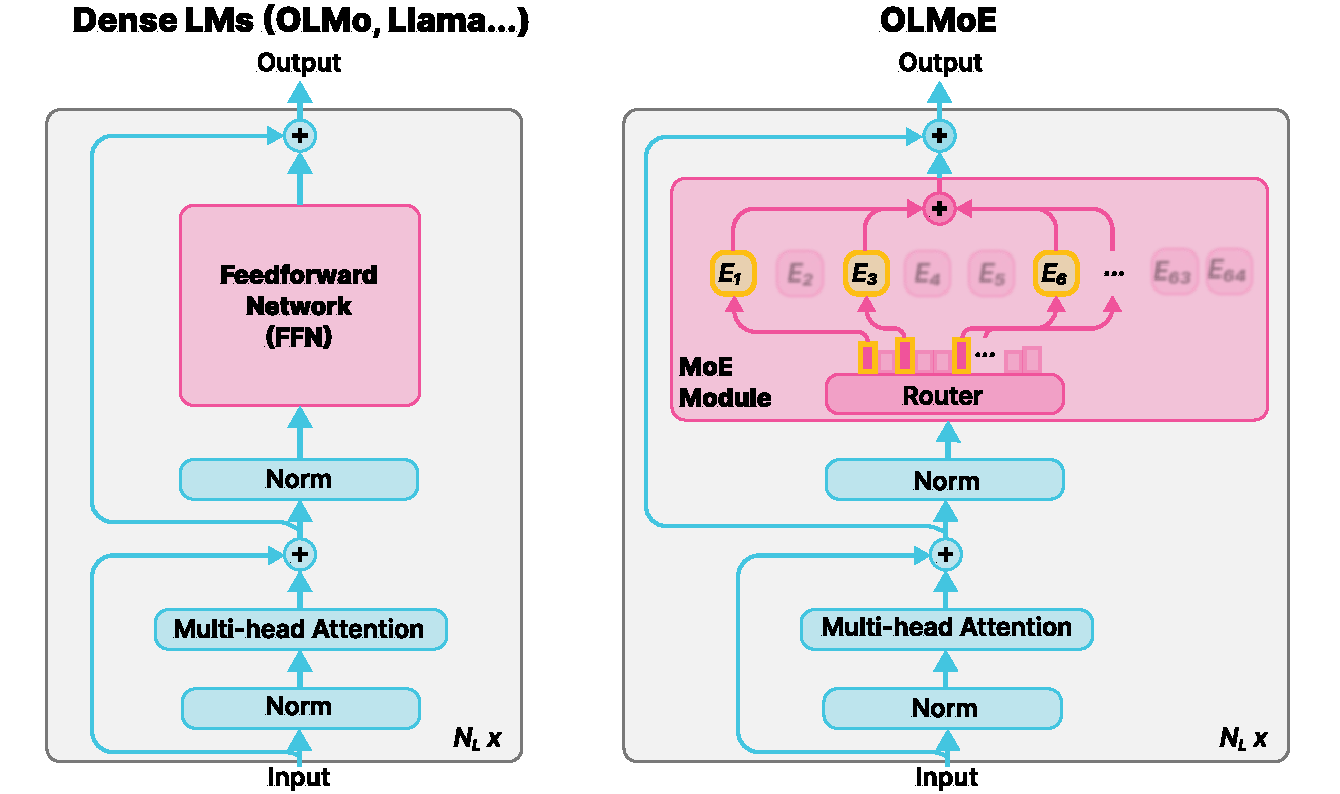
\includegraphics[width=0.9\linewidth]{figures/olmoe.pdf}
    \caption{混合专家模型（以OLMoE\cite{Muennighoff2024OLMoEOM}为例）和稠密模型的区别}
    \label{fig:densevsmoe}
\end{figure}

\paragraph{条件计算}

条件计算（Conditional Computation）是现代混合专家模型的核心思想。传统的神经网络在处理所有输入时，都使用完全相同的参数集合。与之相反，混合专家模型包含多个“专家”子网络，并为每个输入动态地选择一小部分专家来处理。这意味着，尽管模型的总参数量可以非常庞大（例如，由成百上千个专家组成），但对于单个输入词元（token）的处理，其计算路径是稀疏的，实际参与计算的参数量和计算量都远小于总参数量。这种方式打破了模型总参数量与计算量之间的固定耦合关系，使得在有限的计算预算下构建参数规模极其庞大的模型成为可能 \cite{Shazeer2017OutrageouslyLN}。

\paragraph{专家}
专家（Experts）是混合专家模型中执行具体计算的子网络。在基于Transformer的语言模型中，专家通常就是前馈网络（FFN）。假设一个MoE层有 $N$ 个专家，对于输入向量 $x$，第 $i$ 个专家 $E_i$ 的计算过程与其替代的密集FFN层一致：
\begin{equation}
E_i(x) = \text{GELU}(xW_{1,i} + b_{1,i}) W_{2,i} + b_{2,i}
\end{equation}
每个专家 $E_i$ 都拥有自己独立的参数 $\{W_{1,i}, b_{1,i}, W_{2,i}, b_{2,i}\}$。在训练过程中，通常认为，不同的专家会趋向学习并“专精于”处理不同类型的数据模式\cite{Xue2024OpenMoEAE}。

\paragraph{路由器 (Router)}
路由器的作用是为每个输入的词元 $x$ 决定应该由哪些专家来处理。它通过一个可学习的线性变换 $W_g$ 计算每个专家的得分（logits）：
\begin{equation}
h(x) = x W_g
\end{equation}
其中 $h(x) \in \mathbb{R}^{N}$ 是一个包含 $N$ 个专家得分的向量。在稀疏的Top-k路由策略中，路由器会从 $h(x)$ 中选择得分最高的 $k$ 个值。设这 $k$ 个专家的索引集合为 $\mathcal{T}$。然后，仅对这 $k$ 个得分应用Softmax函数（或其他激活函数）来计算它们的权重（门控值）：
\begin{equation}
G(x)_i = \begin{cases} \frac{e^{h(x)_i}}{\sum_{j \in \mathcal{T}} e^{h(x)_j}} & \text{if } i \in \mathcal{T} \\ 0 & \text{if } i \notin \mathcal{T} \end{cases}
\end{equation}
最终，混合专家模型层的输出 $y$ 是被选中的 $k$ 个专家输出的加权和：
\begin{equation}
y = \sum_{i \in \mathcal{T}} G(x)_i \cdot E_i(x)
\end{equation}
这个公式清晰地体现了条件计算的本质：只有索引在 $\mathcal{T}$ 中的少数专家被激活并参与计算，而它们的贡献由路由器动态计算的权重 $G(x)_i$ 决定。

\paragraph{专家并行}
专家并行（Expert Parallelism）（图\ref{fig:ep}）是专门为混合专家模型设计的一种模型并行（Model Parallelism）策略，旨在解决其巨大的内存占用问题。在标准的数据并行中，每个计算设备（如GPU）都保存一份完整的模型副本，这对于拥有数万亿参数的混合专家模型来说是不可行的。专家并行策略则将混合专家模型层中的 $N$ 个专家划分到 $M$ 个设备上，每个设备仅负责存储和计算其中的 $N/M$ 个专家。模型中的共享部分（如自注意力层和路由器）则在所有设备上进行复制。在训练的前向传播过程中，每个设备上的路由器为本地的词元批次做出路由决策。随后，通过一个高效的All-to-All通信操作，将需要由特定专家处理的词元发送到持有该专家的相应设备上。在各自的设备上完成专家计算后，再通过另一次All-to-All通信将计算结果发送回原始设备进行加权求和。这种方式虽然引入了额外的通信开销，但它极大地降低了单个设备的内存需求，使得训练远超单卡内存容量的巨型混合专家模型成为可能。

\begin{figure}[h]
    \centering
    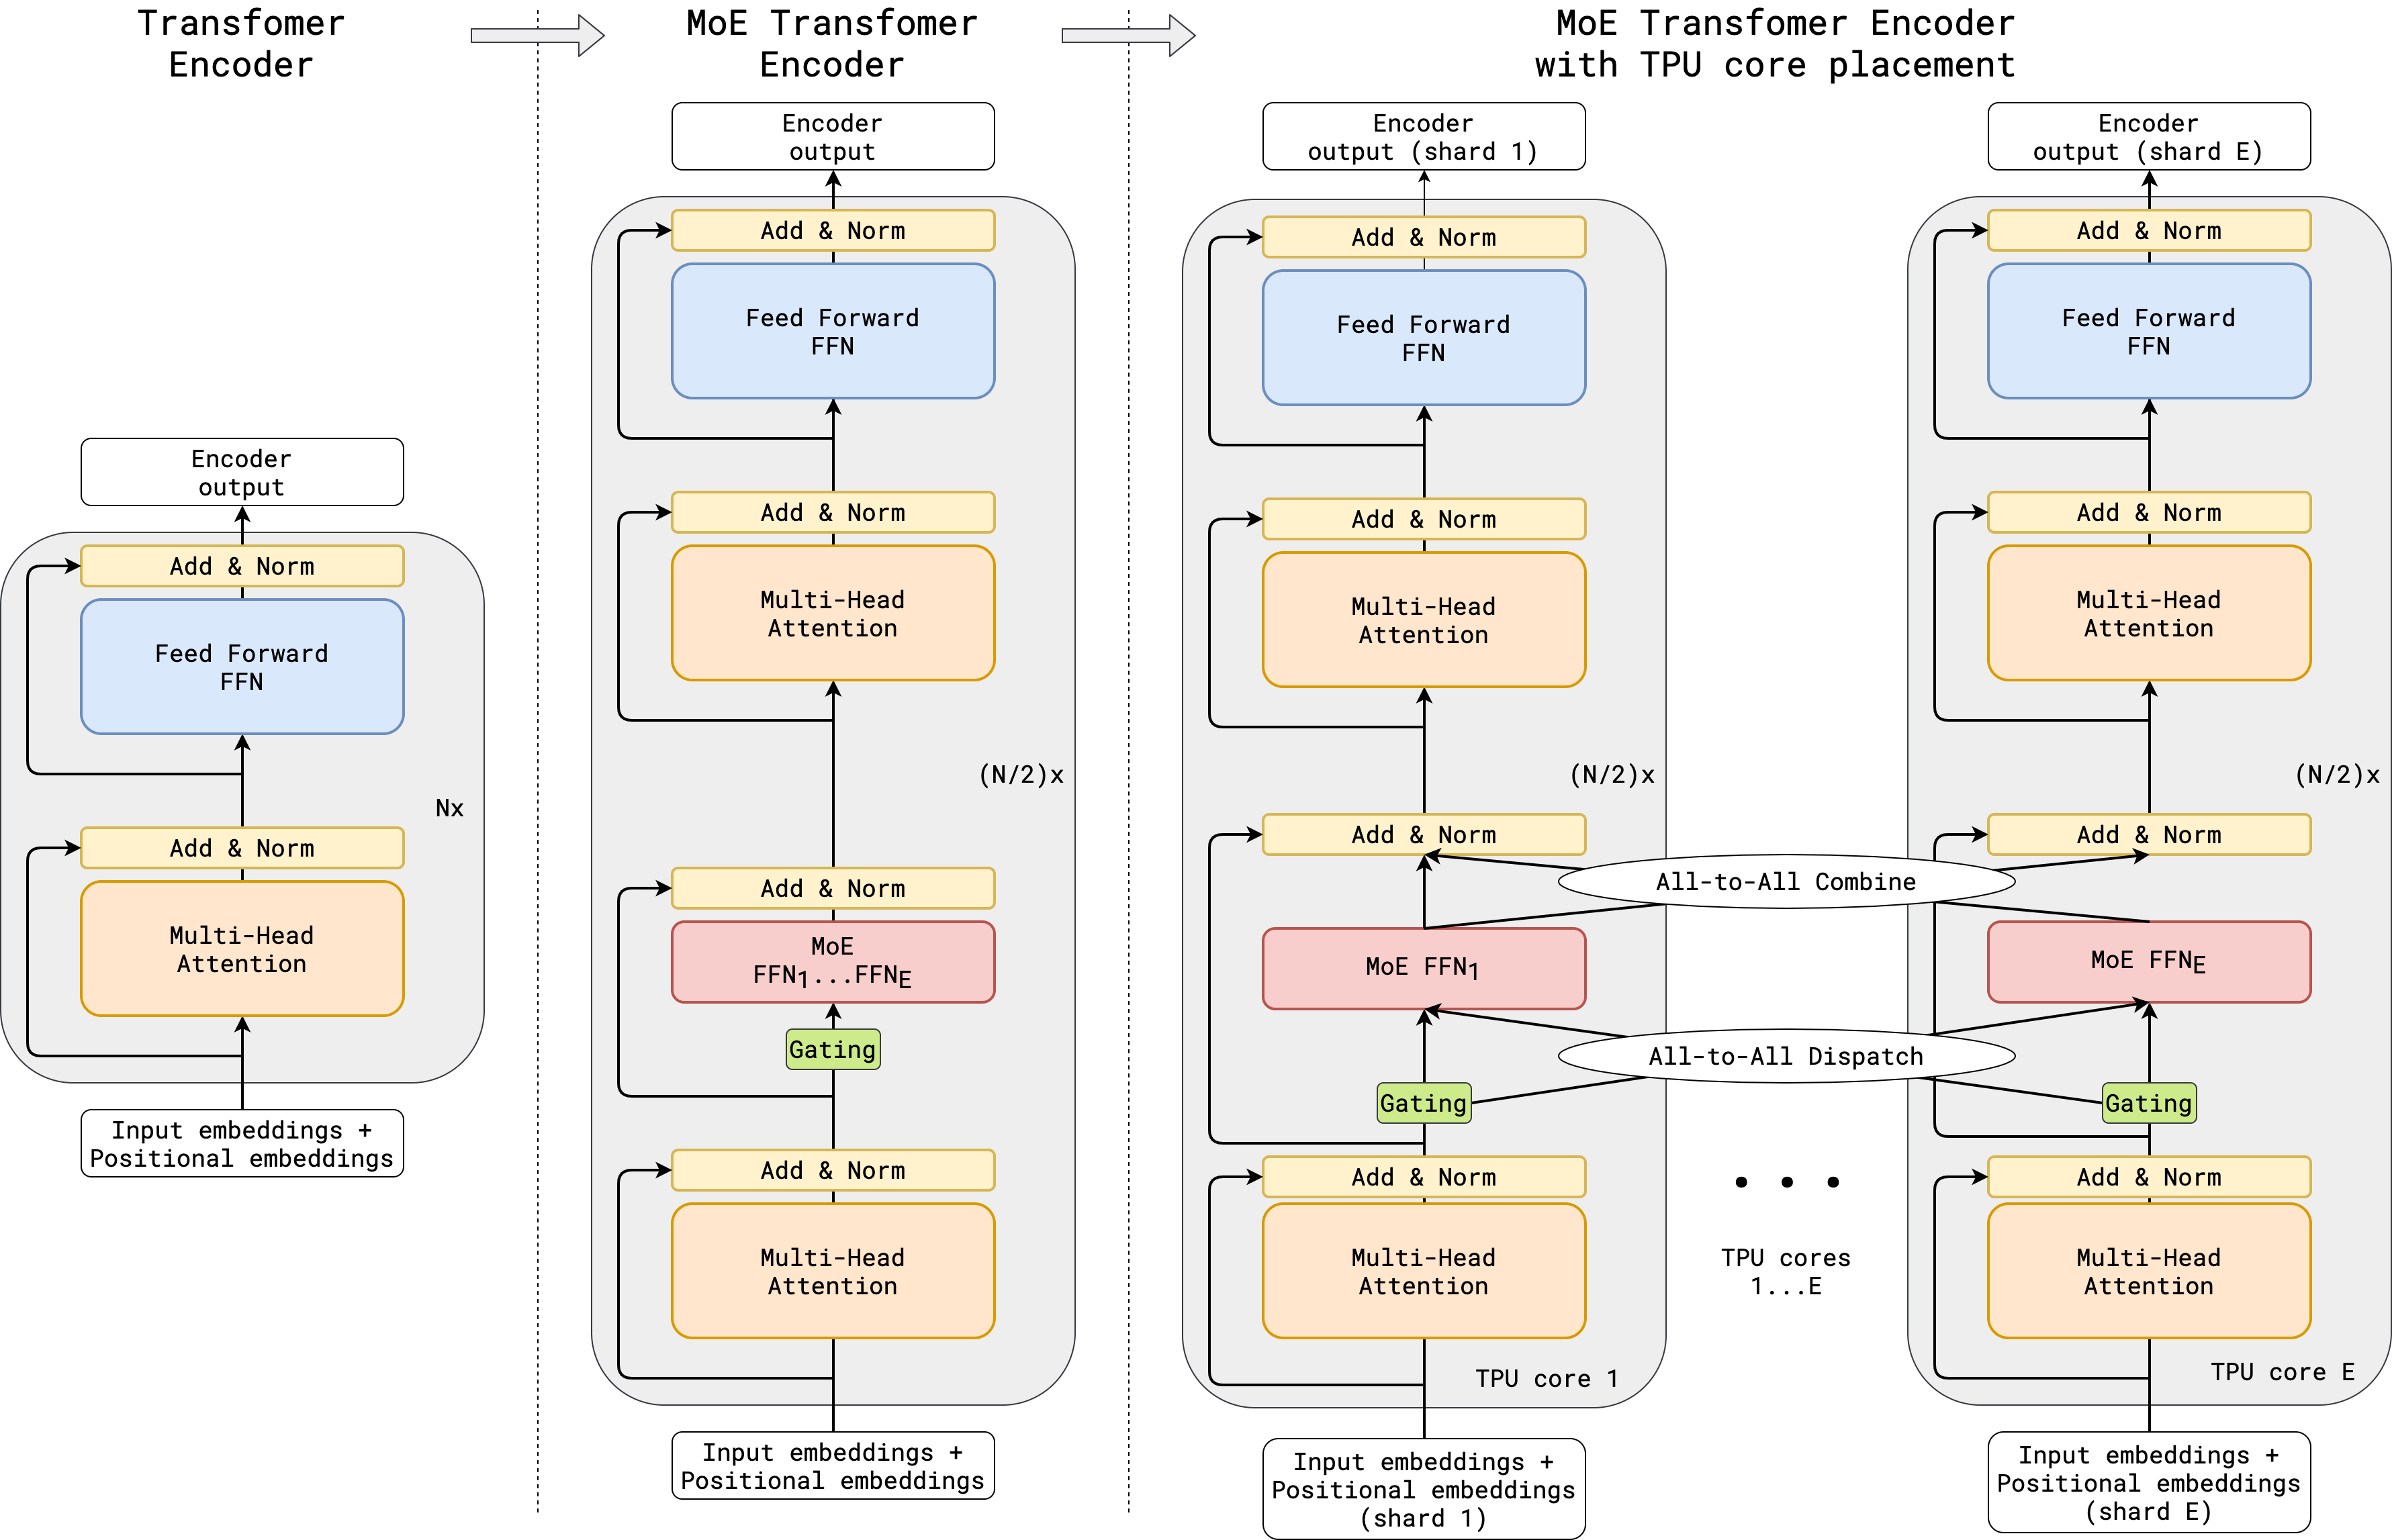
\includegraphics[width=1.0\linewidth]{figures/moe.png}
    \caption{GShard\cite{Lepikhin2020GShardSG}中的专家并行（以编码器部分为例，解码器亦类似）}
    \label{fig:ep}
\end{figure}

\section{预训练大语言模型}

预训练大语言模型（Pre-trained Large Language Models, LLMs）是指在一系列大规模、多样化的无标注文本语料上进行预训练，然后在各种下游任务上进行微调（fine-tuning）或在零/少样本（zero/few-shot）场景下使用的模型。这一范式已成为现代自然语言处理的基石，其成功的核心在于通过大规模数据和模型参数，让模型学习到通用的语言表征和世界知识。

\paragraph{自监督预训练}
LLMs 的核心技术是自监督学习（Self-supervised Learning）。与需要大量人工标注数据的监督学习不同，自监督学习从无标注数据本身创造学习信号。在NLP领域，主要有两种主流的预训练目标：
\begin{itemize}
    \item \textbf{自回归语言建模 (Autoregressive Language Modeling)}: 这是GPT系列模型 \cite{Radford2018ImprovingLU} 采用的核心目标。模型被训练来预测序列中的下一个词元（token），其目标函数是最大化给定上文条件下，下一个真实词的条件概率。对于一个词元序列 $X = (x_1, x_2, \dots, x_T)$，其似然函数为：
    \begin{equation}
    L(X) = \sum_{t=1}^{T} \log P(x_t | x_{<t}; \Theta)
    \end{equation}
    其中 $\Theta$ 代表模型参数。这种从左到右的单向建模方式天然适用于文本生成任务。

    \item \textbf{掩码语言建模 (Masked Language Modeling, MLM)}: 这是BERT \cite{Devlin2019BERTPO} 及其变体所开创的目标。训练时，输入序列中会随机遮盖（mask）掉一部分词元，模型的任务是根据其左右双向的上下文来预测这些被遮盖的词元。这种方式使得模型能够学习到深度的双向语境表征，因此在自然语言理解（NLU）任务上表现尤为出色。
\end{itemize}
通过在数千亿甚至上万亿词元的语料上进行预训练，模型能够内化丰富的语法结构、语义关系、语用知识乃至海量的世界知识。

\paragraph{从微调到上下文学习的范式演进}
早期的预训练模型（如BERT）主要遵循“预训练-微调”范式。模型首先完成通用知识的学习，然后针对特定的下游任务（如情感分析、命名实体识别等），使用该任务的标注数据对模型的全部或部分参数进行微调。然而，随着模型规模的急剧增大（如GPT-3达到1750亿参数），一种新的、更灵活的交互范式——\textbf{上下文学习}（In-Context Learning, ICL）——应运而生\cite{Brown2020LanguageMA}。上下文学习指的是大语言模型能够在不更新任何模型权重的情况下，仅通过在输入提示（prompt）中提供任务描述和/或少数示例，就能理解并执行新任务。这种能力根据示例的数量分为：
\begin{itemize}
    \item \textbf{零样本学习 (Zero-shot Learning)}: 只提供任务的自然语言描述，不提供任何示例。
    \item \textbf{少样本学习 (Few-shot Learning)}: 提供任务描述和少量（通常为1到几十个）输入-输出示例。
\end{itemize}
上下文学习的出现极大地降低了模型适应新任务的门槛，使得与单一模型进行对话式交互来解决多种问题成为可能，这也是当前大语言模型应用的主流形式。

\paragraph{缩放法则}
研究表明，大语言模型的性能与其规模之间存在着紧密且可预测的关系，这被称为\textbf{缩放法则} (Scaling Laws)\cite{Kaplan2020ScalingLF}。该法则指出，模型的性能（通常以测试集上的损失函数值来衡量）是模型所用计算量（C）、训练数据量（D）和参数量（N）的幂律函数（如图\ref{fig:scaling_law}所示）。这意味着，只要协同地、按比例地增加这三个要素，模型的性能就会持续提升。缩放法则为投入巨量资源构建更大模型提供了理论指导，也正是驱动模型走向万亿参数规模的根本动力。

\begin{figure}[h]
    \centering
    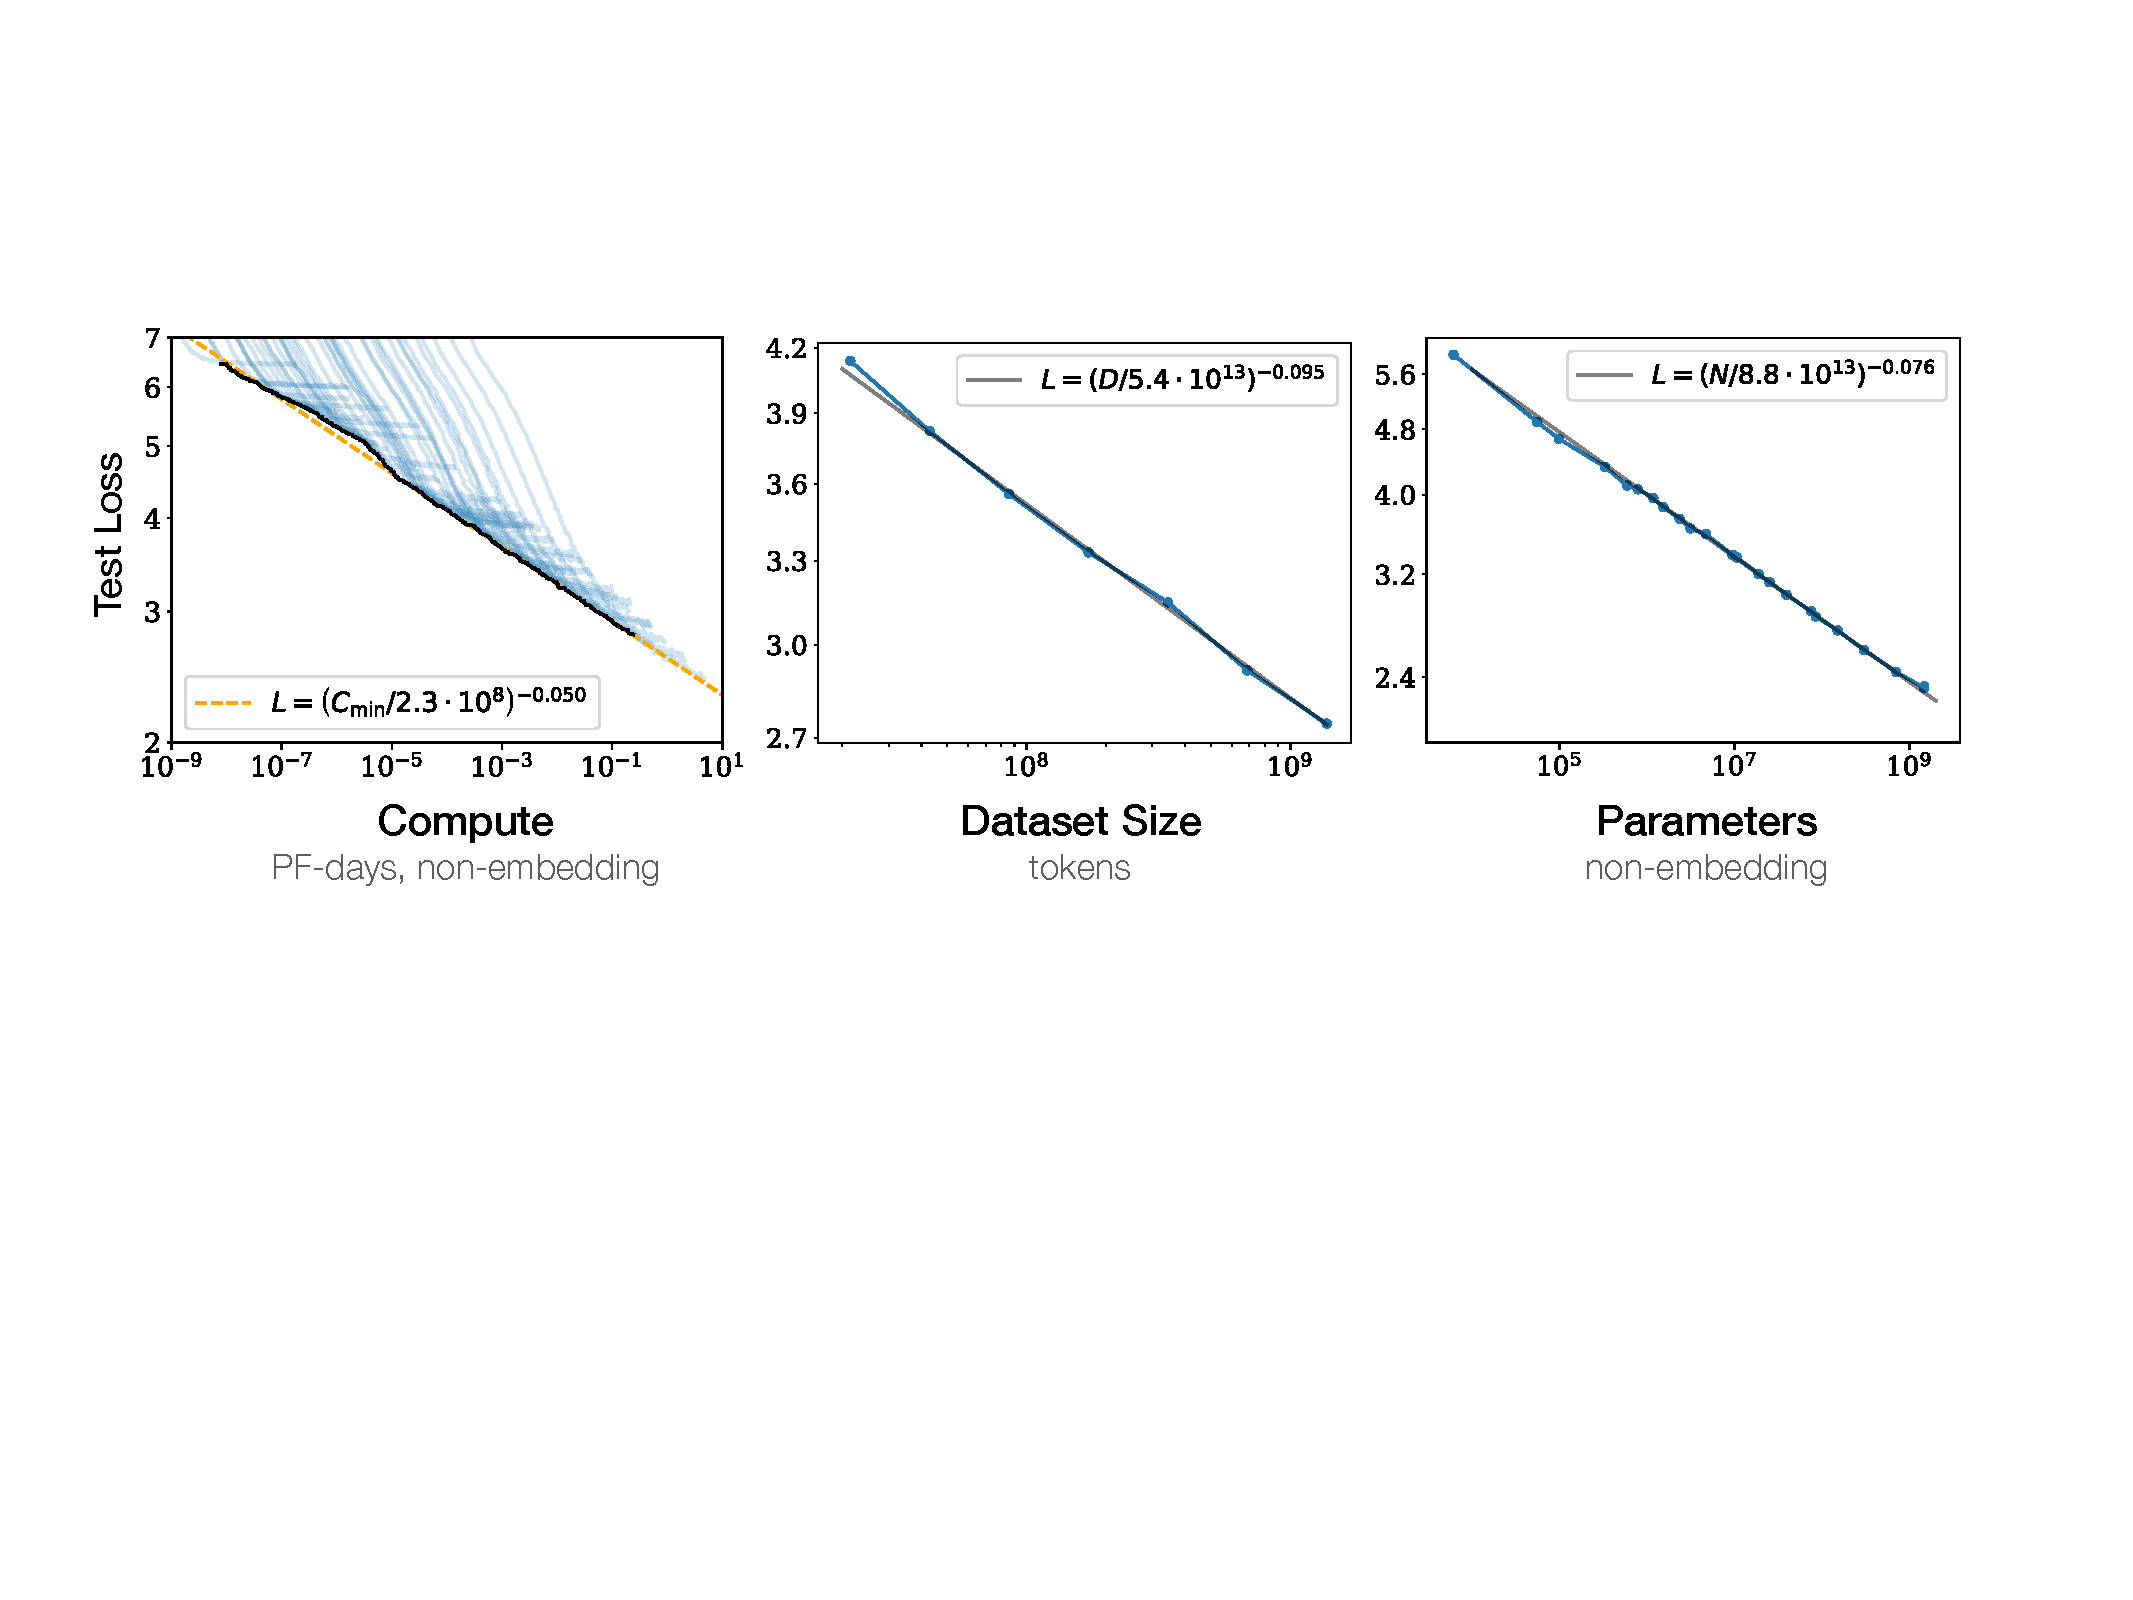
\includegraphics[width=1.0\linewidth]{figures/SimplePowerLaws.pdf}
    \caption{缩放法则指出，模型的性能（测试集上的损失函数值）是模型所用计算量、训练数据量和参数量的幂律函数\cite{Kaplan2020ScalingLF}。}
    \label{fig:scaling_law}
\end{figure}


\paragraph{涌现能力} 有趣的是，当模型规模跨越某个临界点后，它们会表现出许多在小规模模型上未曾出现的\textbf{涌现能力} (Emergent Abilities) \cite{Wei2022EmergentAO}（图\ref{fig:emergent}）。这些能力并非随着模型规模的增大而平滑地提升，而是在某个规模上“突然”出现。典型的例子包括多步算术推理、遵循复杂指令的能力，以及“思维链”（Chain-of-Thought, CoT）推理能力\cite{Wei2022ChainOT}——即通过引导模型分步思考来解决复杂问题。这些高级认知能力的涌现，进一步印证了扩大模型规模与计算量的重要性。
\begin{figure}[h]
    \centering
    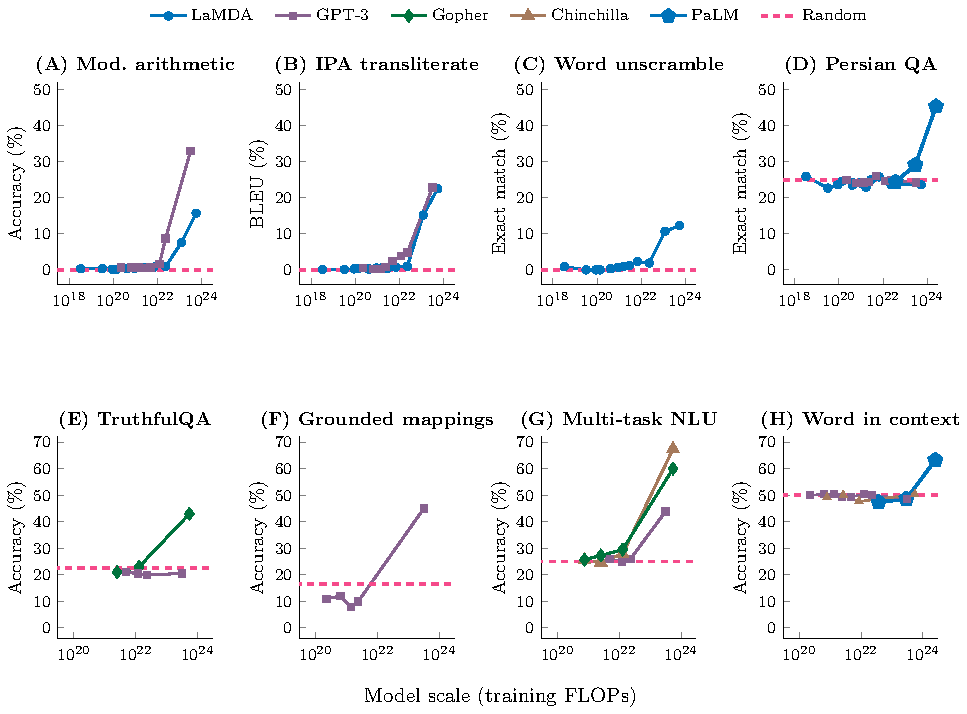
\includegraphics[width=1.0\linewidth]{figures/emergent.pdf}
    \caption{模型规模在跨越某个临界点后，展现出能力的突然提升\cite{Wei2022EmergentAO}。}
    \label{fig:emergent}
\end{figure}

\paragraph{训练效率与模型FLOPS利用率 (MFU)}
在实践中，要有效地实现缩放法则所预测的性能增益，仅仅提供理论上的计算量（FLOPs）是不够的，还必须确保硬件的计算潜力被充分利用。为此，业界提出了\textbf{模型FLOPS利用率}（Model FLOPs Utilization, MFU）这一关键工程指标 \cite{Chowdhery2022PaLMSL}。模型FLOPS利用率衡量的是在模型训练过程中，硬件（如GPU）实际达到的持续浮点运算速度与硬件理论峰值浮点运算速度的比率。一个高的模型FLOPS利用率意味着训练代码和系统架构能够高效地让硬件执行其最擅长的矩阵运算。然而，由于数据加载、GPU间的通信开销、非矩阵运算操作以及内存带宽限制等瓶颈，实现高模型FLOPS利用率是一项巨大的系统工程挑战。因此，优化训练效率、最大化模型FLOPS利用率，是降低训练成本、加速模型迭代、并最终在给定计算预算内触及缩放法则性能上限的核心环节。表\ref{table:training-efficiency}列出了一些模型的模型FLOPS利用率（MFU）。

\begin{table}[h!]
    \setlength{\tabcolsep}{6pt}
    \centering
    \small
    \begin{tabular}{lc cc}
    \toprule
     模型 & \makecell[c]{参数量(十亿)}  &  加速器芯片 & \makecell[c]{模型FLOPS利用率} \\
    \midrule
    GPT-3 & 175B &  V100 & 21.3\%  \\
    Gopher & 280B &  4096 TPU v3 & 32.5\%  \\
    Megatron-Turing NLG & 530B & 2240 A100 & 30.2\%  \\
    PaLM & 540B &  6144 TPU v4 & 46.2\% \\
    \bottomrule
    \end{tabular}
    \caption{一些模型的模型FLOPS利用率（MFU）\cite{Chowdhery2022PaLMSL}}
    \label{table:training-efficiency}
\end{table}

\paragraph{训练稳定性与损失尖峰的挑战}
在数百亿乃至万亿参数的规模下，预训练不仅是一项科学探索，更是一项对工程能力的巨大考验，其中\textbf{训练的稳定性}至关重要。在大规模训练中最常见也最棘手的失败模式是\textbf{损失尖峰 (loss spike)}：即训练损失（loss）突然发生灾难性的飙升，其值可能发散至无穷大 (`Inf`) 或变为无效数字 (`NaN`)。单次此类事件就足以破坏模型已学习到的权重，迫使研究人员中断进程，并回退到很早之前的稳定检查点 (checkpoint)，从而浪费数周甚至数月的宝贵计算资源。因此，理解并缓解这一不稳定性的根源，是LLM工程中的核心关切。

损失尖峰的根本原因是数值不稳定性，其来源多种多样：
\begin{itemize}
    \item \textbf{梯度爆炸 (Gradient Explosion)}\cite{Pascanu2012OnTD}: 这是最直接的原因。由于Transformer架构深度堆叠的链式特性，反向传播有时会导致梯度呈指数级增长。这会产生极大的权重更新，使得模型参数“越过”损失地貌 (loss landscape) 中的最优点，被抛入一个损失值高得多的区域，并可能再也无法从中恢复。

    \item \textbf{浮点数精度问题}: 为了加速训练并减少显存占用，LLMs通常采用低精度数值格式，其有限的动态范围使其极易出现上溢 (overflow，数值过大无法表示) 和下溢 (underflow，数值过小变为零) 的问题。为此，往往需要对不同模块设置合适的数值精度，并采取适当的量化方法，来保证训练的稳定性。

    \item \textbf{异常数据}: 庞大且通常混杂的预训练语料库中，可能包含格式错误或异常的数据点。这些数据点会产生异常大的损失值和梯度，从而成为触发不稳定的导火索。
\end{itemize}

为了应对这些问题，研究者们需要协同采用若干技术，如梯度裁剪（gradient clipping），权重衰减（weight decay）和归一化（Normalization）来稳定训练\cite{Rybakov2024MethodsOI,Wortsman2023SmallscalePF}。
在混合专家 (MoE) 模型中，这些挑战可能会变得更加复杂，因为其路由机制引入了额外的动态且可能不稳定的行为层（例如路由器的表示坍缩）。

% 这里补一张涌现能力的图片，然后后面再补一个概念/或者在moe那里补一个/或者前面补张图/最后补一下MFU的概念介绍？

% 后面moe可以提一下并行策略之类的，还有负载均衡;后面介绍的工作也可以讲讲偏向mlsys的？如果方便的话，写起来麻烦就算了
% 后面可以加一章介绍现代开源moe模型的典型结构

        \chapter{混合专家模型架构与训练}
\label{chap:mox_training}

混合专家模型（Mixture-of-Experts, MoE）的引入是近年来大规模语言模型（Large Language Models, LLMs）发展中的一项关键创新。通过将传统Transformer架构中密集计算的前馈网络（Feed-Forward Network, FFN）层替换为由多个并行且独立的“专家”网络和一个动态“路由器”（Router）组成的\textbf{稀疏激活模块}，混合专家模型成功地解耦了模型的总参数量与单样本前向传播的计算量（FLOPs）。这一设计使得模型能够在保持计算成本相对恒定的前提下，将参数规模扩展至前所未有的万亿级别，从而显著提升模型容量与性能。本章将详细梳理经典的稀疏混合专家模型架构，深入剖析其核心技术——路由算法的多种实现及其演进，探讨专家网络的设计考量，并系统阐述混合专家模型模型在训练过程中面临的关键挑战及其主流解决策略。

\section{经典的稀疏混合专家模型架构}

经典的稀疏混合专家模型架构最早由 Shazeer等人\cite{Shazeer2017OutrageouslyLN}引入到深度学习模型中，并由 Lepikhin 等人在 GShard\cite{Lepikhin2020GShardSG}中成功应用于大规模Transformer模型。其核心思想是，在Transformer的每个块（Block）中，用一个混合专家模型层来替换原有的前馈网络层。一个混合专家模型层主要由两个核心组件构成：
\begin{itemize}
    \item \textbf{专家网络 (Experts)}: 这通常是一组在结构上相同但在参数上相互独立的网络。在Transformer架构中，每个专家就是一个标准的前馈网络模块，包含两个线性层和一个非线性激活函数（如GELU或SwiGLU）。专家网络的数量 $N$ 可以从几十个扩展到数千个。
    \item \textbf{门控网络/路由器 (Gating Network/Router)}: 这是一个小型神经网络，通常是一个简单的线性层。其核心功能是实现\textbf{条件计算}（Conditional Computation）：为序列中的每一个输入词元（Token）动态地、稀疏地选择一个或少数几个（$k$个）最合适的专家进行处理。
\end{itemize}
如图\ref{fig:moe_module}所示，在一次前向传播中，对于输入序列中的词元 $\mathbf{x}$，路由器会计算出一个该词元与所有 $N$ 个专家之间的亲和度得分（logits），记为 $h(\mathbf{x})$。基于此得分，模型选择得分最高的 $k$ 个专家，其索引集合记为 $\text{TopK}(h(\mathbf{x}))$。

随后，词元 $\mathbf{x}$ 的表征被送入这些被选中的专家网络进行计算，得到各自的输出 $E_i(\mathbf{x})$。与此同时，对应 $k$ 个专家的得分会经过Softmax函数计算，生成归一化的门控权重（Gating Weights）$G(\mathbf{x})_i$。最终，MoE层的总输出 $\mathbf{y}$ 是这些专家输出的加权和：

\begin{equation}
    \mathbf{y} = \sum_{i \in \text{TopK}(h(\mathbf{x}))} G(\mathbf{x})_i \cdot E_i(\mathbf{x}).
\end{equation}
通过这种方式，虽然模型总参数量因 $N$ 个专家的存在而大幅增加，但每个词元的计算路径只激活了其中 $k/N$ 的参数，从而在不显著增加计算量的情况下实现了模型容量的巨大扩展。

\begin{figure}[h]
    \centering
    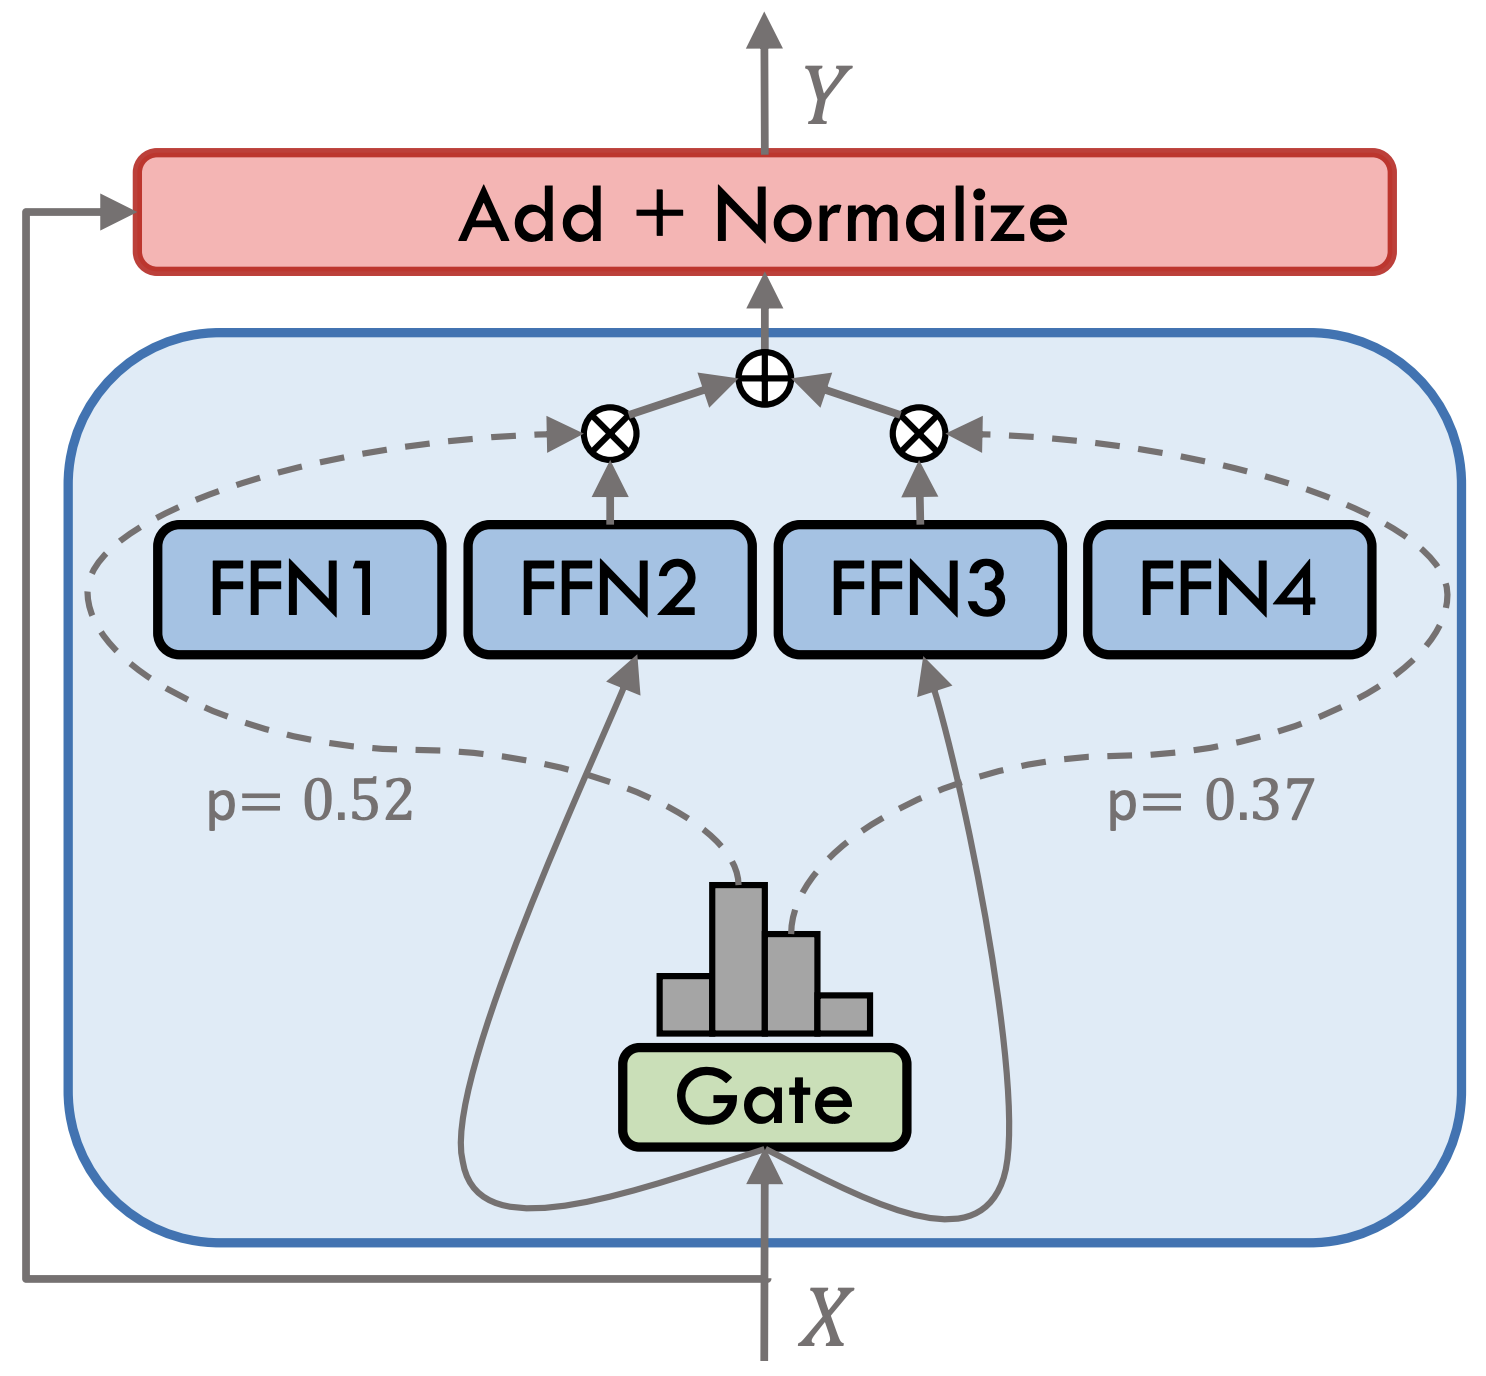
\includegraphics[width=0.6\linewidth]{figures/moe_module.jpg}
    \caption{混合专家模型层}
    \label{fig:moe_module}
\end{figure}

\section{经典Top-k路由算法}
\label{sec:classic_top-k}
路由算法是混合专家模型的心脏，其设计直接决定了模型的性能、训练稳定性以及计算效率。理想的路由算法应具备内容感知、负载均衡和计算高效等特性。目前最主流且被广泛应用的路由算法是由 Shazeer 等人\cite{Shazeer2017OutrageouslyLN}提出的基于\textbf{Top-k门控}的稀疏门控机制。对于输入词元 $\mathbf{x}$，路由器的计算过程如下：
\begin{enumerate}
    \item \textbf{（前向）计算路由Logits}: 路由器（一个线性层 $\mathbf{W}_g$）将词元 $\mathbf{x}$ 映射到维度等于专家数量 $N$ 的向量，得到路由Logits：$h(\mathbf{x}) = \mathbf{W}_g \mathbf{x}$。
    % \item \textbf{添加噪声 (可选)}: 为了在训练中促进路由决策的探索性并改善负载均衡，通常会向Logits中添加标准高斯噪声：$h(\mathbf{x})_{\text{noisy}} = h(\mathbf{x}) + \mathcal{N}(0, 1/N^2)$。
    \item \textbf{（前向）选择Top-k专家}: 从 $h(\mathbf{x})_{\text{noisy}}$ 中选取值最大的 $k$ 个维度，其对应的索引即为被选中的 $k$ 个专家的索引。具体地，在 Switch Transformer\cite{Fedus2021SwitchTS}中，$k$设置为了1，实现了极高的稀疏度（$N$最大为2048）；gpt-oss\cite{openai2025gptoss}选择了$k = 4$以及$N = 32$（20B模型）或$128$（120B模型），通过一个适中的稀疏度和较粗粒度的专家来平衡模型表现与推理效率；国内近期的大模型DeepSeek-V3\cite{DeepSeekAI2024DeepSeekV3TR}、Kimi K2\cite{Bai2025KimiKO}则分别选择了$k = 8,\ N = 256$与$k=8, N=384$，用类似gpt-oss的稀疏度但是更细粒度的专家（同等$k/N$下更大的$k$）来换取性能提升。
    \item \textbf{（前向）计算门控权重}: 对选出的 $k$ 个Logits应用Softmax函数或Sigmoid函数，生成归一化的门控权重（Gating Weights）$G(\mathbf{x})$。最初的混合专家模型以Softmax函数为主流\cite{Shazeer2017OutrageouslyLN,Lepikhin2020GShardSG,Fedus2021SwitchTS}，Sigmoid函数虽有尝试\cite{Lewis2021BASELS,Dai2022StableMoESR}，但未被广泛采用。不过，值得一提的事，近来国内开源的大模型有若干采用了Sigmoid函数作为路由器的激活函数\cite{DeepSeekAI2024DeepSeekV3TR,Bai2025KimiKO,Zeng2025GLM45AR}。
    \item \textbf{（反向）梯度直通估计 (Straight-Through Estimator)}：
    由于 \text{Top-k} 选择操作是离散且不可导的，标准的反向传播会在此处中断。为了训练路由器，模型采用了梯度直通估计（STE）\cite{Rosenblatt1958ThePA,Bengio2013EstimatingOP,Jang2016CategoricalRW,Liu2023BridgingDA}的技巧。其核心思想是，在反向传播时，我们为这个离散步骤手动定义一个“伪梯度”。我们首先考虑最终输出 $y = \sum_{i \in I} G_i(x) \cdot E_i(x)$，其中 $I$ 是被选中的 \text{Top-k} 专家索引集。梯度直通估计认为，损失 $L$ 对门控权重 $G_i$ 的梯度，只对那些被选中的专家（$i \in I$）有意义，其值与对应专家的输出 $E_i(x)$ 与输出的梯度$\frac{\partial L}{\partial y}$有关。利用多元链式法则，损失 $L$ 对标量门控权重 $G_i$ 的梯度（一个标量） ，是损失对输出向量 $y$ 的梯度（向量）与该专家输出 $E_i(x)$ （向量）的内积，亦即：
    \begin{equation}
        \frac{\partial L}{\partial G_i} = 
    \begin{cases}
        \nabla_y L \cdot E_i(x) & \quad \text{if } i \in I \\
        0 & \quad \text{if } i \notin I
    \end{cases}
    \end{equation}
    
    梯度直通估计的作用就是将这个计算出的梯度 $\frac{\partial L}{\partial G_i}$ 作为有效梯度，继续通过 Softmax 函数回传到路由器对应的 logit $h_i(x)$ 上。这样，尽管 \text{Top-k} 选择本身不可导，但路由器的参数 $W_g$ 依然能够接收到有效的学习信号并进行更新。
    
\end{enumerate}


% unfinished
\section{Top-k 路由的变体与优化}
尽管标准Top-k机制非常成功，但其局部贪心的性质可能导致次优的全局分配和负载不均衡。因此，工业界与学术界探索了多种变体以求改进。

\subsection{带随机性的Top-k路由} 
\paragraph{随机丢弃的Top-2路由} GShard\cite{Lepikhin2020GShardSG}出于负载均衡和训练推理效率的考虑，在\text{Top-2}路由中引入了依照第二个专家的概率分数（亦即对输出的权重）随机丢弃该专家的策略，丢弃的概率即$1 - G_i$。

\paragraph{带噪声的Top-k路由} 
Shazeer等人在其2017年提出的开创性工作\cite{Shazeer2017OutrageouslyLN}中引入了噪声机制，通过增加路由过程的随机性来促进负载均衡。其核心思想是在计算出的路由Logits送入Top-k选择逻辑之前，为其添加一个可学习的、与输入相关的噪声： 
\begin{equation}
h_{\text{noisy}}(x)_i = (x W_g)_i + \text{StandardNormal}() \cdot \text{Softplus}((x W{\text{noise}})_i)
\end{equation}
其中，$W_{\text{noise}}$ 是一个与路由权重矩阵 $W_g$ 相互独立的、可训练的权重矩阵，用于生成噪声的缩放因子。$\text{Softplus}$ 函数确保该因子始终为正。

值得注意的是，在如今的大语言模型中，这种随机噪声路由已经很少被采用。一方面，随机路由可能带来训练的不稳定性，增加训练噪声，降低训练效率，另一方面，随机路由也给推理部署时的表现带来了不确定性。

\subsection{全局优化的路由}
尽管经典的 \text{Top-k} 路由机制通过引入辅助损失函数能在一定程度上缓解负载不均衡问题，但这种基于启发式规则的局部优化方法仍然是影响混合专家模型性能与训练稳定性的普遍挑战。为了从根本上解决这一问题，研究者们提出了一系列全局优化的路由策略，旨在将路由过程从对单个词元的贪心决策，转变为对整个批次（batch）的整体最优分配。

\paragraph{BASE 路由}
为了实现专家间的完美负载均衡，Lewis 等人\cite{Lewis2021BASELS}提出了“稀疏专家均衡分配层”（Balanced Assignment of Sparse Experts, BASE layer）。该方法将词元到专家的分配过程重新定义为一个经典的\textbf{线性分配问题}（Linear Assignment Problem）。其核心思想是，对于一个包含 $T$ 个词元 $\{x_1, \dots, x_T\}$ 和 $N$ 个专家的批次，寻找一个分配矩阵 $\mathbf{A} \in \{0, 1\}^{T \times N}$，最大化所有词元与其被分配到的专家之间的总亲和度。目标函数可以表示为：
\begin{equation}
\max_{\mathbf{A}} \sum_{t=1}^{T} \sum_{i=1}^{N} A_{ti} \cdot h_i(x_t)
\end{equation}
其中 $h_i(x_t)$ 是路由器为词元 $x_t$ 计算的关于专家 $i$ 的亲和度得分（logit），$A_{ti}=1$ 表示将词元 $t$ 分配给专家 $i$。该优化过程受到两个硬性约束：
\begin{enumerate}
    \item $\sum_{i=1}^{N} A_{ti} = 1, \quad \forall t \in \{1, \dots, T\}$ （每个词元必须且只能被分配给\textbf{一个}专家）。
    \item $\sum_{t=1}^{T} A_{ti} = T/N, \quad \forall i \in \{1, \dots, N\}$ （每个专家必须被分配完全相同数量的词元）。
\end{enumerate}
这种方法将路由决策转化为一个全局联合优化问题，通过匈牙利算法或类似的优化求解器可以得到最优解，从而在理论上完全消除了负载不均衡以及对辅助损失函数的依赖。

\paragraph{S-BASE 路由}
Clark 等人\cite{Clark2022UnifiedSL}在 BASE 路由的基础上，引入了\textbf{最优传输}（Optimal Transport）理论，提出了 S-BASE 层。该方法将路由问题建模为寻找一个最优的“传输方案” $\mathbf{P} \in \mathbb{R}_{+}^{T \times N}$，将词元的分布（视为源）映射到专家的处理容量分布（视为目标）上。其目标是最大化总体的路由亲和度，数学上等价于最小化传输“成本”，其中成本矩阵 $\mathbf{C}$ 定义为亲和度的负值，即 $C_{ti} = -h_i(x_t)$。目标函数为：
\begin{equation}
\min_{\mathbf{P}} \sum_{t=1}^{T} \sum_{i=1}^{N} P_{ti} \cdot C_{ti} \equiv \max_{\mathbf{P}} \sum_{t=1}^{T} \sum_{i=1}^{N} P_{ti} \cdot h_i(x_t)
\end{equation}
约束条件变为概率分布上的匹配：每个词元被视为一个质量为 $1/T$ 的粒子，每个专家拥有 $1/N$ 的容量。在求解出$\mathbf{P} \in \mathbb{R}_{+}^{T \times N}$后，每个词元将被路由到对自己而言概率最高的专家。这种基于最优传输的公式概念优雅，且能够利用高效的熵正则化算法（如 Sinkhorn 算法）进行快速近似求解，从而在保持近乎完美的负载均衡的同时，提升了计算效率。

值得指出的是，这一类方法利用了全局信息进行建模，也就是需要在获取整句句子的信息的情况下进行路由，这导致这类方法更适合BERT类的编码器模型而非GPT类的解码器模型，因为后者有因果掩码（Casual Mask），句子前半部分的路由决策不能利用整句句子的全局信息。强制在GPT上使用此类方法有信息泄露的风险\cite{Clark2022UnifiedSL}，这一点和后文将要提到的，我们自己的工作\cite{Wang2024AuxiliaryLossFreeLB}中提到的Expert Choice类型的混合专家模型\cite{Zhou2022MixtureofExpertsWE}的信息泄露类似。


\subsection{基于规则的路由 (Rule-based Routing)}
与依赖于可学习参数的动态路由机制相对，另一大类路由方法采用固定的、非学习的规则来进行专家选择。这类方法的核心优势在于完全消除了路由器的训练过程，从而避免了相关的训练不稳定性和额外的参数开销，并且通常能够通过设计实现完美的负载均衡。

\paragraph{哈希路由 (Hash Routing)}
最直接的规则化路由方法是基于哈希函数，如 Hash Layers\cite{Roller2021HashLF}所提出的那样。其机制非常简单：将一个预先选定的、具有良好分布特性的哈希函数应用于每个输入词元 $x_t$（或其某种表征），然后将得到的哈希值对专家总数 $N$ 取模，从而确定该词元被分配到的专家索引：
\begin{equation}
\text{index}(x_t) = \text{hash}(x_t) \pmod N
\end{equation}
这种方法的计算开销极低，在推理时速度极快。通过选择合适的哈希函数，可以在期望上实现词元在所有专家间的均匀分布，从而达到天然的负载均衡。然而，其最主要的缺点是\textbf{语义盲目性}：路由决策完全独立于词元的语义内容，这从根本上阻止了模型根据数据模式学习出有意义的专家专业化分工。

\paragraph{带一致性约束（Consistency Regularized Loss）的随机路由}
THOR\cite{Zuo2021TamingSA}算法在训练和推理过程中，为每个输入词元随机分配两个专家。为了在这种随机性下保证模型训练的有效性，THOR 引入了一种\textbf{一致性正则化损失}（Consistency Regularized Loss）。该损失函数旨在促使被随机选中的两个专家对同一个输入的预测尽可能保持一致，从而鼓励所有专家学习到具有一定共性的、鲁棒的知识。这种方法在保证负载均衡的同时，通过引入正则化来间接引导专家的学习过程。不过，这一方法某种意义上和混合专家模型期望的专家分工相悖。

\paragraph{基于元数据的路由（Metadata-based Routing）}
这类方法利用输入数据本身附带的元信息（Metadata）作为路由的依据，实现了更具逻辑性的专家分配。
\begin{itemize}
    \item \textbf{按领域路由（Domain-based Routing）}：如图\ref{fig:DEMIX}所示，DEMix 模型\cite{Gururangan2021DEMixLD}为不同的预训练数据领域（如新闻、维基百科、代码等）显式地分配了不同的专家。在处理来自已知领域的词元时，模型会确定性地将其路由到对应的“领域专家”处。这种方式创建了清晰且可解释的专家分工。其局限性在于，当面对来自未见领域或混合领域的数据时，模型的泛化能力可能会受到影响。同时，如果在推理时无法直接获取到领域标签，那估计模型标签的步骤又会引入新的复杂度。
    \item \textbf{按语言路由（Language-based Routing）}：在多语言翻译模型中，如 M2M-100\cite{Fan2020BeyondEM}所采用的策略，路由规则可以简单地基于输入词元的语言类型。所有西班牙语的词元被送往“西班牙语专家”，所有法语词元则送往“法语专家”。特别地，一些训练数据较少的语言被按照相似度分组聚合成若干的专家。特别地，为了让不同专家能够学习到不同语言中共通的部分，作者也引入了随机性路由，使得一种专家有希望见到别的语言的数据。
\end{itemize}
基于元数据的路由虽然能够实现有意义的专家分工，但其灵活性较差，且专家的划分粒度完全依赖于预先定义的元数据类别。

\begin{figure}[h]
    \centering
    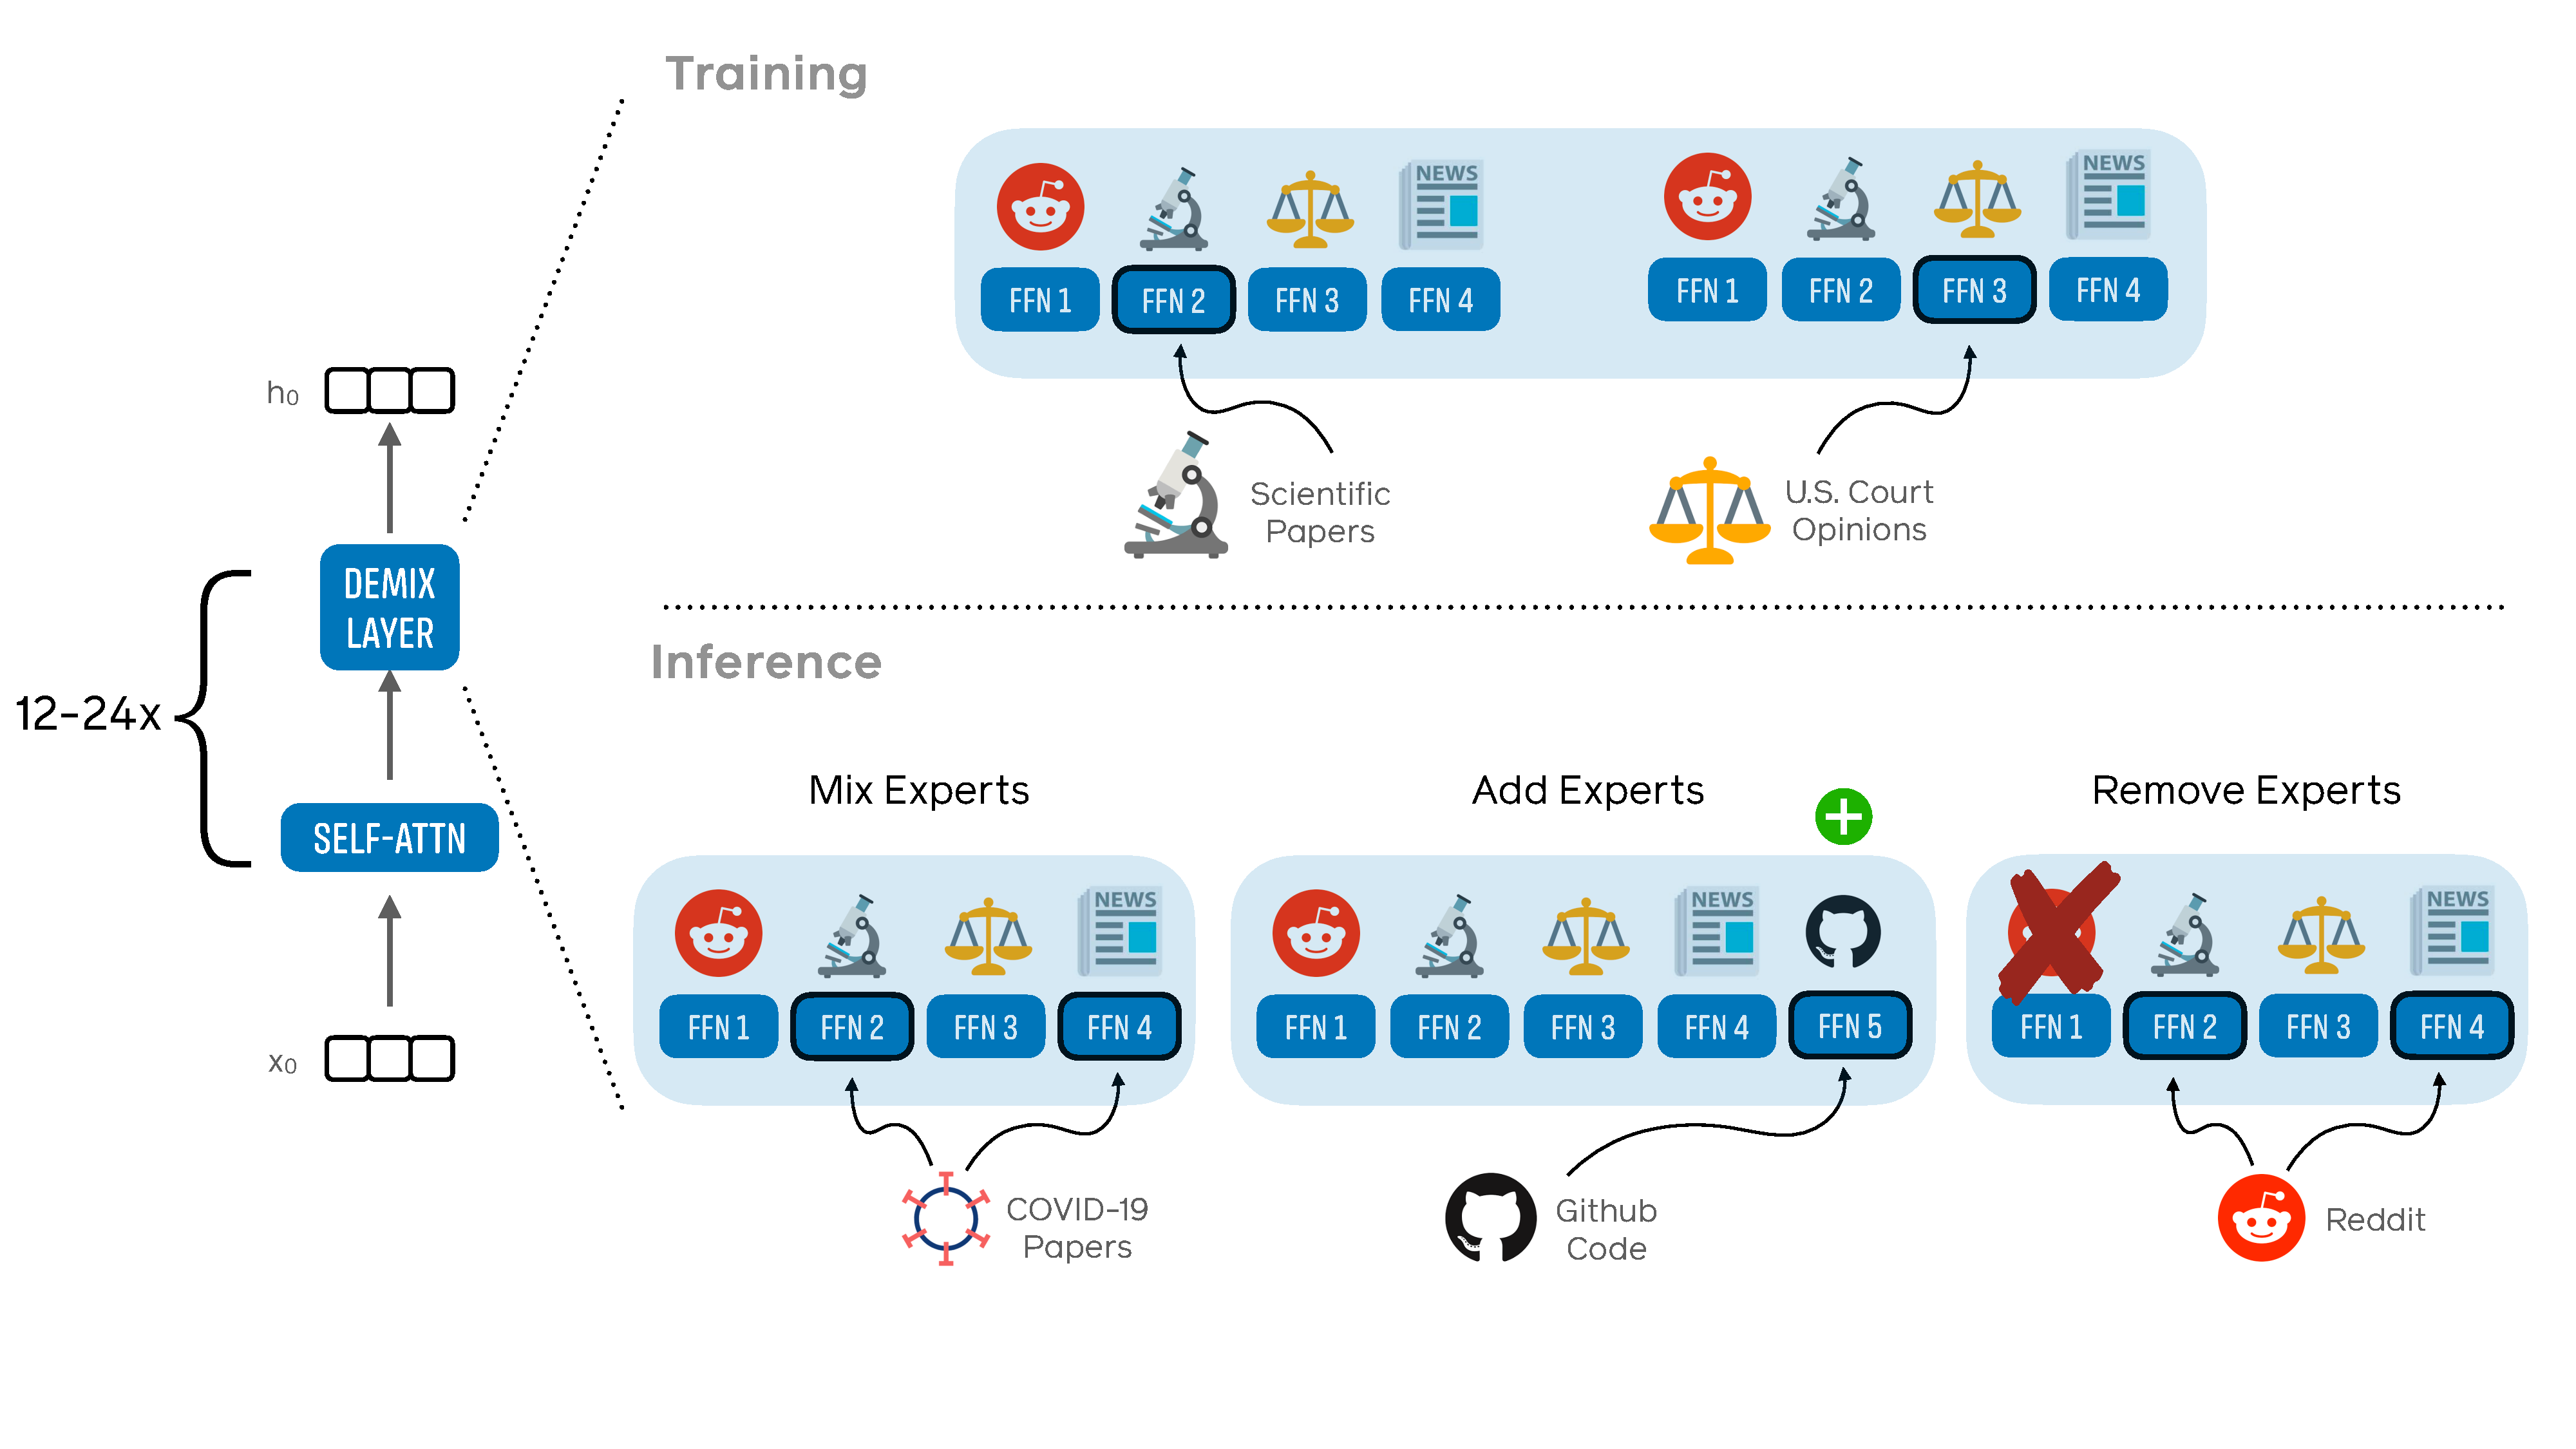
\includegraphics[width=1.0\linewidth]{figures/DEMIX.pdf}
    \caption{DEMix 模型\cite{Gururangan2021DEMixLD}为不同的预训练数据领域显式地分配了不同的专家。}
    \label{fig:DEMIX}
\end{figure}


\paragraph{混合路由策略（Hybrid Routing Strategies）}
为了结合不同规则化路由的优点，研究者们还提出了混合策略。例如，PanGu-$\Sigma$\cite{Ren2023PanGuTT}模型采用了一种两阶段的路由机制（图\ref{fig:hybrid_domain_hash}）：首先，根据词元所属的领域，将其确定性地路由到一个特定的\textbf{专家组}；然后，在该专家组内部，再通过随机选择的方式确定最终处理该词元的单一专家。这种“先按领域分组，再组内随机”的混合策略，既利用了元数据带来的语义引导，又保留了随机路由的简洁性和负载均衡特性。

\begin{figure}[h]
    \centering
    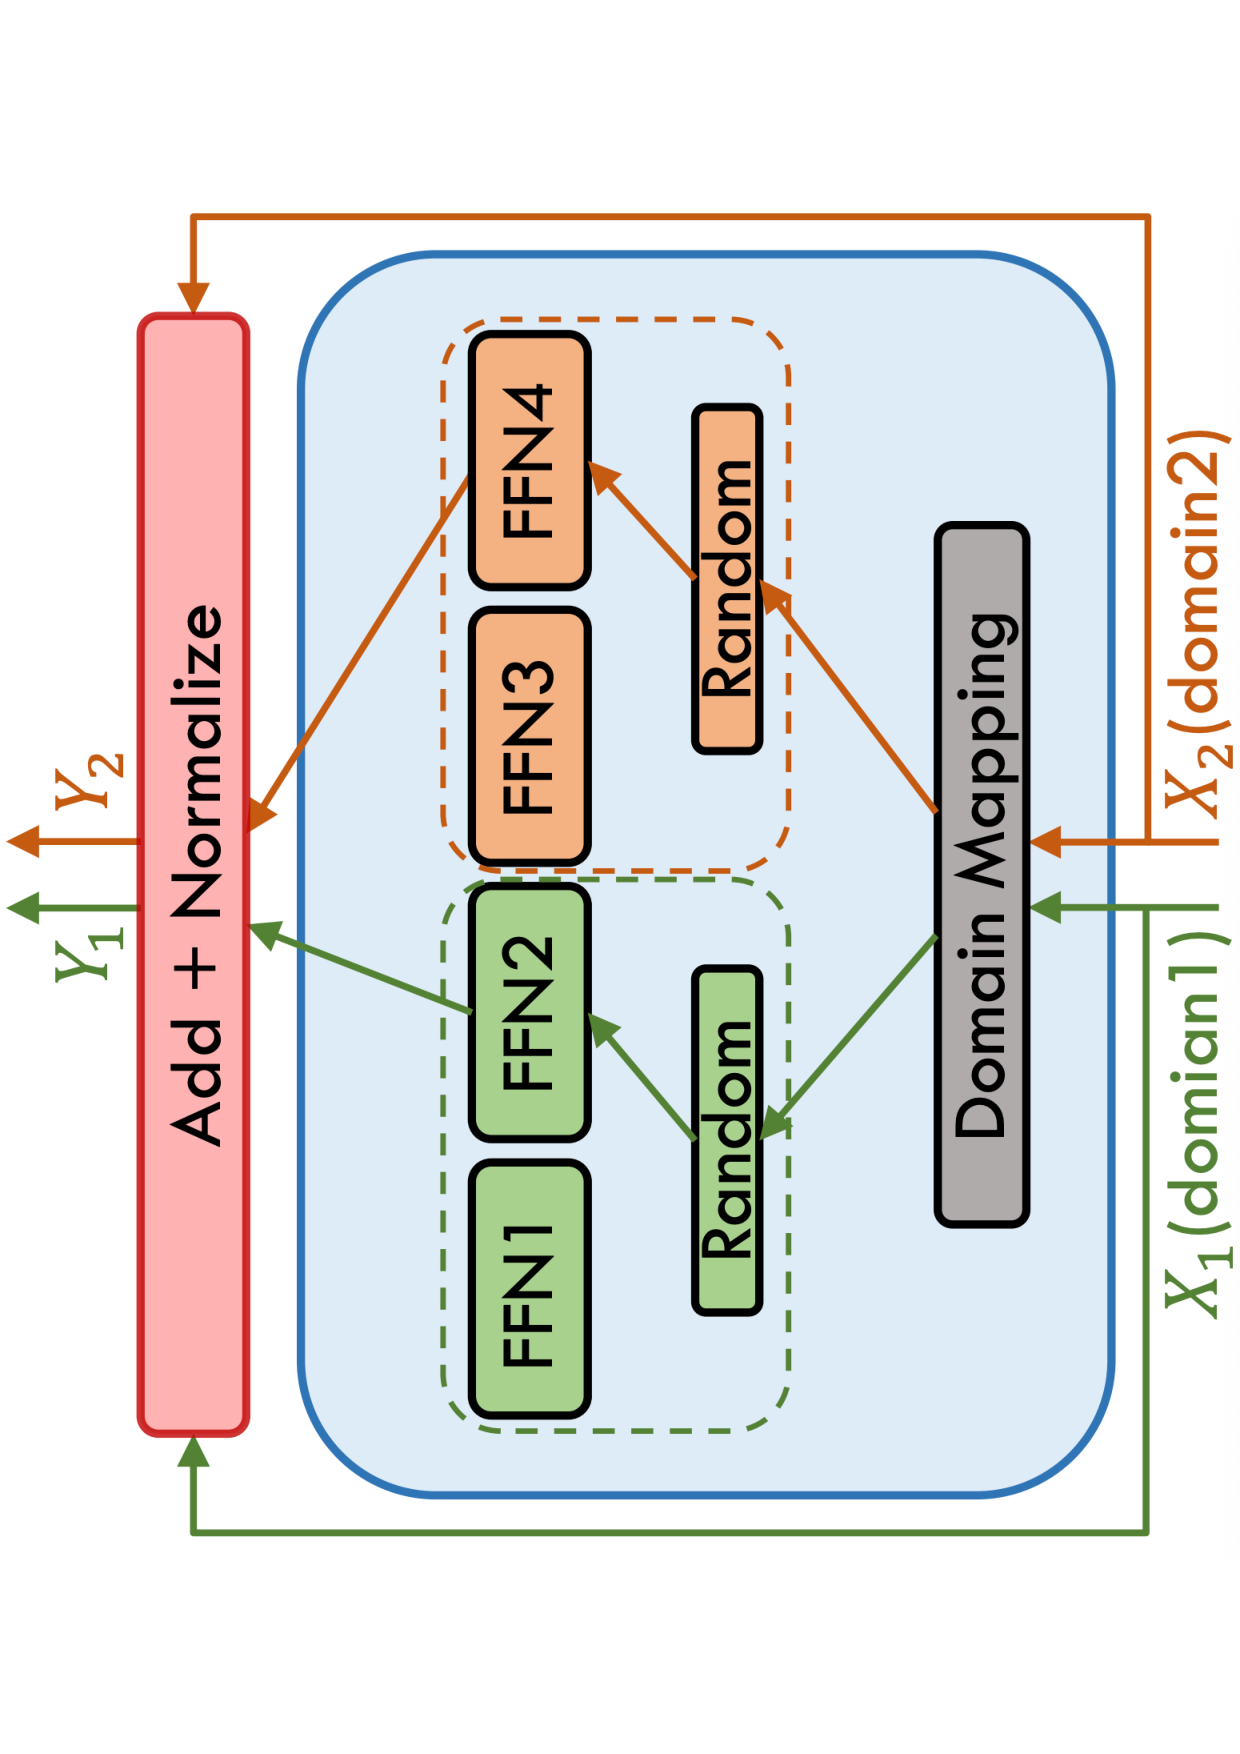
\includegraphics[angle=-90,width=0.8\linewidth]{figures/hybrid_domain_hash.pdf}
    \caption{PanGu-$\Sigma$\cite{Ren2023PanGuTT}模型的两阶段路由机制}
    \label{fig:hybrid_domain_hash}
\end{figure}


从某种意义上说，基于规则的路由相当于使用基于人类先验的路由策略替代了基于数据驱动学习的路由策略。它在特定场景下能够发挥一定的作用，也有着实现简单、负载均衡好的优点。然而，对于当前面临复杂多变应用场景的大语言模型而言，仅依赖此种单一策略恐显不足。

\subsection{路由器的变种}
经典的路由器采用一个简单的线性变换层后接 \text{Softmax}（或Sigmoid） 和 \text{Top-K} 算子来计算门控权重。为了进一步捕捉输入词元与专家功能之间的复杂关系，提升路由决策的质量和模型的整体性能，研究者们探索了多种相对更复杂的路由器的变种。

\paragraph{余弦路由器（Cosine Router）}
研究发现，经典的线性路由器存在一个潜在的严重问题，即\textbf{表示坍缩}（Representation Collapse）\cite{Chi2022OnTR}。具体而言，在线性路由机制下，为了获得较高的路由得分（logits），模型倾向于将输入词元的隐藏表示（hidden representations）推向与路由器权重向量（可视为专家质心）在空间中极为接近的位置。这种优化压力导致所有词元的表示都向少数几个专家质心聚集，失去了多样性和表达能力，从而损害了模型的整体性能。
为了缓解这一问题，Chi 等人提出采用\textbf{余弦路由器}。其核心思想是将路由决策从基于向量点积的亲和度，转变为基于向量方向的余弦相似度。这通过将词元表示和专家嵌入都投影到一个单位超球面上来实现，从而解耦了向量的\textbf{幅值}（magnitude）与路由得分的关系。路由决策仅依赖于两者之间的夹角，而向量的幅值则可以被模型用于编码其他维度的信息，从而保留了表示的多样性。其门控函数 $G(\mathbf{x})$ 的计算过程如下：
\begin{equation}
G(\mathbf{x}) = \text{TopK} \left( \text{softmax} \left( \tau \cdot \frac{(\mathbf{W}_{\text{linear}}\mathbf{x})^T \mathbf{C}}{\|\mathbf{W}_{\text{linear}}\mathbf{x}\| \|\mathbf{C}\|} \right) \right)
\end{equation}
其中，$\mathbf{x}$ 是输入词元的表示，$\mathbf{W}_{\text{linear}}$ 是一个可学习的线性投影矩阵。$\mathbf{C} \in \mathbb{R}^{d_{model} \times N}$ 代表了 $N$ 个专家的可学习嵌入向量。核心计算部分即为投影后的词元表示与各个专家嵌入之间的余弦相似度。$\tau$ 是控制分布锐利度的温度参数。通过这种方式，余弦路由器有效防止了表示坍缩，鼓励模型学习到更具信息量的特征表示，并在领域泛化等任务上展现出一定的优势。

\paragraph{注意力路由器 (Attention Router)}
为了设计一个能够更有效捕捉词元与专家之间亲和度的路由机制，Yuan 2.0-M32 模型\cite{Wu2024Yuan2M}引入了\textbf{注意力路由器}（Attention Router）。如图\ref{fig:attention_router}所示，该设计将标准注意力机制的思想应用于路由过程，取代了简单的线性层，从而实现了更具动态性和语义感知能力的专家选择。其详细工作流程如下：
\begin{enumerate}
    \item \textbf{输入投影}：与标准自注意力模块类似，输入的单个词元表征 $\mathbf{x}$ 首先被线性投影，生成三组d维向量，每组N（专家数目）个，对应于查询（Query）、键（Key）和值（Value）向量：
    \begin{equation}
    \mathbf{Q} = \mathbf{W}_Q \mathbf{x}, \quad \mathbf{K} = \mathbf{W}_K \mathbf{x}, \quad \mathbf{V} = \mathbf{W}_V \mathbf{x}
    \end{equation}
    \item \textbf{注意力计算}：查询（Query）、键（Key）和值（Value）三组向量按照注意力机制计算出一个N维输出向量$\mathbf{P}$，表示该词元与每个专家的相关性：
    \begin{equation}
    \mathbf{P} = \text{softmax}\left(\mathbf{Q} \mathbf{K}^T\right)\mathbf{V}
    \end{equation}
    \item \textbf{专家选择}：选取N维输出向量$\mathbf{P}$中前$K$大的分数对应的专家。
\end{enumerate}
这种设计允许路由器在做出最终路由决策前，进行一次丰富的特征交互。它不仅考虑了词元自身的属性，还动态地融入了该词元与整个专家池的关联信息，从而实现了比简单线性映射更复杂的专家选择。在Yuan 2.0-M32中，$K=2, N=32, d=2048$。

\paragraph{平均键路由器 (Avg-K Router)}
Liu 等人提出\cite{Liu2023TowardsAU}，可以将混合专家模型（MoE）的 Transformer 层看作一个拥有巨大尺寸的、被分块的键值对记忆网络（Key-Value Memory Network）。在这个视角下，每个专家（Expert）本质上是一个独立的记忆块（Memory Block），包含了若干键（Key）和值（Value）向量对，而前馈网络（FFN）的计算过程可以被视为一种记忆检索和整合的过程。一个标准的前馈网络计算可以表示为：
\begin{equation}
    y = \text{FFN}(x) = f(x \cdot K^T) \cdot V
\end{equation}
其中 \(x\) 是输入，\(K\) 和 \(V\) 分别是前馈网络的两个线性层的权重，可以被看作是记忆的键表和值表。
从这个角度出发，经典的混合专家模型路由器在选择专家时，使用的是一个独立于专家内部参数（即键 \(K\)）的门控网络。这种分离可能导致路由决策与专家的实际功能存在偏差。
为了将路由决策与专家的内在功能更紧密地联系起来，Liu 等人提出了 \textbf{Avg-K} 路由方法。该方法直接利用每个专家（记忆块）自身的键向量来决定路由。其核心思想是，用每个记忆块中所有键向量的平均值来代表这个记忆块。具体算法如下：
\begin{enumerate}
    \item \textbf{计算专家代表向量}：对于第 \(i\) 个专家，其代表向量 \(e_i\) 由该专家内部的所有键向量 \(k_j^{(i)}\) 的平均值计算得出。假设每个专家（记忆块）的大小为 \(g\)，则：
    \begin{equation}
        e_i = \text{Avg}(\mathbf{K}^{(i)}, \text{dim=0}) = \frac{1}{g} \sum_{j=0}^{g-1} k_j^{(i)}
    \end{equation}
    其中 \(\mathbf{K}^{(i)}\) 是第 \(i\) 个专家的键矩阵。
    \item \textbf{计算路由得分}：输入词元 \(x\) 与每个专家的代表向量 \(e_i\) 计算点积，得到路由得分。
    \begin{equation}
        \text{score}_i = x \cdot e_i
    \end{equation}
    \item \textbf{专家选择}：根据计算出的得分，选择得分最高的 \(b\) 个专家进行激活。
\end{enumerate}
由于平均操作的线性特性，计算输入 \(x\) 与平均键向量的点积，等价于计算 \(x\) 与该专家内所有键向量的点积然后取平均值。这种设计直接利用了专家的键信息，增强了路由决策的依赖性，从而获得了较好的性能。

\begin{figure}[h]
    \centering
    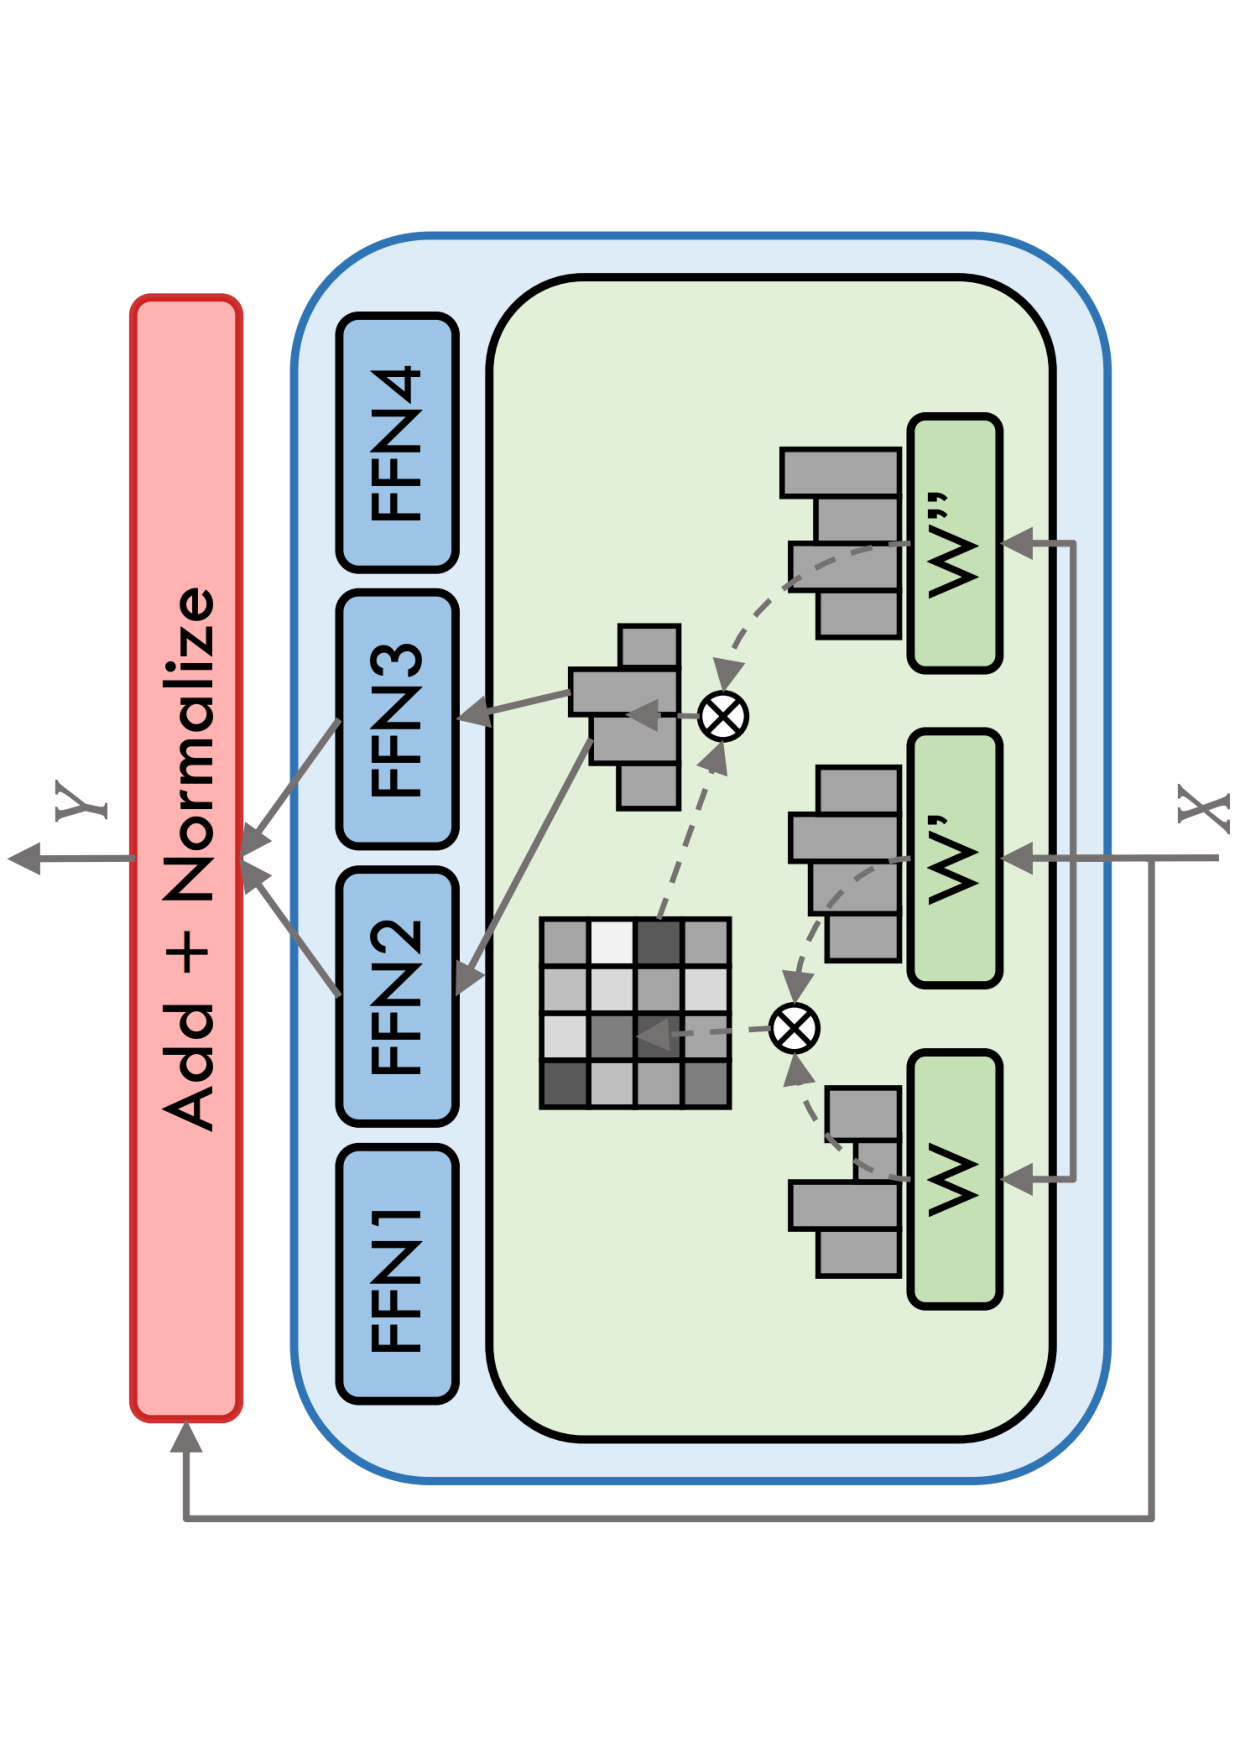
\includegraphics[angle=-90,width=0.8\linewidth]{figures/attention_router.pdf}
    \caption{注意力路由器}
    \label{fig:attention_router}
\end{figure}

\subsection{路由器的学习算法}
\label{sec:router_learning}
路由器的参数 $W_g$ 对于混合专家模型的性能至关重要，因为它直接决定了每个输入词元应该由哪些专家进行处理。然而，如 \ref{sec:classic_top-k} 所述，Top-k 选择操作本身是离散的、不可导的，这为通过标准的反向传播算法来训练路由器带来了挑战。为了解决这个问题，研究者们借鉴了强化学习和数值方法等领域的思想，提出了一系列新颖的学习算法。

\paragraph{REINFORCE 算法及其变种}
REINFORCE\cite{Williams2004SimpleSG}是一种经典的策略梯度方法，常用于优化随机策略网络。在混合专家模型的上下文中，可以将路由器的决策过程视为一个策略：对于给定的输入词元 $x$，路由器选择一个或多个专家的动作\cite{Clark2022UnifiedSL}。REINFORCE 算法的核心思想是通过最大化期望奖励来更新策略参数。
具体来说，REINFORCE 梯度估计器在理论上是无偏的，并且只要求离散变量的分布是可导的，而不需要通过模型的其余部分 $g$ 进行反向传播。其梯度估计的形式如下：
\begin{equation}
\nabla_{\text{REINFORCE}} := g(\pi_D f_D(x)) \frac{\partial \log \pi_D}{\partial W_r}
\end{equation}
其中 $D$ 是被选择的专家，$g(\pi_D f_D(x))$ 可以被看作是选择专家 $D$ 后获得的奖励 (reward)。尽管 REINFORCE 算法在理论上是无偏的，即其梯度估计的期望等于真实的梯度，但它在实践中往往存在高方差的问题。
为了解决 REINFORCE 算法固有的高方差问题，研究者们提出了一系列基于控制变量 (control variates) 的改进方法。这些方法的核心思想是从原始的梯度估计中减去一个期望为零的随机变量，从而在不改变梯度期望（保持无偏性）的前提下，有效降低其方差。例如，MuProp\cite{Gu2015MuPropUB}使用了基于函数泰勒展开的控制变量；REBAR\cite{Tucker2017REBARLU}则巧妙地将低方差但有偏的估计器与 REINFORCE 相结合，构建出一个既无偏又低方差的梯度估计器；Grathwohl等人\cite{Grathwohl2017BackpropagationTT}更是提出通过训练一个独立的神经网络来学习最优的控制变量，以最大程度地降低方差。

\paragraph{SparseMixer 算法}
为了克服梯度直通估计 (Straight-Through Estimator, STE) 需要密集计算所有专家输出的限制，同时为被忽略的梯度项提供更可靠的估计，Liu 等人提出了 SparseMixer 算法\cite{liu2023sparsebackpropagationmoetraining}。该算法基于数值常微分方程 (ODE) 求解器的思想，旨在以一种可扩展的方式，为路由器提供更精确的梯度近似，且计算开销较小。SparseMixer 的核心思想是将路由器的梯度计算问题重新构建为一个数值积分问题。具体来说，损失函数关于路由器参数的梯度可以分为两部分 $\nabla_0$ 和 $\nabla_1$。其中 $\nabla_1$ 可以通过标准的反向传播计算，而 $\nabla_0$ 包含了与路由概率 $\pi$ 相关的项，这部分梯度的计算是难点所在。SparseMixer 提供了一种有效的方法来近似 $\nabla_0$。该算法利用了二阶 ODE 求解器，特别是中点法 (mid-point method)，来提供比传统一阶方法（如前向欧拉法，这可以看作是 STE 的一种理论解释）更精确的梯度近似。SparseMixer 的二阶版本（SparseMixer-2nd）的梯度估计形式如下：
\begin{equation}
\nabla_{\text{SparseMixer-2nd}} := 2 \cdot \frac{\partial g(\frac{\pi_D}{2} f_D(x))}{\partial W_r}
\end{equation}
其中，$D$ 是被选择的专家，$f_D(x)$ 是其输出，$g(\cdot)$ 代表模型的其余部分，$\pi_D$ 是路由到该专家的概率，$W_r$是路由器的线性变换矩阵。 这种方法在不引入 Hessian 矩阵或其他二阶导数的情况下，达到了二阶精度，并且重要的是，它只需要被激活专家的输出，从而保持了计算的稀疏性。在Liu等人的实验中，将 SparseMixer 应用于 Switch Transformer 等模型，可以显著提升性能，将训练收敛速度提升两倍。

\paragraph{Router z-loss}
在改进梯度估计算法本身以外，Zoph 等人在其 ST-MoE 的工作中提出了一种名为“Router z-loss”的辅助损失\cite{Zoph2022STMoEDS}，旨在控制路由器输出的 logits 的范围，避免logits位于浮点数精度较低的区间（也就是浮点数绝对值过大的位置）。其定义如下：
\begin{equation}
L_z = \frac{1}{T} \sum_{t=1}^{T} (\log \sum_{i=1}^{N} e^{h_i(x_t)})^2
\end{equation}
其中 $T$ 是批次中的词元总数，$N$ 是专家数量，$h_i(x_t)$ 是路由器为第 $t$ 个词元分配给第 $i$ 个专家的 logit。
这个损失函数会惩罚那些具有较大幅度的 logits，因为它会促使 $\sum e^{h_i(x_t)}$ 的值变大。在较大规模的混合专家模型上，这一辅助损失有利于促进训练稳定性。

\paragraph{两阶段稳定路由策略 (StableMoE)}
StableMoE\cite{Dai2022StableMoESR}认为，依赖学习的路由方法普遍存在\textbf{路由抖动 (routing fluctuation)} 的问题，即在训练过程中，同一个输入词元在不同阶段会被分配给不同的专家。这种不稳定性损害了样本效率，因为模型在多个专家上更新了参数，但在推理时仅使用最终确定的一个专家。为了解决此问题，StableMoE提出了一种两阶段训练策略，旨在学习一个稳定且高效的路由策略（图\ref{fig:stable_moe}）。
\begin{itemize}
    \item \textbf{第一阶段：学习与蒸馏}。在此阶段，模型采用标准的“学习路由”范式，通过优化任务损失和负载均衡损失来训练一个路由策略。与此同时，模型将这个动态学习到的、依赖于骨干网络深度表征的路由策略，通过\textbf{知识蒸馏 (knowledge distillation)} 的方式，提炼到一个与骨干网络解耦的、轻量级的\textbf{蒸馏路由器 (distilled router)}中。这个轻量级路由器通常仅使用词元的浅层表征（如词嵌入）作为输入，其学习目标是模仿主路由器的路由决策。此阶段的总损失函数为：
    $$ L_{S1} = L_{task} + L_{bal} + L_{dis} $$
    其中 $L_{task}$ 是主任务损失，$L_{bal}$ 是负载均衡损失，$L_{dis}$ 是蒸馏损失（通常为交叉熵）。
    \item \textbf{第二阶段：基于稳定路由的学习}。在第一阶段结束后，将蒸馏路由器的参数\textbf{冻结}。在整个第二阶段的训练中，所有词元的专家分配完全由这个固定的、轻量级的路由器决定。由于路由策略不再变化，路由抖动问题被彻底消除。此时，模型不再需要负载均衡和蒸馏损失，训练目标仅为主任务损失：
    $$ L_{S2} = L_{task} $$
\end{itemize}
这种两阶段方法通过先学习再固化的方式，成功地为混合专家模型提供了一个稳定、一致的路由机制，在保证路由质量的同时，提升了训练的稳定性和最终的模型性能。

\begin{figure}[h]
    \centering
    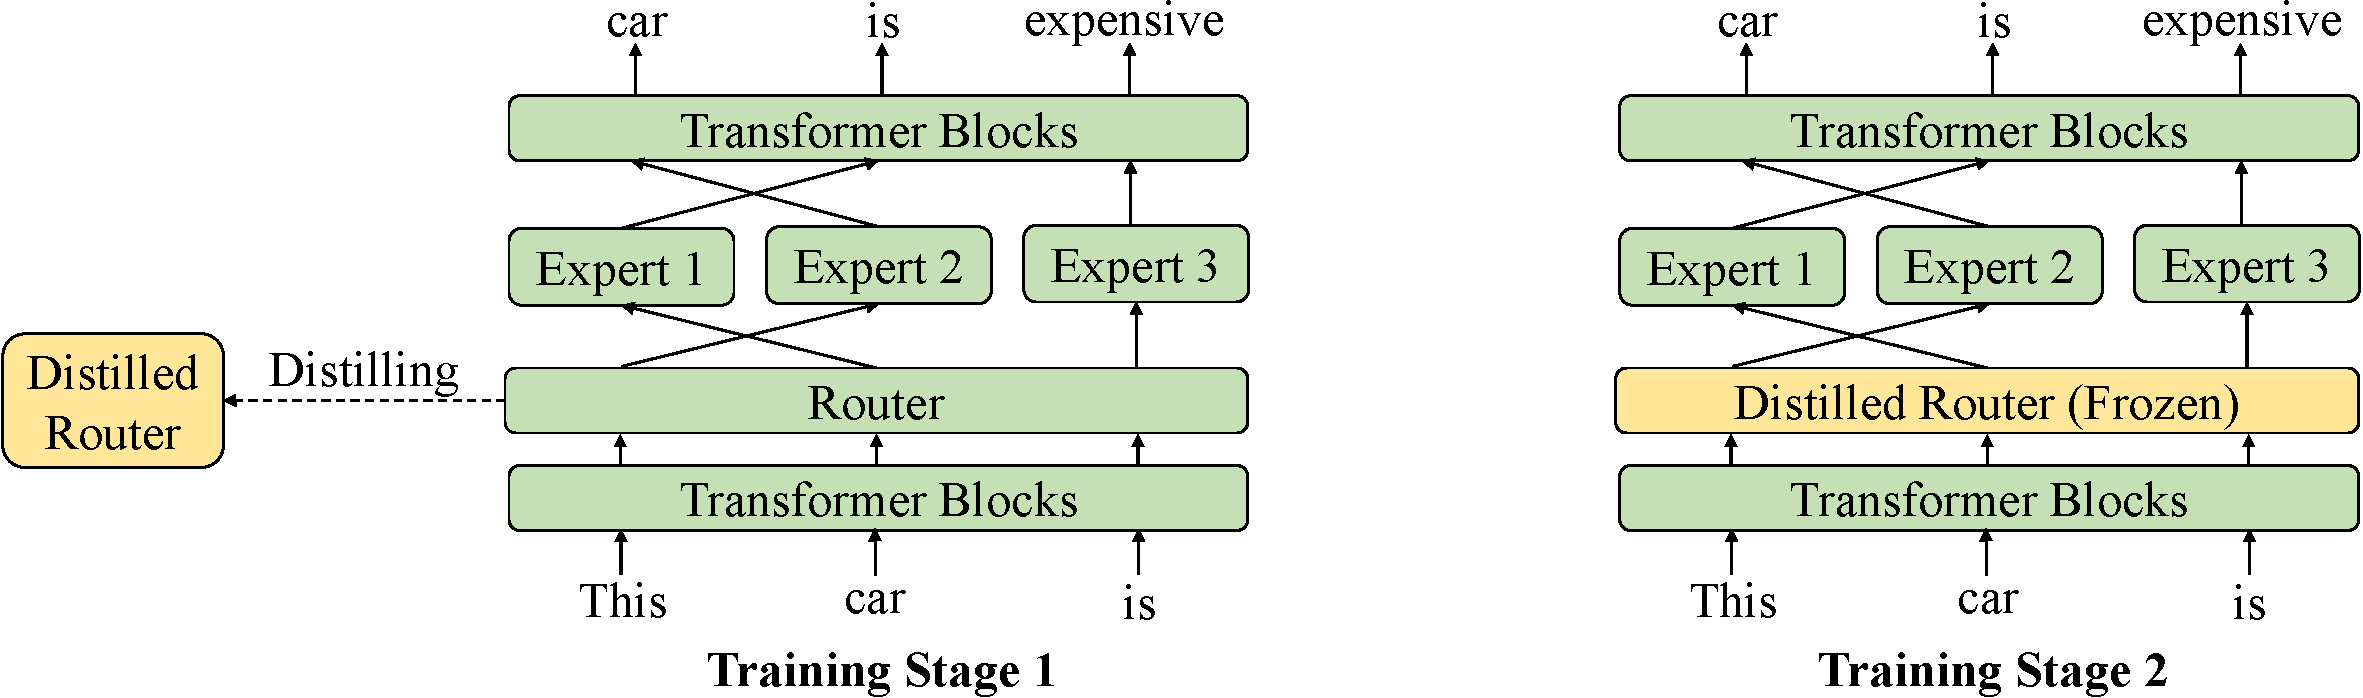
\includegraphics[width=1.0\linewidth]{figures/stable_moe.pdf}
    \caption{StableMoE的两阶段路由策略\cite{Dai2022StableMoESR}}
    \label{fig:stable_moe}
\end{figure}

\paragraph{专家自主路由 (Autonomy-of-Experts, AoE)}
经典路由机制的一个核心挑战是\textbf{决策与执行的分离}\cite{Lv2025AutonomyofExpertsM}：路由器负责预测哪个专家最适合处理输入，但它无法直接评估专家处理该输入的实际能力。这种分离可能导致次优的专家选择。
为了解决这一根本性问题，专家自主路由 (Autonomy-of-Experts, AoE)\cite{Lv2025AutonomyofExpertsM} 提出了一种全新的范式：\textbf{移除独立的路由器，让专家自主决定是否处理输入}（图\ref{fig:AOM}）。其核心思想是，一个专家对其自身处理特定词元的能力是有感知的，这种感知体现在其内部的激活向量的范数上。
具体机制如下：
\begin{enumerate}
    \item \textbf{初步计算与激活评估}。对于每个输入词元 $x$，MoE层中的\textit{所有}专家都对其执行一个低成本的初步前向计算。然后，基于该计算得到的激活的\textbf{范数}（如 L2 范数）来评估每个专家的“胜任度”。激活范数越大，代表该专家被该输入“激活”的程度越高，也就越适合处理它。

    \item \textbf{自主选择与执行}。根据所有专家的激活范数对它们进行排序，只有排名最高的$K$个专家会继续完成剩余的计算流程，而其他专家则中止计算。最终的输出由这$K$个被激活专家的结果加权组合而成。
\end{enumerate}
为了保证初步计算的效率，AoE采用了\textbf{权重矩阵的低秩分解 (low-rank factorization)}。例如，专家的第一个前馈网络权重 $W_1$ 被分解为两个低秩矩阵 $W_{down} \in \mathbb{R}^{d_{model} \times d_{low}}$ 和 $W_{up} \in \mathbb{R}^{d_{low} \times d_{ffn}}$。这样，第 $i$ 个专家的选择分数 $p_i$ 可以高效地计算：
$$ p_i = \left\| x W_{down, i} \right\|_2 $$
其中 $x W_{down, i}$ 的计算开销远小于完整的 FFN 计算。被选中的专家可以复用这个已经计算出的低维激活，继续后续的计算。
通过这种方式，AoE将路由决策权交还给专家自身，使其基于实际的内部状态进行自主选择，从而实现了更精准的专家分配和更有效的学习。


\begin{figure}[h]
    \centering
    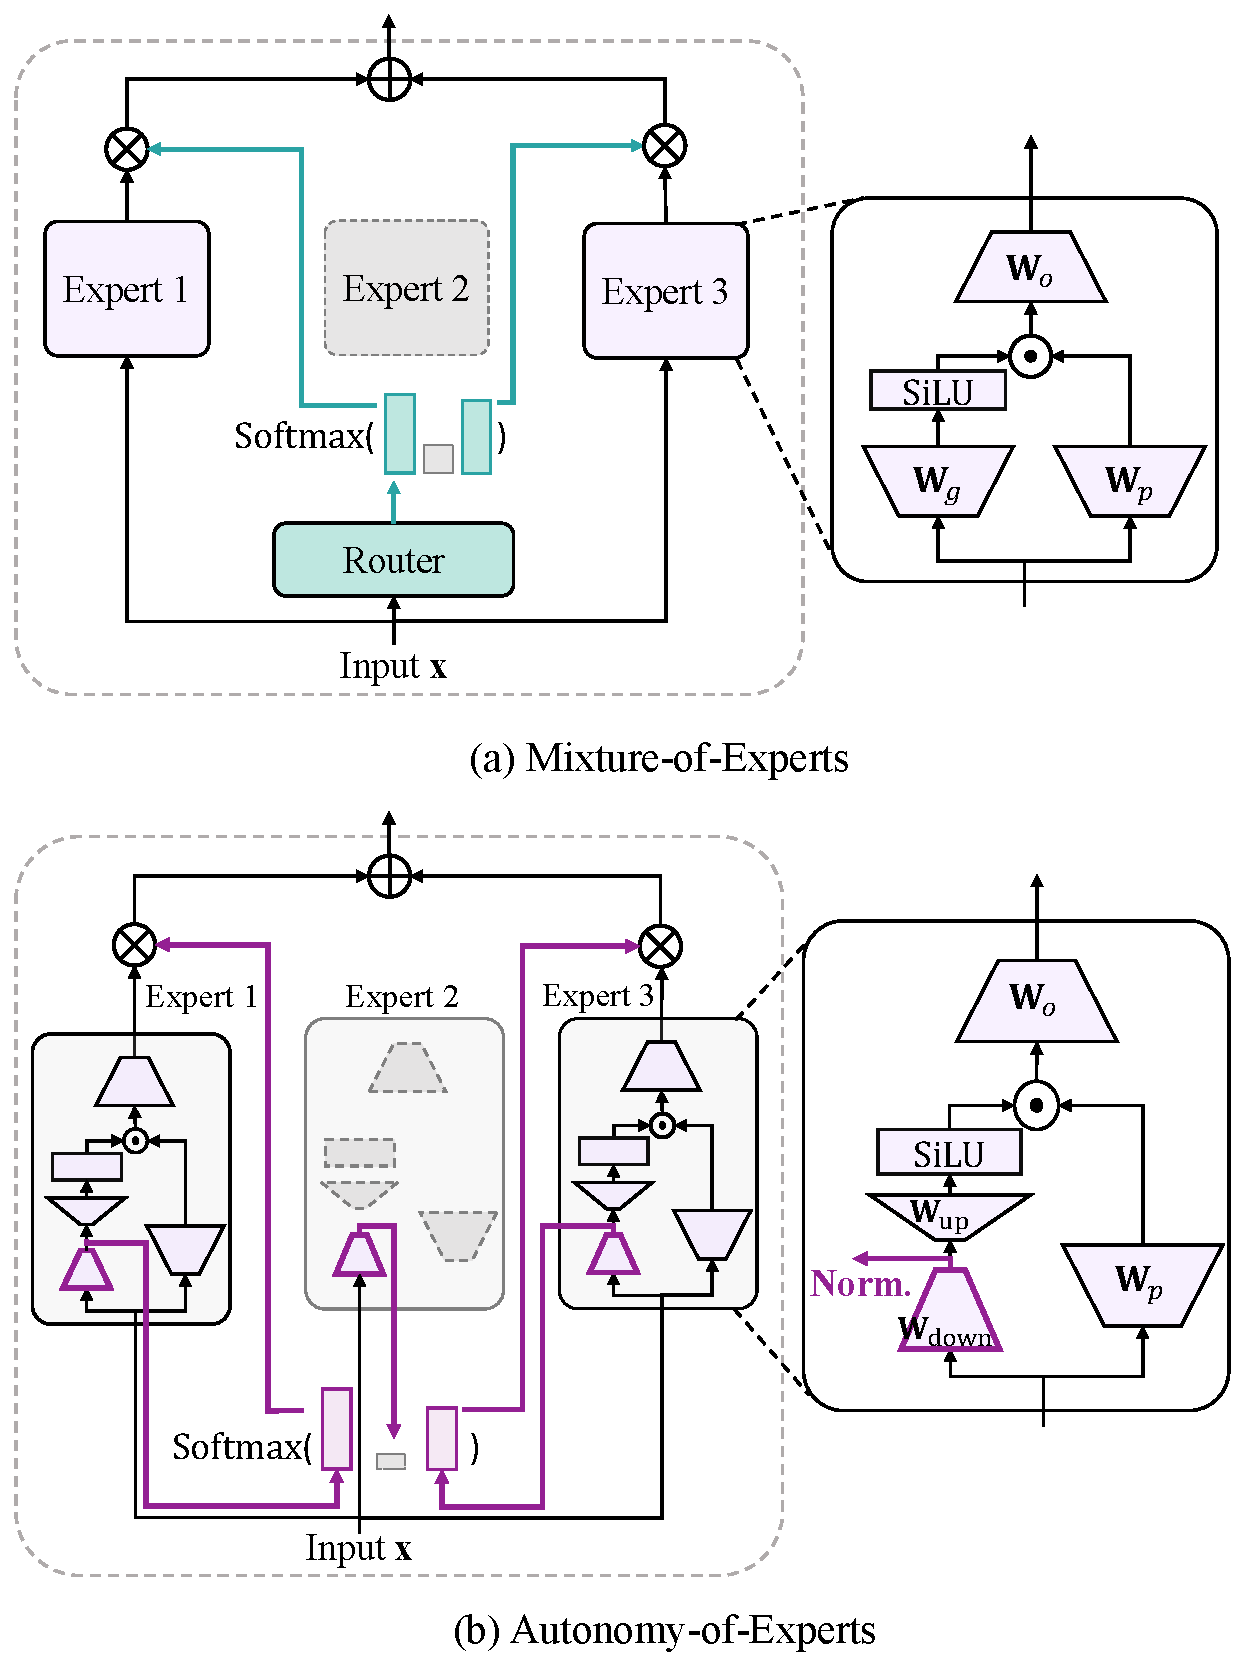
\includegraphics[width=0.7\linewidth]{figures/AOM.pdf}
    \caption{AOE与普通混合专家模型的对比\cite{Lv2025AutonomyofExpertsM}}
    \label{fig:AOM}
\end{figure}

\subsection{异构专家设计 (Heterogeneous Expert Design)}
经典的混合专家模型通常采用同质专家网络（Homogeneous Experts），即所有专家的网络结构和参数量都相同。然而，输入序列中的不同词元的计算复杂性存在差异，使用相同规模的专家处理所有词元可能导致计算资源的次优分配。为了解决这一问题，近期研究开始探索异构专家设计，通过引入不同类型或规模的专家来提升模型的效率和性能。

\paragraph{\raisebox{0.05ex}{\scalebox{0.96}{$\mathbf{\mathcal{A}}$}}\textit{da}\raisebox{0.04ex}{\textsc{\scalebox{0.85}{MoE}}}\xspace}
为了实现更灵活的路由机制，\raisebox{0.05ex}{\scalebox{0.96}{$\mathbf{\mathcal{A}}$}}\textit{da}\raisebox{0.04ex}{\textsc{\scalebox{0.85}{MoE}}}\xspace\cite{Zeng2024AdaMoETR} 提出了\textbf{空专家} (Null Experts) 的概念。其核心思想是在原有的 $n$ 个“真”专家之外，额外增加 $m$ 个空专家（图\ref{fig:adamoe}）。空专家的计算过程是一个恒等或零映射，不产生任何计算开销（FLOPs）。同时，路由器的 Top-k 选择机制中的 $k$ 值被放大到一个更大的值 $k' (k' > k)$。这样，当一个词元被路由时，其选择的 $k'$ 个专家中可能包含若干空专家。最终，该词元实际只由被选中的真专家处理，从而实现了每个词元可以自适应地激活可变数量的真专家，打破了传统混合专家模型中每个词元必须激活固定$k$个专家的限制。

\begin{figure}[h]
    \centering
    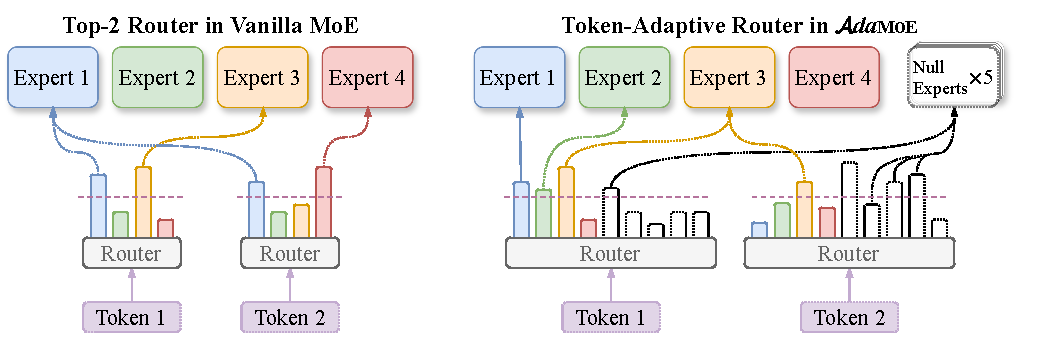
\includegraphics[width=1.0\linewidth]{figures/admoe.pdf}
    \caption{{\raisebox{0.05ex}{\scalebox{0.96}{$\mathbf{\mathcal{A}}$}}\textit{da}\raisebox{0.04ex}{\textsc{\scalebox{0.85}{MoE}}}\xspace}的示意图\cite{Zeng2024AdaMoETR}}
    \label{fig:adamoe}
\end{figure}

\paragraph{MoE++}
MoE++ \cite{Jin2024MoEAM} 框架（图\ref{fig:moe++}）引入了更丰富的\textbf{零计算专家} (Zero-Computation Experts) 来实现灵活的计算分配。具体包括三种类型：(1) \textbf{零专家 (Zero Expert)}，直接丢弃输入，输出为零向量；(2) \textbf{拷贝专家 (Copy Expert)}，直接复制输入作为输出，功能类似于残差连接；(3) \textbf{常数专家 (Constant Expert)}，用一个可训练的向量替换输入。这些设计使得简单的词元可以选择计算开销极低的路径，而将宝贵的前馈网络专家资源留给更复杂的词元。此外，MoE++还引入了\textbf{门控残差} (Gating Residuals) 机制，将上一层的路由分数作为当前层路由计算的一部分，使得路由决策能够感知词元在网络中的历史路径。

\begin{figure}[h]
    \centering
    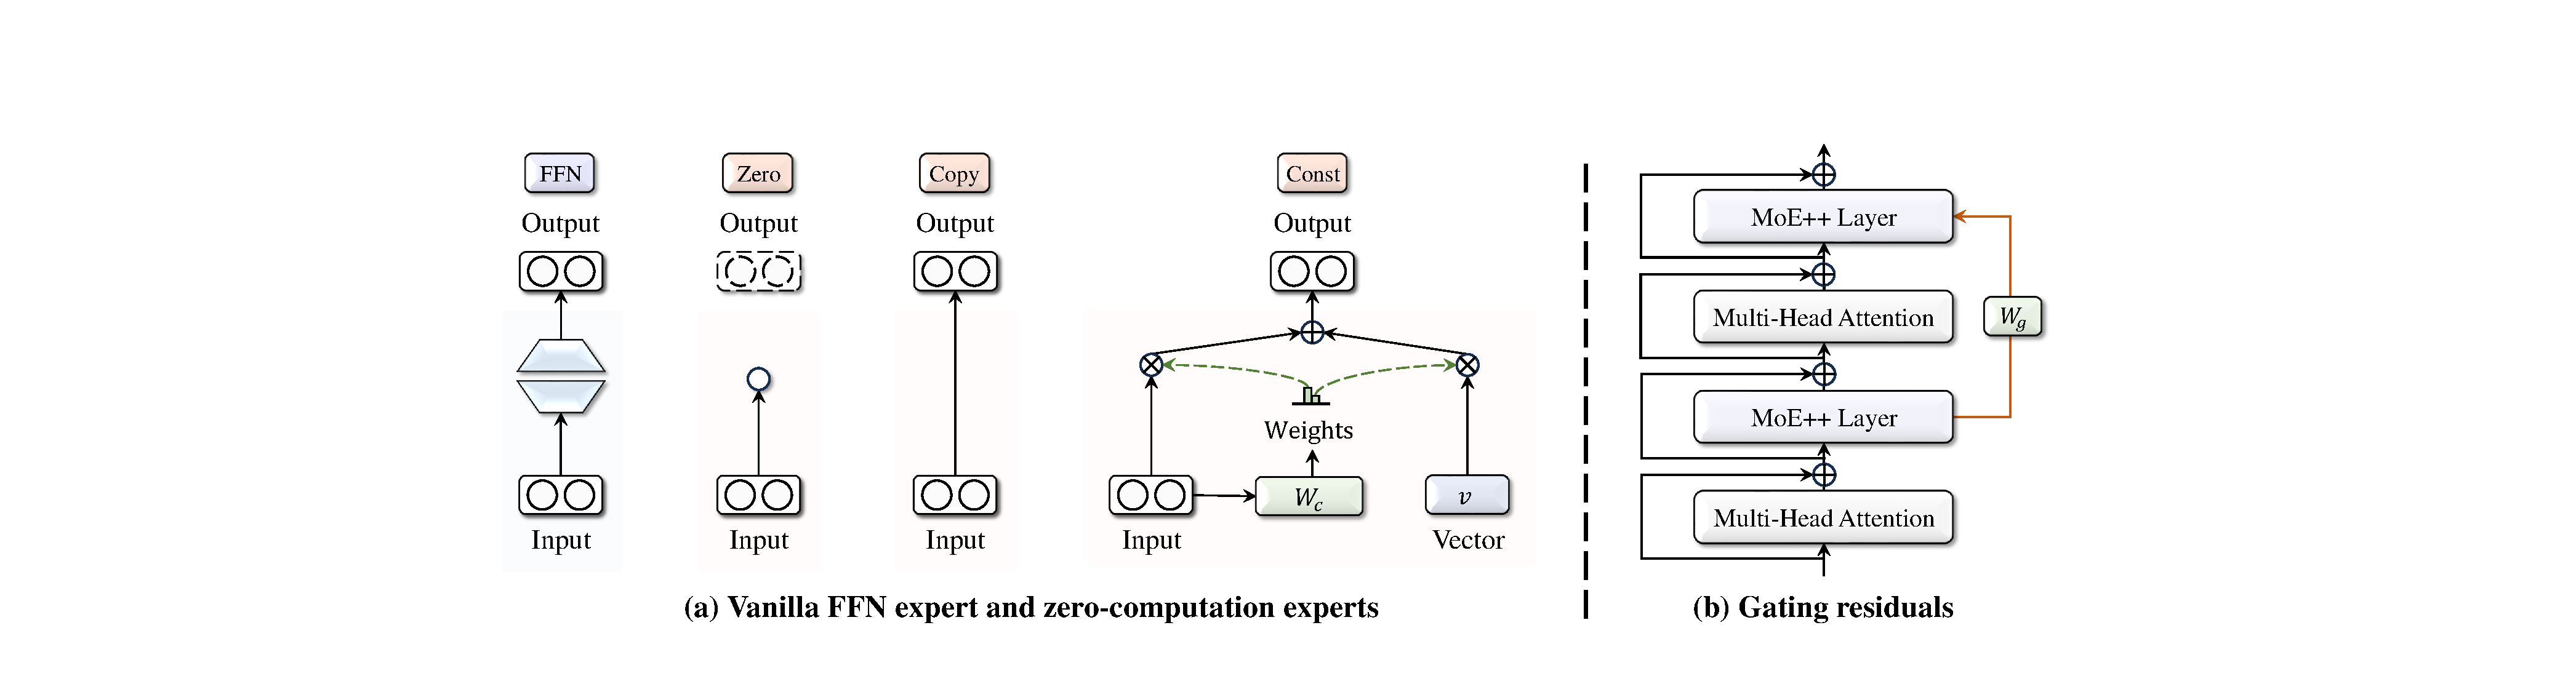
\includegraphics[width=1.0\linewidth]{figures/moe++.pdf}
    \caption{MoE++中的（a）不同类型专家和（b）门控残差机制的示意图\cite{Jin2024MoEAM}}
    \label{fig:moe++}
\end{figure}

\paragraph{HMoE}
HMoE (Heterogeneous Mixture of Experts) \cite{Wang2024HMoEHM} 模型为每个专家设置了不同的隐藏层维度，从而构建了大小各异的专家网络（图\ref{fig:hmoe}）。其核心思想是，让模型能够为复杂的词元分配计算能力更强的大专家，而为简单的词元分配计算开销较小的小专家。然而，这种设计面临一个挑战：在训练过程中，模型会倾向于频繁激活性能更优的大专家，导致小专家得不到充分训练。为解决此问题，HMoE 引入了一种新的\textbf{参数惩罚损失} (Parameter Penalty Loss)，在经典的负载均衡损失基础上，根据专家的大小对其激活进行加权惩罚。该损失函数的形式如下：
\begin{equation}
    L_{\text{P-Penalty}} = N \sum_{i=1}^{N} M_i \cdot P_i
\end{equation}
其中，$M_i$ 是专家 $i$ 在整个批次中被激活的频率乘以隐藏层维度，$P_i$ 是专家 $i$ 从路由器获得的平均门控权重。该损失函数会惩罚对大专家的过度激活，引导模型更经济地使用小专家，从而在专家之间形成更高效的功能分化。

\begin{figure}[h]
    \centering
    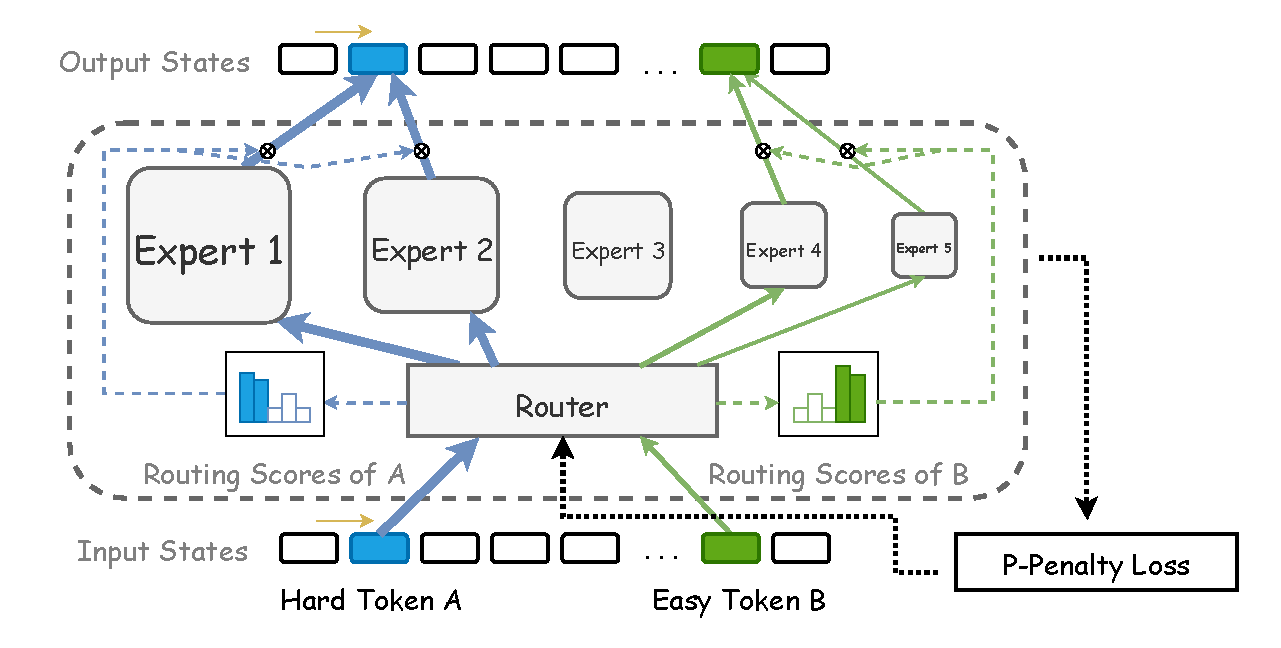
\includegraphics[width=0.9\linewidth]{figures/hmoe.pdf}
    \caption{HMoE模型为每个专家设置了不同的隐藏层维度\cite{Wang2024HMoEHM}。}
    \label{fig:hmoe}
\end{figure}

\paragraph{Grove MoE}
受到CPU计算架构中 big.LITTLE 设计的启发，Grove MoE\cite{Wu2025GroveMT}提出了一种新颖的专家组织方式（图\ref{fig:grovemoe}）。它将 $n$ 个基础专家分为 $g$ 个组，并为每个组分配一个共享的\textbf{伴随专家} (Adjugate Expert) $A_j$。当一个词元激活了某个组内的专家 $E_i$ 时，其最终输出由基础专家和其所在组的伴随专家的输出加权构成：
\begin{equation}
    \tilde{e}_i(x) = E_i(x) + \lambda A_j(x), \quad \text{其中 } E_i \in G_j
\end{equation}
这种设计的关键优势在于其动态计算分配机制。如果一个词元同时激活了同一组内的多个专家，那么共享的伴随专家 $A_j$ 的计算结果会被复用，只需计算一次。这种结构在不显著增加计算复杂度的前提下，高效地扩展了模型容量。此外，为了维持专家间的负载均衡，Grove MoE采用了\textbf{无辅助损失的负载均衡策略} (auxiliary-loss-free load balancing strategy)\cite{Wang2024AuxiliaryLossFreeLB,DeepSeekAI2024DeepSeekV3TR}。该方法不向总损失函数中添加负载均衡惩罚项，而是为每个专家的路由分数引入一个动态偏置项 (dynamic bias term)，通过直接更新该偏置项来最小化专家负载的不均衡，从而实现高效的训练。

\begin{figure}[h]
    \centering
    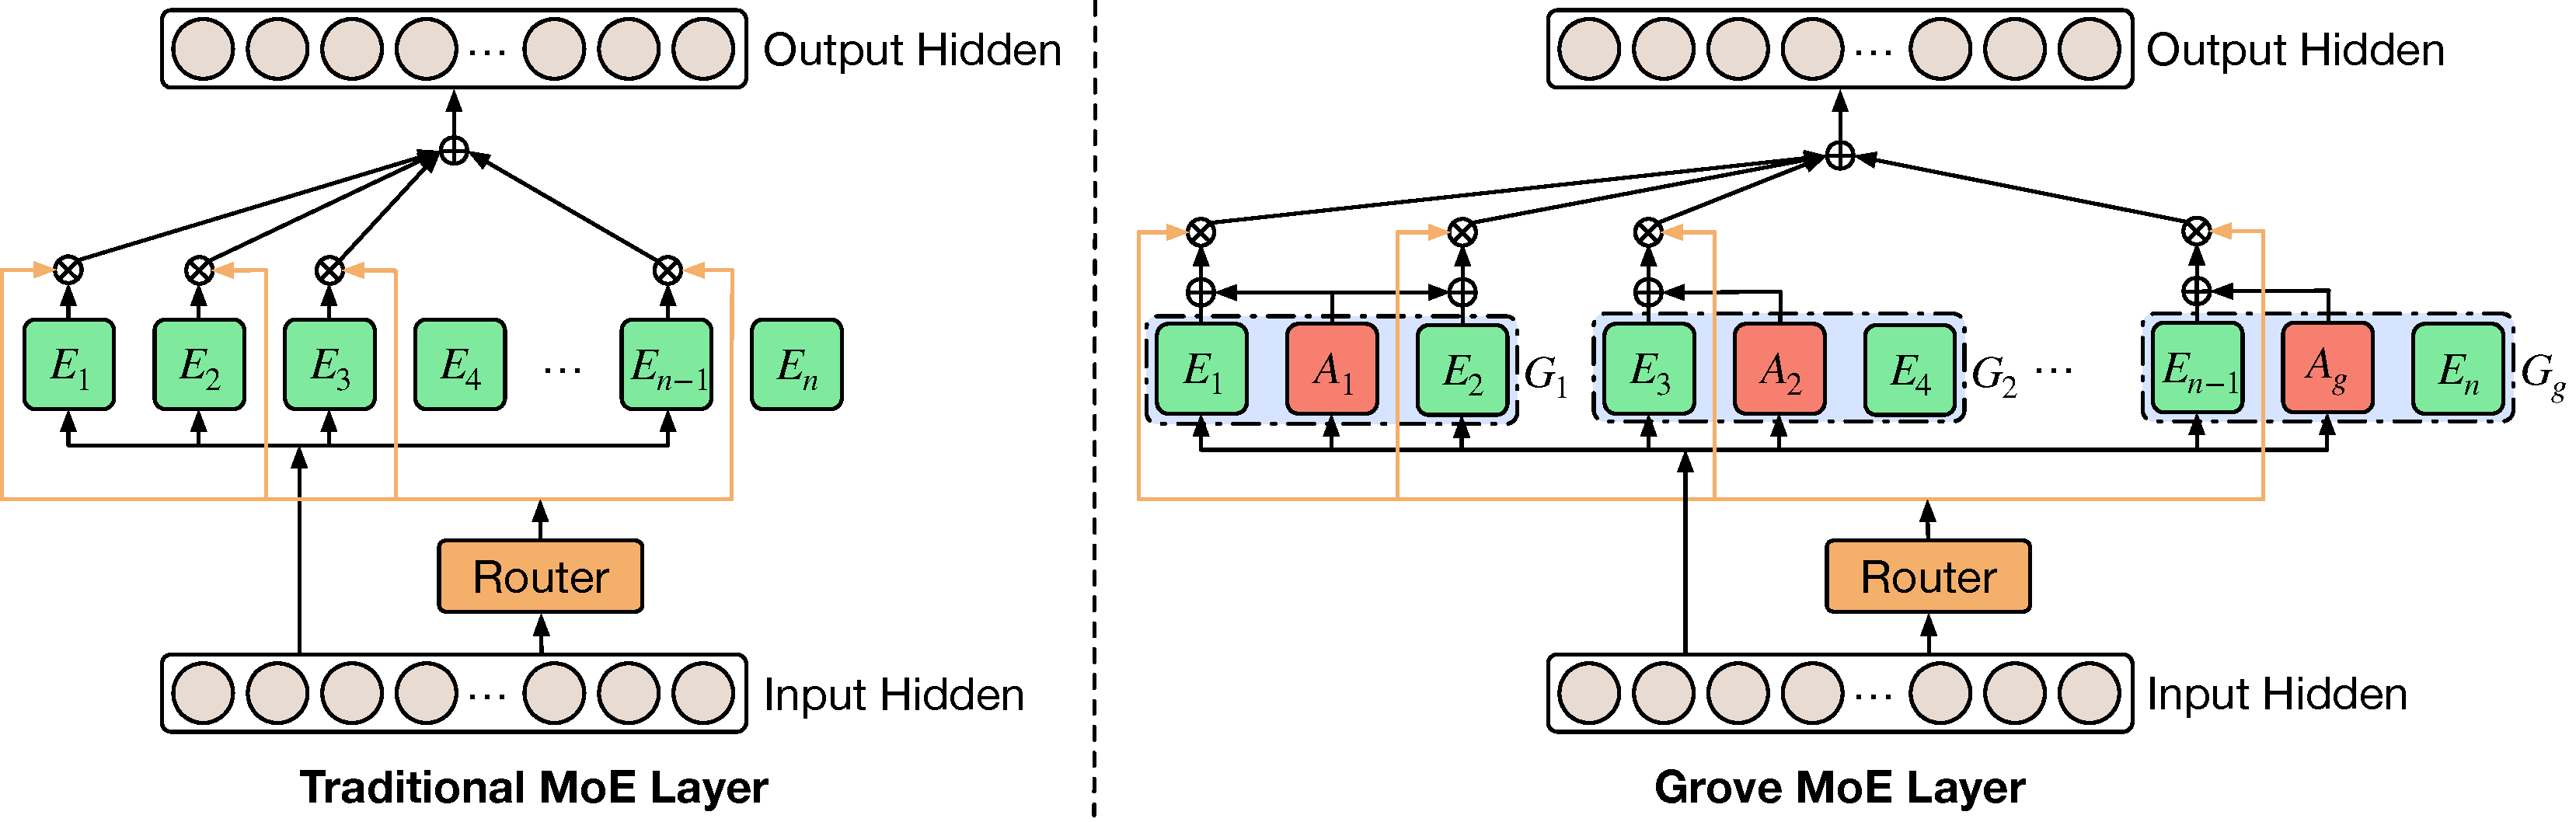
\includegraphics[width=1.0\linewidth]{figures/grovemoe.pdf}
    \caption{Grove MoE的架构\cite{Wu2025GroveMT}}
    \label{fig:grovemoe}
\end{figure}

% \section{专家网络的设计与约束}

% 这部分移到下面去，然后把帐结名字改成负混合专家模型的负载均衡

% aux loss那里提一下global aux loss的问题（引用deepseek v3, 还有阿里的那篇） 均衡性可以参考Aria里的图片，还有deepseek v3的

% 上面的部分补充图片

% \subsection{专家类型与同质性}
% 在当前主流的MoE模型中，如GShard\cite{·}、Switch Transformer\cite{Fedus2021}和Mixtral\cite{Jiang2023}，专家网络通常是\textbf{同质的}（Homogeneous）。这种设计的优势在于实现简单，易于利用专家并行（Expert Parallelism）进行分布式训练。模型的强大能力源于这些结构相同但参数独立的专家在海量数据上训练后，逐渐学习并形成了功能上的\textbf{专业化}（Specialization），这一点将在第五章详细讨论。

% \subsection{专家容量 (Expert Capacity)}
% 在硬件（如GPU/TPU）上高效地实现动态路由存在挑战，因为不同专家处理的词元数量在每个批次中是动态变化的，这会导致计算资源的闲置和同步开销。为了实现静态的计算图和高效的并行计算，GShard\cite{Lepikhin2020}引入了\textbf{专家容量}（Expert Capacity）这一关键的工程约束。专家容量定义了在单个前向传播批次中，每个专家能够处理的词元数量的上限。其计算方式通常为：
% \begin{equation}
%     \text{Capacity} = \left( \frac{\text{Tokens per batch}}{\text{num\_experts}} \right) \times \texttt{capacity\_factor}
% \end{equation}
% 其中，\texttt{capacity\_factor}是一个超参数（通常在1.25到2.0之间），用于为路由不均提供一定的缓冲空间。如果路由到一个专家的词元数量超过了其容量，那么多余的词元将被\textbf{丢弃}（Dropped）。这些被丢弃的词元不经过专家网络计算，其在MoE层的输出通过残差连接（Residual Connection）直接等于其输入。过高的词元丢弃率会损害模型性能，因此设计有效的负载均衡策略以最小化词元丢弃率，是MoE模型训练中的一个核心优化目标。

% \section{MoE模型的训练策略}

% \subsection{核心挑战：负载不均衡}
% 如前所述，MoE模型训练中最核心的挑战是\textbf{负载不均衡}（Load Imbalance）。在没有干预的情况下，Top-k路由器倾向于将大量词元发送给少数几个专家，形成一种“富者愈富”的马太效应。这种现象会导致训练效率低下、模型性能受损，以及大量专家参数得不到充分训练，造成模型容量的浪费。

% \subsection{经典的负载均衡策略：辅助损失函数}
% 为了缓解负载不均衡问题，Shazeer等人\cite{Shazeer2017}提出引入一个\textbf{辅助损失函数}（Auxiliary Loss Function），该方法被后续工作广泛采用。这个损失函数被加权后添加到模型的总损失中，专门用于惩罚不均衡的路由决策。对于一个包含 $T$ 个词元的批次，定义 $f_i$ 为路由到专家 $i$ 的词元比例，$\bar{P}_i$ 为专家 $i$ 从路由器获得的总门控权重之和。辅助损失 $L_{\text{aux}}$ 可以表示为：
% \begin{equation}
%     L_{\text{aux}} = \alpha \cdot \sum_{i=1}^{N} (f_i \cdot \bar{P}_i)
%     \label{eq:aux_loss}
% \end{equation}
% 这个损失函数通过最小化每个专家的词元分配比例和总路由权重的点积，来鼓励路由器将词元和路由权重都更均匀地分配给所有专家。超参数 $\alpha$ 控制了负载均衡与主任务损失（如交叉熵）之间的权衡。这一策略已被证明是训练稳定且高性能MoE模型的关键。

% \subsection{MoE的并行训练策略}
% 由于MoE模型巨大的参数量，其训练必须依赖高效的并行策略。除了标准的数据并行（Data Parallelism）外，GShard\cite{Lepikhin2020}开创性地提出了\textbf{专家并行}（Expert Parallelism）策略。在这种模式下，模型中的非MoE层参数（如自注意力模块）在所有计算设备上进行副本复制（类似数据并行），而 $N$ 个专家则被均匀地分配到不同的计算设备上。

% 在MoE层的前向和后向传播中，需要一次\texttt{All-to-All}的全局通信操作。具体来说，每个设备上的词元会根据本地路由器的决策，被发送到其目标专家所在的设备进行计算，计算完成后再通过一次\texttt{All-to-All}通信将结果传回原始设备。专家并行策略使得模型总参数量可以随着计算设备的增加而线性扩展，是成功训练万亿级别MoE模型的基石。
\section{混合专家模型的负载均衡}

混合专家模型通过引入稀疏激活的专家网络，极大地扩展了模型的参数容量，同时保持了计算量的相对恒定。然而，这种架构也带来了新的挑战，其中最核心的就是\textbf{负载均衡（Load Balancing）}问题。为了有效训练大规模混合专家模型，必须采用高效的并行策略和负载均衡机制。

\subsection{背景：专家并行与负载不均衡}
\label{sec:ep_and_lb}
由于混合专家模型巨大的参数量，单个计算设备（如 GPU/TPU）往往难以容纳，因此必须采用模型并行策略。其中，\textbf{专家并行（Expert Parallelism）}是专门为混合专家模型设计的核心并行方法\cite{Lepikhin2020GShardSG,Fedus2021SwitchTS}。

在专家并行策略中，模型的共享部分（如自注意力层）在所有设备上进行复制，而专家网络则被均匀地划分到不同的计算设备上。在训练的前向传播过程中，每个设备上的路由器会为本地的词元（token）批次做出路由决策。随后，通过一次高效的全局通信操作（通常是 All-to-All），需要由特定专家处理的词元被发送到持有该专家的相应设备上。计算完成后，再通过另一次 All-to-All 通信将结果发送回原始设备进行加权求和。

这种并行方式虽然极大地降低了单个设备的内存需求，但其效率高度依赖于路由器能够将词元均匀地分配给所有专家。如果路由决策出现倾斜，即大量词元被发送给少数几个“热门”专家，就会导致严重的\textbf{负载不均衡（Load Imbalance）}。这种不均衡会造成以下问题：
\begin{itemize}
    \item \textbf{计算资源浪费：} “热门”专家所在的设备将处理大量计算，而“冷门”专家所在的设备则处于空闲或等待状态，导致整体计算效率低下。
    \item \textbf{训练不足：} 大量专家参数得不到充分的训练，造成模型容量的浪费，最终损害模型性能。
    \item \textbf{通信瓶颈：} All-to-all 通信的开销与各设备间传输的数据量直接相关，不均衡的分配会加剧通信瓶颈。
\end{itemize}
因此，设计有效的负载均衡策略是成功训练高性能混合专家模型的关键。一个合理的衡量负载均衡程度的指标是\textbf{最大负载违规率（Maximal Violation, MaxVio）}\cite{Wang2024AuxiliaryLossFreeLB}，它用于量化专家负载的不均衡程度：
\begin{equation}
    \text{MaxVio} = \frac{\max_{i}(\text{Load}_i) - \overline{\text{Load}}}{\overline{\text{Load}}}
\end{equation}
其中，$\text{Load}_i$ 表示分配给第 $i$ 个专家的词元数量，$\overline{\text{Load}}$ 表示在完美均衡情况下的期望负载。MaxVio 值越小，表示负载越均衡。

\subsection{负载均衡的解决策略}
为了应对负载不均衡问题，学术界和工业界探索了多种策略，主要可以分为引入辅助损失函数、增加路由随机性和允许词元丢弃等。

\subsubsection{辅助负载均衡损失函数}
\label{sec:aux_loss}
最经典且广泛应用的策略是引入一个\textbf{辅助负载均衡损失函数（Auxiliary Load Balancing Loss）}\cite{Shazeer2017OutrageouslyLN,Lepikhin2020GShardSG}。这个损失函数被加权后添加到模型的总损失中，专门用于惩罚不均衡的路由决策。

Shazeer 等人\cite{Shazeer2017OutrageouslyLN} 在其开创性的工作中提出了一种形式，该损失函数鼓励所有专家获得同等的重要性。其核心思想是最小化专家重要性（importance，即批次内所有词元对该专家的门控值之和）分布的变异系数（coefficient of variation）：
\begin{equation}
    L_{\text{balance}} = w_{\text{balance}} \cdot \text{CV}(\textbf{Importance})^2
\end{equation}
其中 \textbf{Importance} 是一个向量，其第 $i$ 个元素是批次中所有词元路由到专家 $i$ 的门控值之和。

随后，在 GShard\cite{Lepikhin2020GShardSG} 和 Switch Transformer\cite{Fedus2021SwitchTS} 等工作中，一种更为常用的形式被提出并得到广泛应用。对于一个包含 $T$ 个词元的批次，该损失函数定义为所有专家 $i$ 的路由分配比例 $f_i$ 与总门控权重比例 $P_i$ 的点积之和：
\begin{equation}
    L_{\text{balance}} = \alpha \cdot N \sum_{i=1}^{N} (f_i \cdot P_i)
\end{equation}
其中，$N$ 是专家总数，$f_i$ 是路由到专家 $i$ 的词元数量占总词元数的比例，$P_i$ 是专家 $i$ 从路由器获得的总门控权重之和占批次总权重的比例。$\alpha$ 是一个超参数，用于控制负载均衡与主任务损失之间的权衡。这个损失函数通过最小化每个专家的词元分配比例和总路由权重的点积，来鼓励路由器将词元和路由权重都更均匀地分配给所有专家。这种方法已被证明是训练稳定且高性能的混合专家模型的关键。

\paragraph{设备级与通信级负载均衡损失}
在利用专家并行（Expert Parallelism）进行大规模分布式训练时，除了要考虑每个专家（Expert）的负载均衡，还需要考虑托管专家的计算设备（Device）的负载均衡，以避免部分设备计算过载而其他设备空闲。此外，设备间的通信开销也是一个关键瓶颈。为此，DeepSeek-V2 \cite{DBLP:journals/corr/abs-2405-04434} 等模型在经典负载均衡损失的基础上，引入了针对设备和通信的辅助损失函数。

\begin{itemize}
    \item \textbf{设备级负载均衡损失（Device-Level Balance Loss）}：该损失旨在确保每个设备处理的词元（Token）数量大致相等。假设有 $D$ 个设备，所有路由专家被划分到这 $D$ 个设备上。对于一个批次（Batch）的词元，设备 $d$ 的负载比例 $f_d$ 定义为路由到该设备上所有专家的词元数占总词元数的比例。类似地，设备 $d$ 的总门控权重比例 $P_d$ 是其上所有专家的门控权重之和占批次总权重之和的比例。设备级负载均衡损失可以定义为：
    \begin{equation}
        L_{\text{device}} = \alpha_{\text{device}} \cdot \sum_{d=1}^{D} (f_d \cdot P_d)
    \end{equation}
    其中 $\alpha_{\text{device}}$ 是一个超参数。这个损失函数鼓励模型将词元均匀地分配到所有设备上。

    \item \textbf{通信均衡损失（Communication Balance Loss）}：在分布式训练中，词元的表征（Representation）需要通过 All-to-All 通信操作发送到持有目标专家的设备上。如果某个设备需要接收大量来自其他设备的词元，就会成为通信瓶颈。通信均衡损失旨在均衡每个设备接收的词元数量。其形式与设备级负载均衡损失类似，但其优化的目标是每个设备\textbf{接收}的词元分布，从而保证设备间通信负载的均衡。
\end{itemize}

% 这里补一下v2的device aux loss

\subsubsection{随机路由}
为了从机制上促进负载均衡，研究者们也探索了在路由过程中引入随机性的方法。
\begin{itemize}
    \item \textbf{带噪声的 Top-k 路由：} Shazeer 等人\cite{Shazeer2017OutrageouslyLN} 提出，在计算出的路由 Logits送入 Top-k 选择逻辑之前，为其添加一个可学习的、与输入相关的噪声。
    \begin{equation}
        h_{\text{noisy}}(x)_i = (xW_g)_i + \text{StandardNormal}() \cdot \text{Softplus}((xW_{\text{noise}})_i)
    \end{equation}
    这种随机性可以打破路由决策的确定性，使得更多的专家有机会被激活。
    \item \textbf{随机丢弃专家：} 在 GShard\cite{Lepikhin2020GShardSG} 的 Top-2 路由中，引入了依照第二个专家的概率分数（即输出权重）随机丢弃该专家的策略。这种方法在一定程度上改善了负载均衡。
\end{itemize}
不过，由于随机路由可能给训练带来不稳定性，并增加推理部署时的不确定性，在当前的大语言模型中已较少被采用。

\subsubsection{专家容量与词元丢弃}
在硬件（如 GPU/TPU）上高效地实现动态路由存在挑战，因为不同专家处理的词元数量在每个批次中是动态变化的，这会导致计算资源的闲置和同步开销。为了实现静态的计算图和高效的并行计算，GShard\cite{Lepikhin2020GShardSG} 和 Switch Transformer\cite{Fedus2021SwitchTS} 引入了\textbf{专家容量（Expert Capacity）}这一关键的工程约束。

专家容量定义了在单个前向传播批次中，每个专家能够处理的词元数量的上限。其计算方式通常为：
\begin{equation}
    \text{Capacity} = \left( \frac{\text{Tokens per batch}}{\text{num\_experts}} \right) \times K \times \text{capacity\_factor}
\end{equation}
其中，$K$是每个词元路由到的专家数，capacity\_factor 是一个超参数（通常在 1.25 到 2.0 之间），用于为路由不均提供一定的缓冲空间。如果路由到一个专家的词元数量超过了其容量，那么多余的词元将被\textbf{丢弃（Dropped）}。这些被丢弃的词元不经过专家网络计算，其在混合专家模型层的输出通过残差连接（Residual Connection）直接等于其输入。过高的词元丢弃率会损害模型性能，因此设计有效的负载均衡策略以最小化词元丢弃率，是混合专家模型训练中的一个核心优化目标。

为了在硬件上高效地实现动态路由，除了设置专家容量和丢弃策略外，研究者们还设计了多种机制来管理路由过程。GShard \cite{Lepikhin2020GShardSG} 提出了一种\textbf{本地分组调度机制}。其核心思想是将一个训练批次中的所有词元均匀地划分为 $G$ 个组，每个专家的容量也被相应地分配到各个组中，每个组独立地限制专家容量。另一方面，在使用专家并行时，一个词元选择的多个专家可能分布在不同的计算设备上，这会产生 All-to-All 通信。当激活的专家数量较多时，通信开销会非常显著。为了直接从机制上限制通信开销，DeepSeek-V2 \cite{DBLP:journals/corr/abs-2405-04434} 提出了\textbf{设备受限路由（Device-Limited Routing）}策略。该策略为每个词元的路由增加了一个约束：其选择的目标专家必须位于不超过 $M$ 个设备上（$M$ 是一个较小的常数，例如3）。具体的路由过程分为两步：首先，对于一个词元，模型会计算其与所有专家的亲和度分数，并找出得分最高的专家所在的 $M$ 个设备；然后，模型仅在这 $M$ 个设备上的专家中执行 Top-k 选择。这种方法直接限制了每个词元需要通信的目标设备数量，从而有效控制了通信带宽，降低了训练延迟。
        \chapter{混合专家模型的变种}

在经典的、以替换前馈网络（FFN）为核心的混合专家（MoE）模型之上，研究界为了追求更高的效率、更强的性能和更灵活的计算分配，涌现出了一系列复杂架构与创新训练策略。这些方法不仅优化了路由过程，更从根本上重新定义了“专家”的内涵与组织形式，将条件计算的理念推广到模型的多个维度。本章将系统性地梳理这些前沿进展。

\section{非Top-K路由机制}
经典的Top-k路由机制虽然简洁高效，但其为每个词元（token）分配固定数量（k个）专家的策略缺乏灵活性，可能导致计算资源的次优分配。一方面，简单的词元可能不需要k个专家就能很好地处理；另一方面，复杂的词元可能需要超过k个专家的知识才能被充分理解。此外，Top-k路由固有的负载不均衡问题也需要通过辅助损失函数来缓解。为了解决这些问题，研究界探索了一系列非Top-k的路由机制，旨在实现更灵活、更高效的专家分配策略。

\subsection{专家选择路由 (Expert Choice Routing)}
传统的路由机制是“词元选择专家”，而Zhou等人提出的专家选择路由（Expert Choice Routing）\cite{Zhou2022MixtureofExpertsWE}则反其道而行之，采用“专家选择词元”的策略。这种方法从根本上解决了负载均衡问题，并允许每个词元被动态数量的专家处理。

其核心思想是，对于一个批次中的$n$个词元，每个专家都从所有词元中选择亲和度最高的$k$个进行处理（图\ref{fig:expert-to-tokem}）。这里的$k$不再是每个词元激活的专家数，而是每个专家的“容量”（capacity），即它能处理的词元数量。专家容量$k$通常被设置为一个固定值，以保证负载的绝对均衡：
\begin{equation}
    k = \frac{n \times c}{E}
\end{equation}
其中，$n$是批次中的词元总数，$E$是专家总数，$c$是容量因子（capacity factor），表示平均每个词元被多少个专家处理。

\begin{figure}[h]
    \centering
    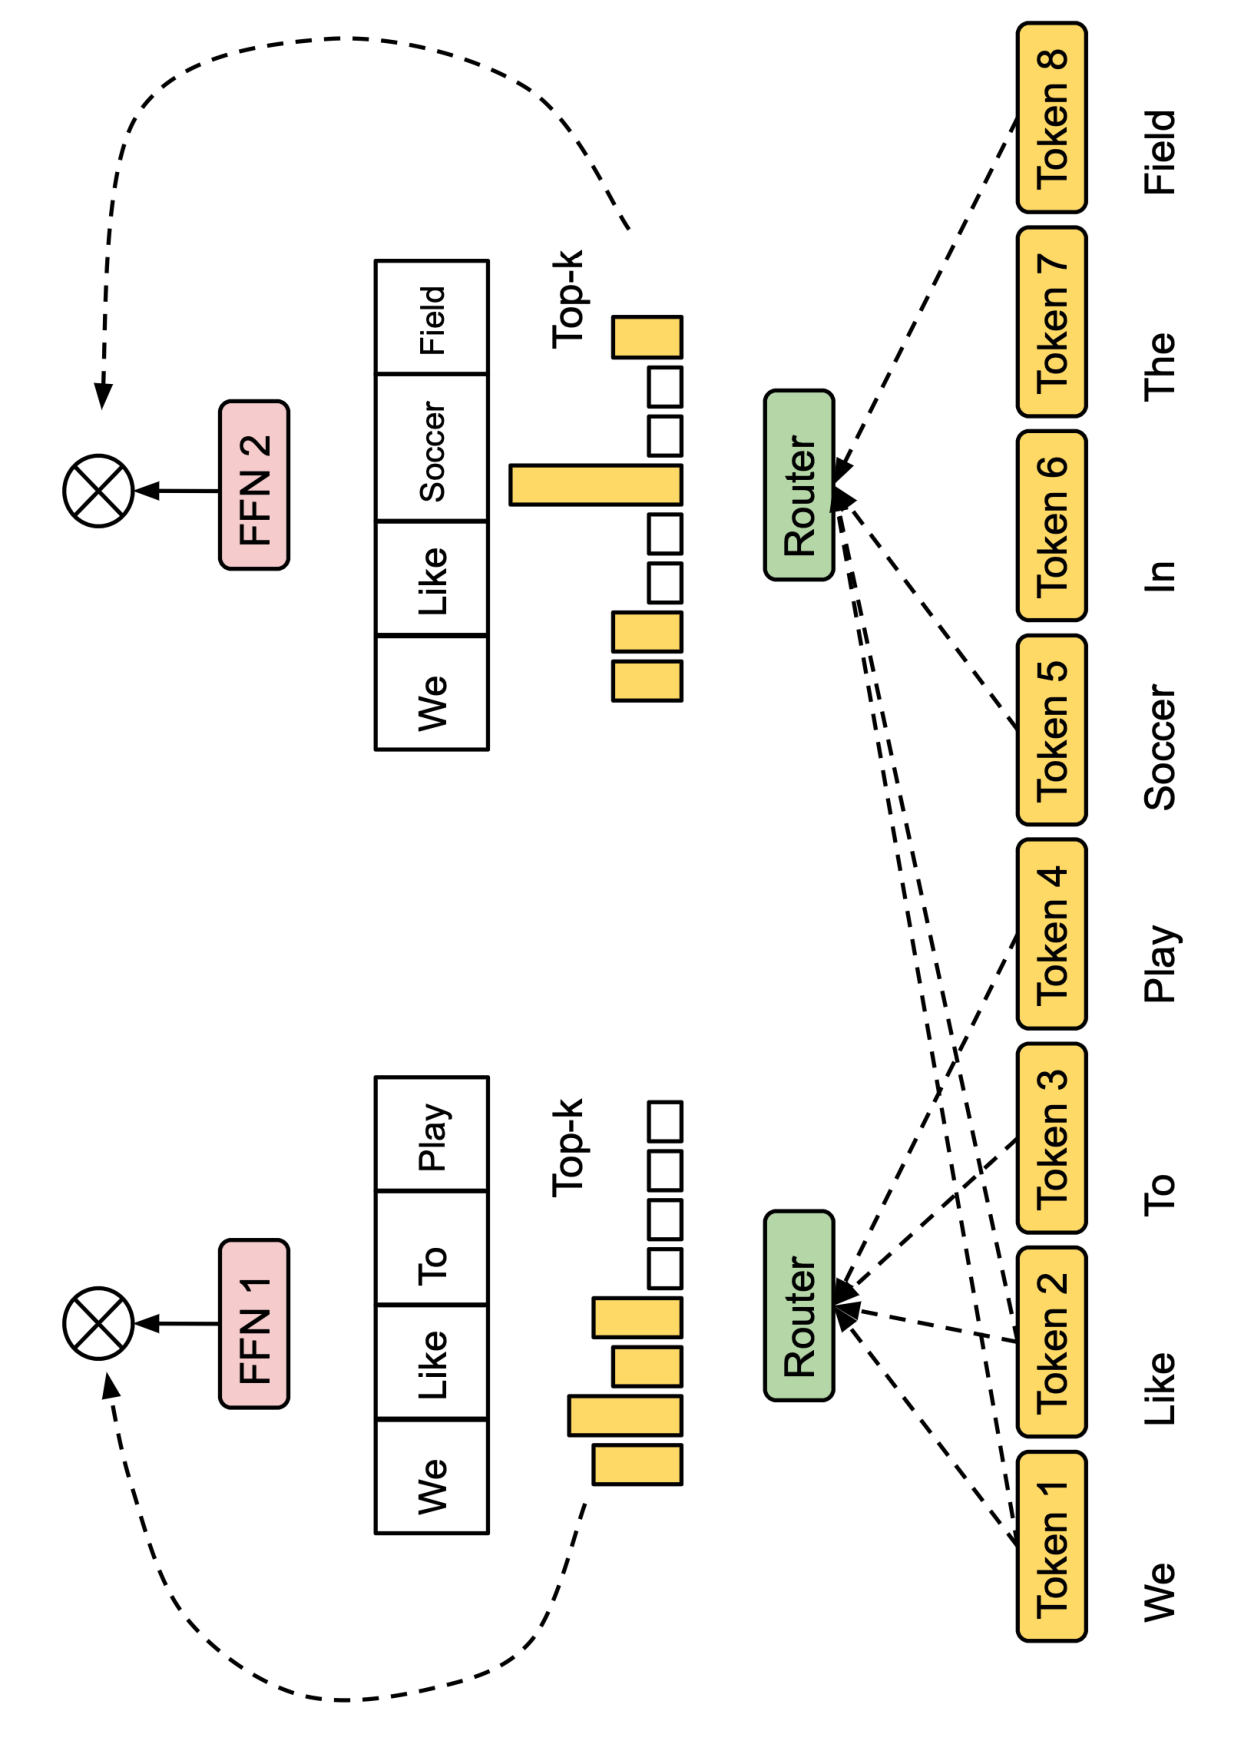
\includegraphics[angle=-90,width=0.9\linewidth]{figures/expert-to-token.pdf}
    \caption{“专家选择词元”的策略\cite{Zhou2022MixtureofExpertsWE}}
    \label{fig:expert-to-tokem}
\end{figure}


具体的路由过程如下：
\begin{enumerate}
    \item \textbf{计算亲和度分数：} 与经典路由类似，首先计算每个词元与每个专家之间的亲和度分数。对于输入词元表征矩阵$X \in \mathbb{R}^{n \times d}$和专家嵌入矩阵$W_g \in \mathbb{R}^{d \times E}$，亲和度分数矩阵$S \in \mathbb{R}^{n \times E}$通过softmax函数计算得出：
    \begin{equation}
        S = \text{softmax}(X \cdot W_g)
    \end{equation}
    \item \textbf{专家选择词元：} 对分数矩阵$S$的转置$S^T$进行操作，每个专家（$S^T$的每一行）从中选择分数最高的$k$个词元。这一步确定了每个专家处理的词元集合。
    \item \textbf{计算与输出：} 被选中的词元被送入对应的专家网络进行计算。由于一个词元可能被多个专家选中，它会从多个专家那里获得输出。最终的输出是所有处理过该词元的专家输出的加权和。
\end{enumerate}
通过这种方式，每个专家的计算负载是完全相同的（都处理$k$个词元），从而无需额外的负载均衡损失。同时，一个词元被处理的次数（即激活的专家数）是可变的，这取决于它被多少专家选为“Top-k”亲和度的词元，从而实现了对不同词元的计算资源的动态分配。但是，由于分配时需要知道整句句子的信息，这类方法对编码器模型较为友好，对解码器模型应用起来则较为困难。


\subsection{基于输入难度的动态路由}
与专家选择路由不同，另一类方法保留了“词元选择专家”的框架，但将激活的专家数量$k$从一个固定的超参数变为一个根据输入动态决定的变量。其核心假设是“更难的任务需要更多的专家”。Huang等人提出的动态路由机制\cite{Huang2024HarderTN}（图\ref{fig:top-p-routing}）是其中的一个代表。

\begin{figure}[h]
    \centering
    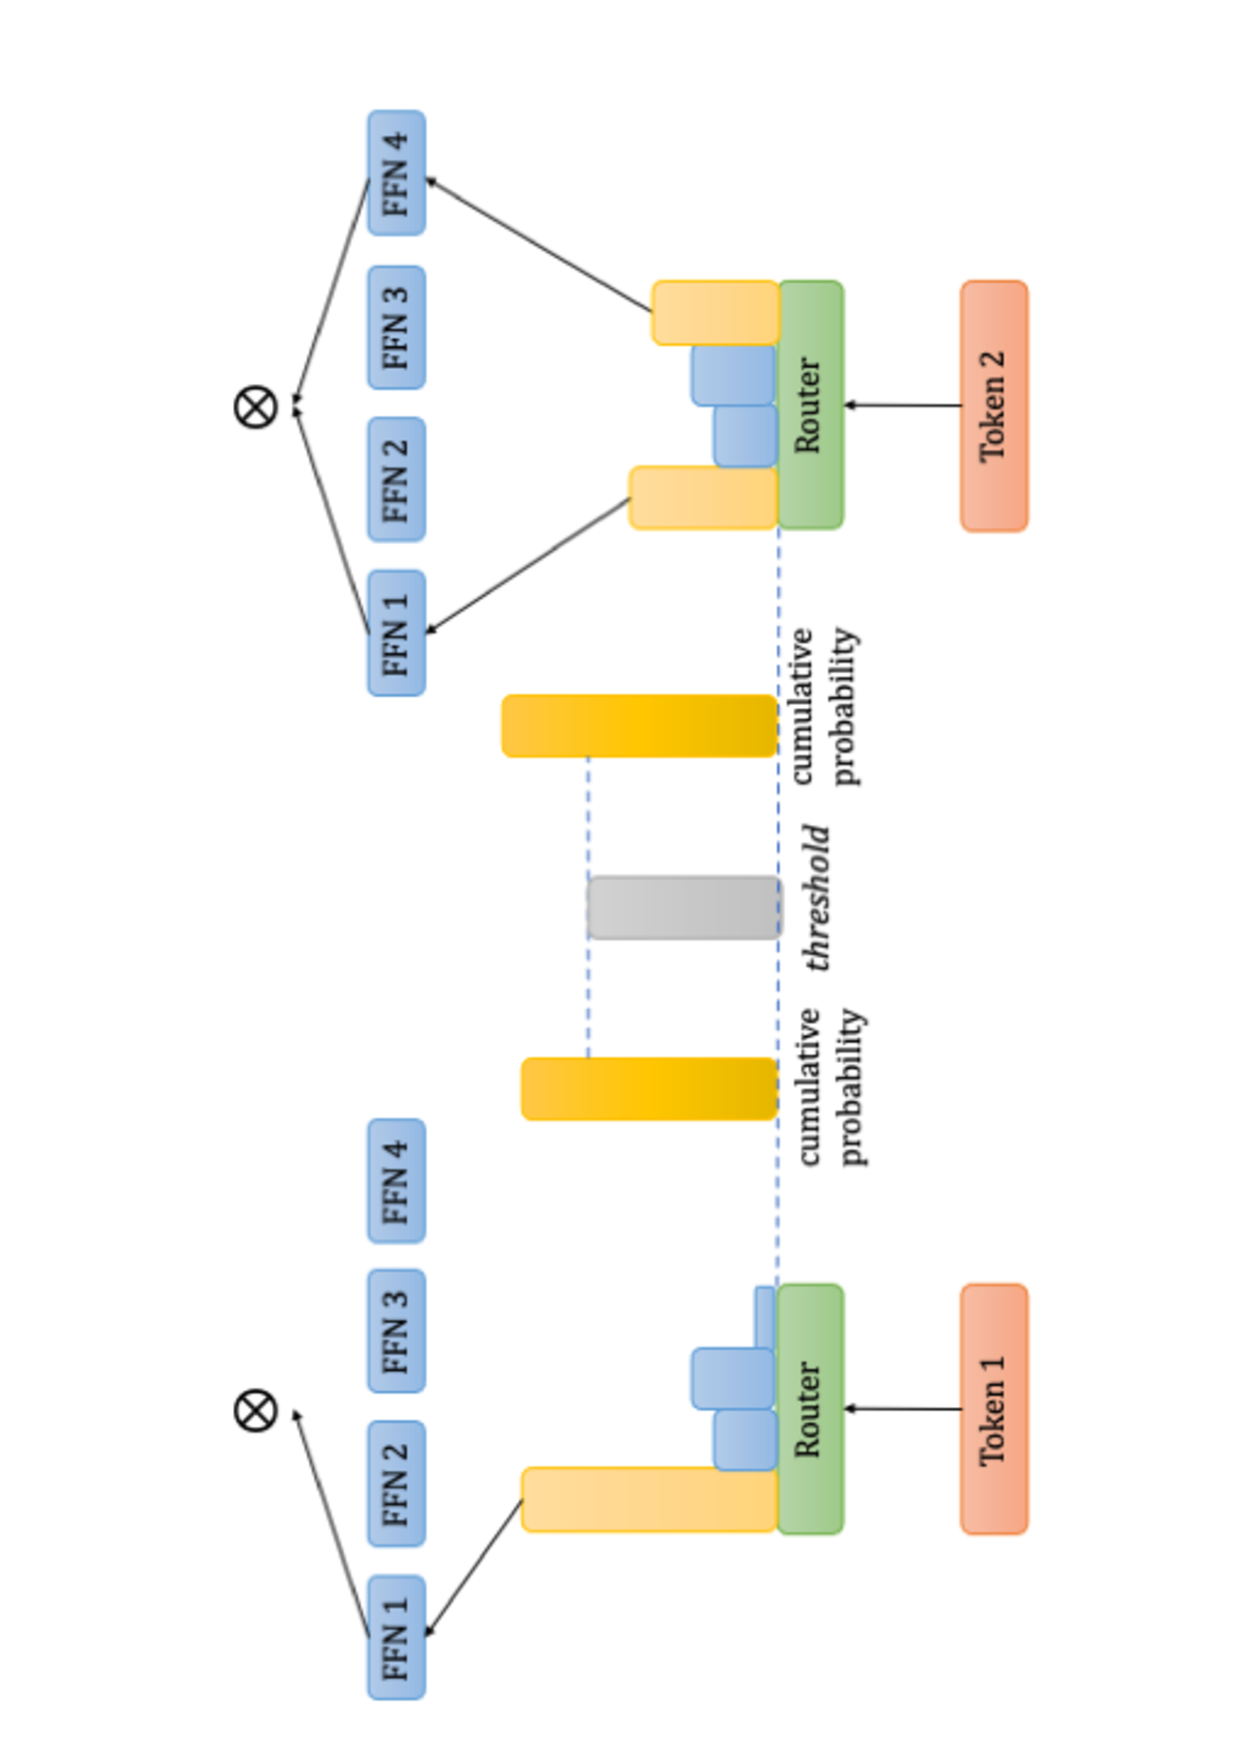
\includegraphics[angle=-90,width=0.9\linewidth]{figures/top-p-routing.pdf}
    \caption{基于置信度的专家选择策略\cite{Huang2024HarderTN}}
    \label{fig:top-p-routing}
\end{figure}

该方法引入了一种基于置信度的专家选择策略，其工作流程如下：
\begin{enumerate}
    \item \textbf{计算专家概率：} 对于一个输入词元，路由器首先计算出一个概率分布$P$，表示该词元分配给各个专家的概率。
    \item \textbf{动态专家选择：} 将专家按照概率从高到低排序。然后，模型会累加这些概率，直到累积概率超过一个预设的阈值$p$（例如0.9）。被累加的这些专家就是最终被激活的专家。激活的专家数量$t$由下式决定：
    \begin{equation}
        t = \arg\min_k \left( \sum_{i=1}^{k} P_i \geq p \right)
    \end{equation}
    其中$P_i$是排序后第$i$个专家的概率。这种策略也被称为Top-P路由。
    \item \textbf{动态损失函数：} 为了防止模型通过降低所有专家的概率来“作弊”并激活大量专家，该方法引入了一个动态损失函数$L_d$来鼓励路由器产生更稀疏（即更集中）的概率分布。这个损失函数实际上是概率分布$P$的熵：
    \begin{equation}
        L_d = \sum_{i=1}^{E} -P_i \log(P_i)
    \end{equation}
    通过最小化这个熵损失，模型被激励将概率集中在少数几个专家上，从而在没有明确限制的情况下也能实现稀疏激活。
\end{enumerate}
这种机制使得模型能够为它认为“简单”的词元（即路由器给出一两个高置信度专家）分配较少的专家，而为“复杂”的词元（即路由器给出的专家概率分布较为平坦）分配更多的专家，实现了更精细化的计算资源分配。

\subsection{动态混合专家模型 (DynMoE)}
Guo等人提出的动态混合专家模型（Dynamic Mixture of Experts, DynMoE）\cite{Guo2024DynamicMO}则是一种更为彻底的自适应方法，它不仅能自动决定每个词元激活的专家数量，还能在训练过程中动态地调整专家总数（图\ref{fig:dynmoe}）。

\begin{figure}[h]
    \centering
    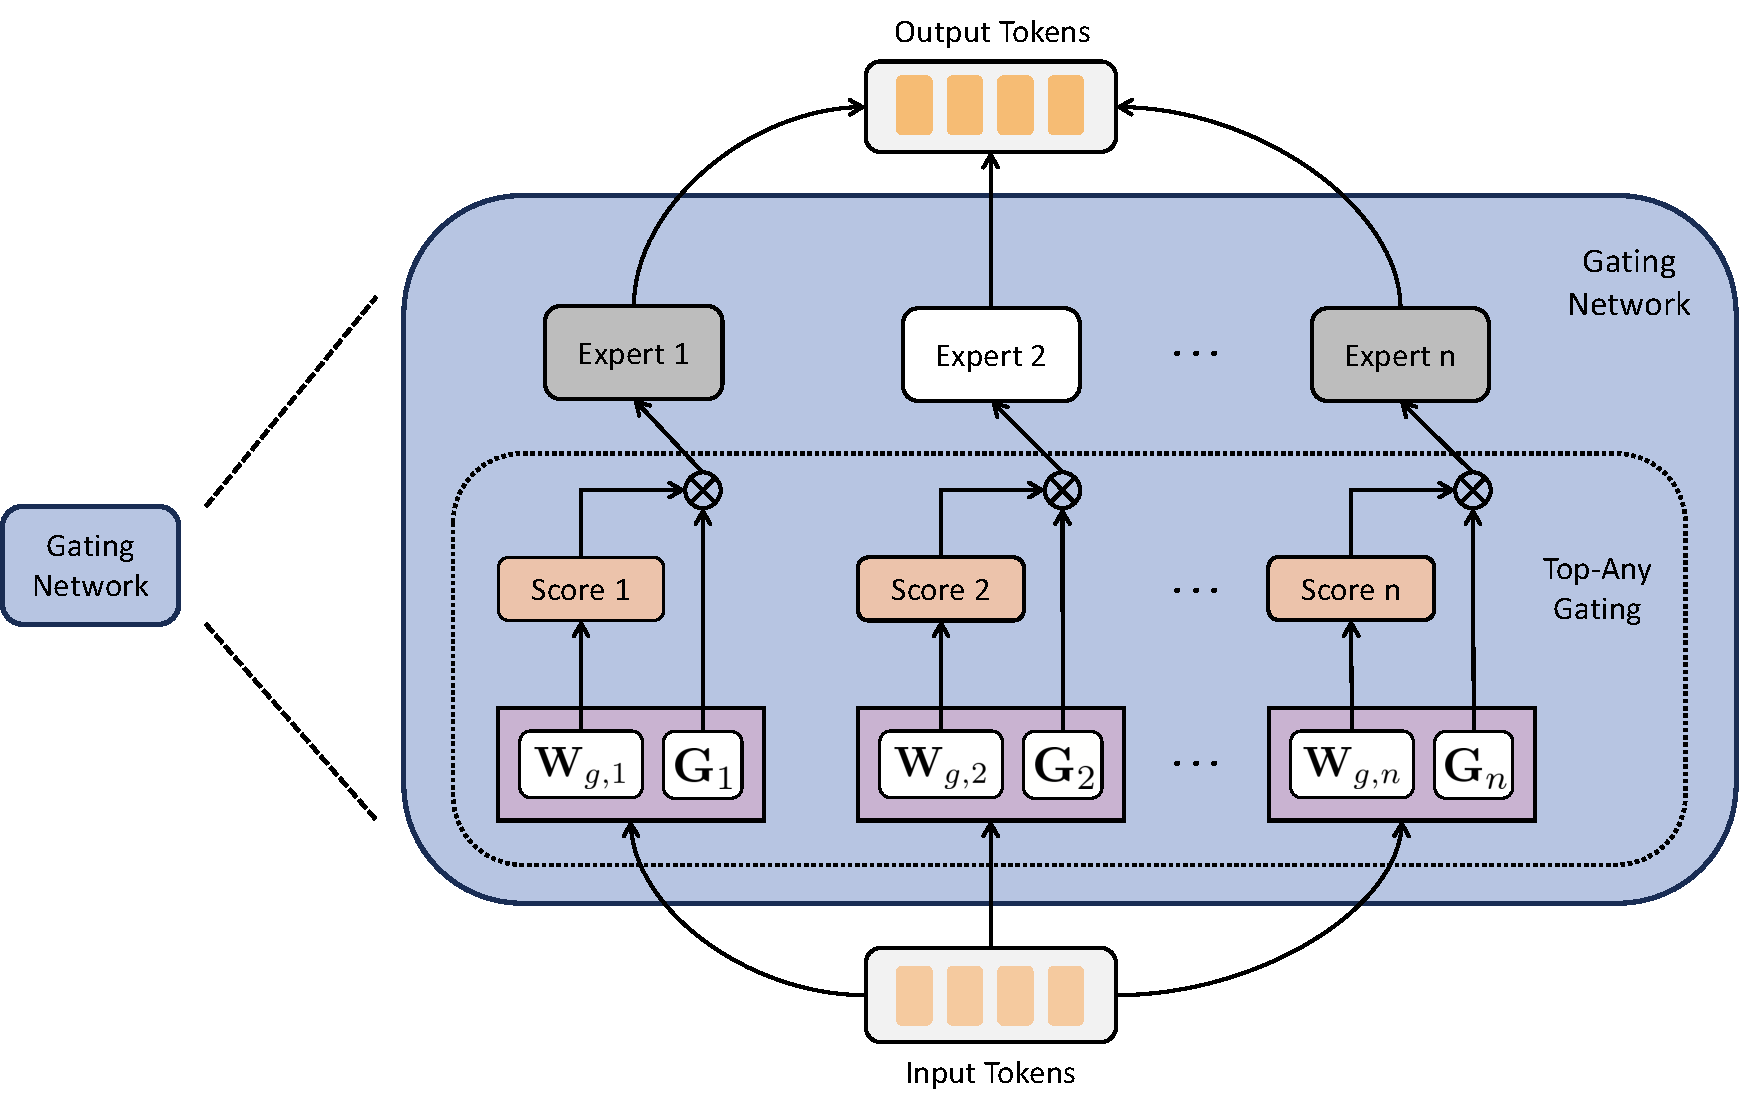
\includegraphics[width=0.85\linewidth]{figures/dynmoe.pdf}
    \caption{DynMoE架构\cite{Guo2024DynamicMO}}
    \label{fig:dynmoe}
\end{figure}

DynMoE的核心创新包括：
\begin{enumerate}
    \item \textbf{Top-any门控机制：} 该机制将专家选择问题建模为一个多标签分类问题。每个专家都被视为一个独立的类别。对于输入词元$x$和专家嵌入$W_g$，模型首先计算它们之间的余弦相似度分数$s(x)$。然后，每个专家$e$都有一个可学习的激活阈值$G_e$。如果词元$x$与专家$e$的相似度分数经过sigmoid函数变换后大于该专家的阈值，则该专家被激活：
    \begin{equation}
        g(x)_e = 
        \begin{cases}
            1 & \text{if } \sigma(s(x)_e) > \sigma(G_e) \\
            0 & \text{otherwise}
        \end{cases}
    \end{equation}
    这种机制允许一个词元激活任意数量的专家，包括零个。为了防止在推理过程中丢弃词元，对于没有激活任何专家的词元，系统会退回到Top-1路由策略。

    \item \textbf{专家数量自适应调整：} 在训练过程中，DynMoE会监控专家的使用情况，并动态地增加或删减专家。
    \begin{itemize}
        \item \textbf{增加专家：} 如果在一个训练批次中，存在一些词元没有激活任何专家，模型会根据这些词元的平均嵌入向量来初始化一个新的专家。
        \item \textbf{移除专家：} 如果一个专家在连续的很多训练步骤中都未被任何词元激活，它就会被视作冗余专家并被移除。
    \end{itemize}
    \item \textbf{新的辅助损失函数：} 为了在这种灵活的路由机制下保证稀疏性，DynMoE引入了一个“稀疏且简单的门控损失”（sparse and simple gating loss）。该损失由两部分组成：
    \begin{itemize}
        \item \textbf{多样性损失（Diversity Loss）：} $L_{div} = ||W_g^T W_g - I||_F^2$。该损失鼓励不同专家的嵌入向量相互正交，从而使它们学习到更多样化的特征。
        \item \textbf{简洁性损失（Simplicity Loss）：} $L_{sim} = \sum_e ||w_{g,e}||_2$。该损失对专家嵌入向量的L2范数进行惩罚，以维持数值稳定性。
    \end{itemize}
\end{enumerate}
DynMoE通过上述机制，实现了对MoE模型超参数（激活专家数$k$和专家总数$E$）的自动调整，极大地减少了模型设计和调优所需的人工和计算成本。

\section{前馈网络之外的混合专家模型}
\label{sec:moe_beyond_ffn}
经典的混合专家模型主要将专家网络应用于Transformer中的前馈网络 (FFN) 部分。然而，条件计算 (Conditional Computation) 的思想具有更广泛的适用性。学术界已经开始探索将混合专家机制与其他模块相结合，甚至重塑整个模型架构的计算流程，旨在将模型的动态性和稀疏性提升到新的水平。本节将介绍若干代表性的前沿工作，它们将混合专家模型的思想从前馈网络扩展到了注意力机制、整体模块组合乃至记忆等多个维度。

\subsection{混合注意力头（MoA）}
混合注意力头 (Mixture of Attention Heads, MoA) \cite{Zhang2022MixtureOA} 将混合专家模型的理念直接应用于多头注意力机制 (Multi-Head Attention, MHA) 中，而非传统的前馈网络层（图\ref{fig:moa}）。其核心思想是，并非每个输入词元都需要所有注意力头的参与，而是可以根据上下文动态地选择一个最相关的子集。

\begin{figure}[h]
    \centering
    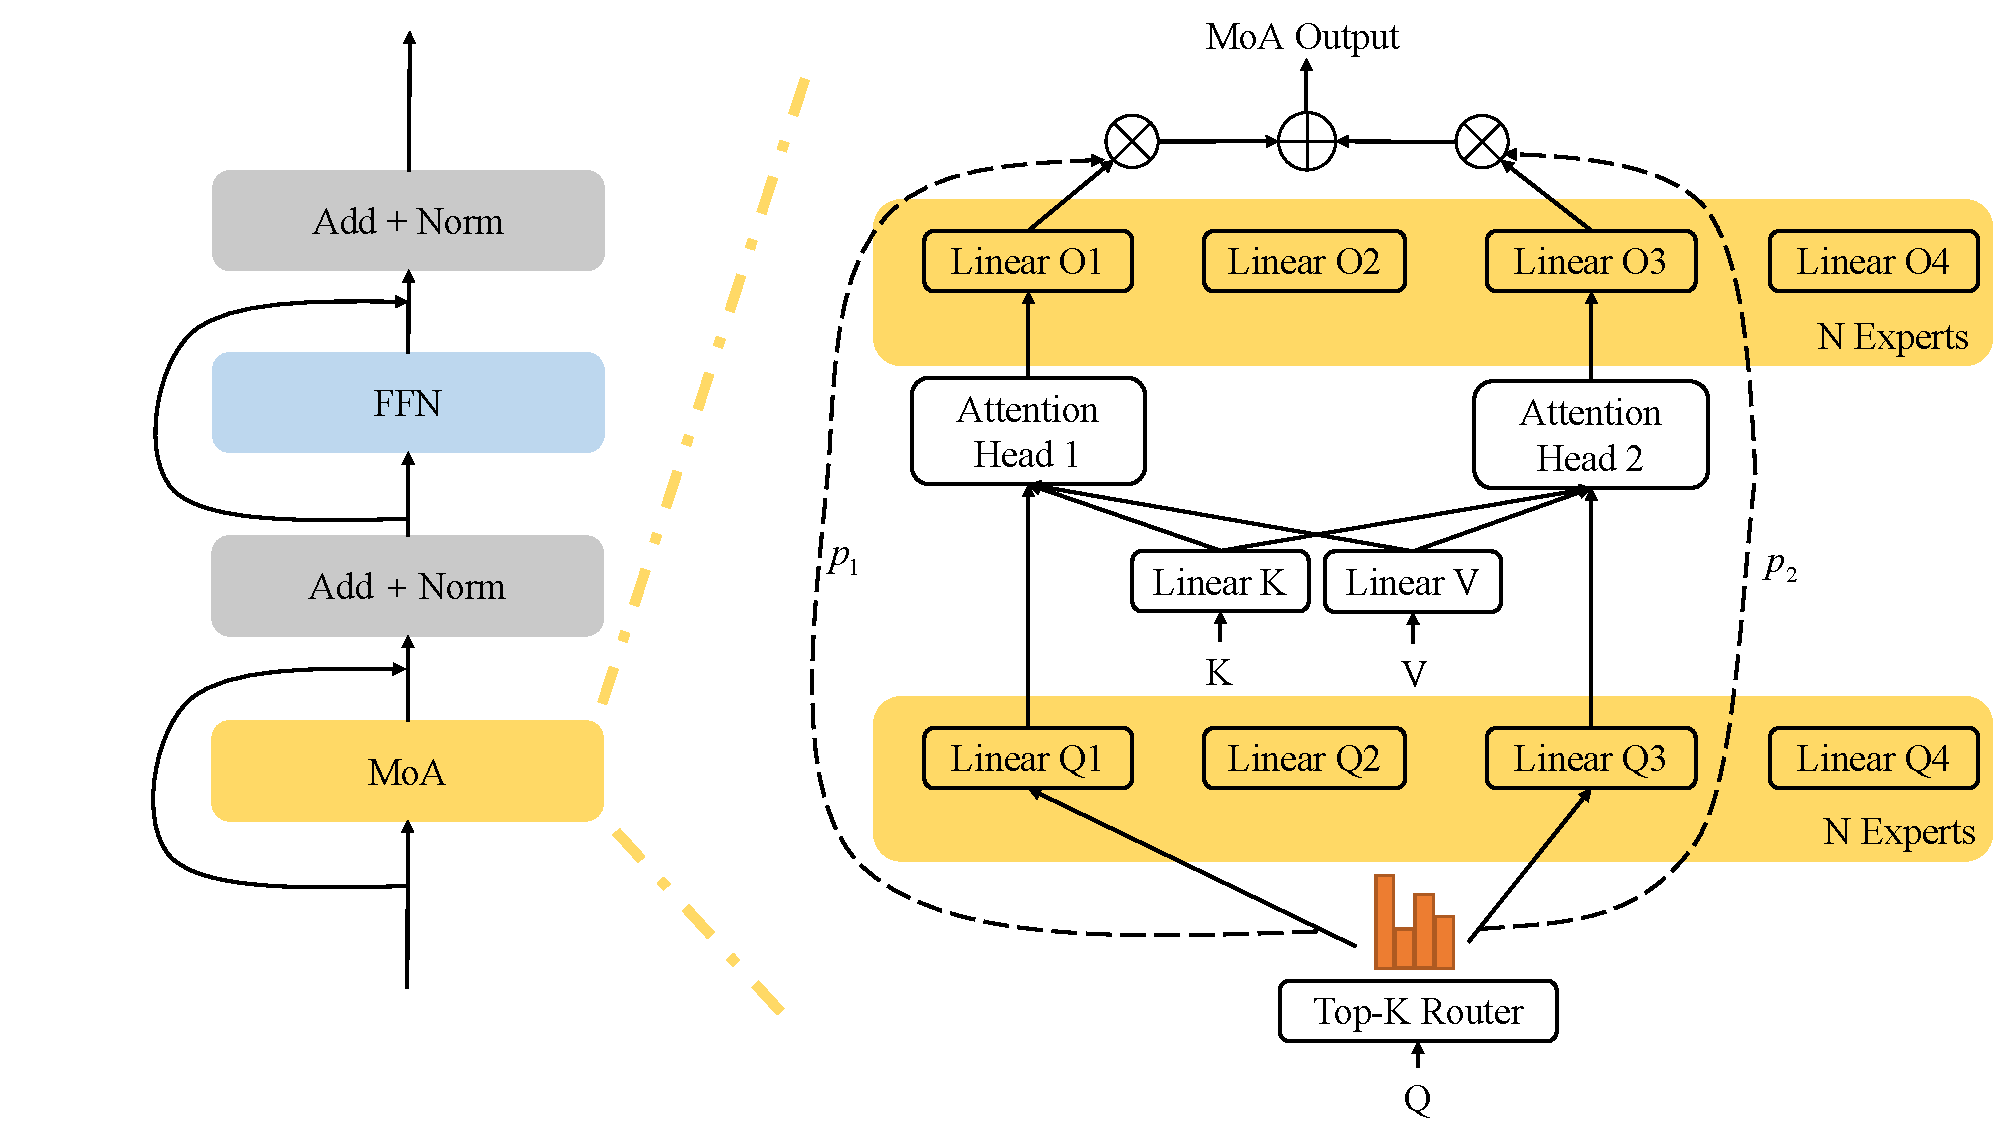
\includegraphics[width=0.9\linewidth]{figures/MoA.pdf}
    \caption{混合注意力头架构\cite{Zhang2022MixtureOA}}
    \label{fig:moa}
\end{figure}

在MoA架构中，存在一个包含$N$个“注意力专家” (Attention Experts) 的专家池，其中每个专家本质上就是一个拥有独立参数的注意力头。对于输入序列中的每一个词元$x$，一个可学习的路由器 (Router) 会计算该词元与所有$N$个注意力专家的亲和度得分，并从中选择得分最高的$k$个专家来处理该词元。最终的注意力输出是这$k$个被激活专家输出的加权和，其权重由路由器的得分归一化后得到。

为了在扩大专家数量的同时控制计算和参数开销，MoA采用了一种高效的设计: 它在所有注意力专家之间共享键 (Key, $W^K$) 和值 (Value, $W^V$) 的投影矩阵，仅保留查询 (Query, $W^Q$) 和输出 (Output, $W^O$) 的投影矩阵为每个专家私有。这样，计算代价高昂的$K, V$矩阵变换只需执行一次，而每个专家只需进行轻量级的$Q$向量投影和输出计算。

与标准混合专家模型类似，MoA也引入了辅助损失函数$L_{\text{aux}}$来促进专家间的负载均衡，防止少数专家被过度使用。其形式如下:
\begin{equation}
    L_{\text{aux}}(Q) = N \cdot \sum_{i=1}^{N} f_i \cdot P_i
\end{equation}
其中，$Q$代表一个批次中的所有词元查询，$N$是专家总数，$f_i$是第$i$个专家被分配到的词元数量占比，$P_i$是第$i$个专家在整个批次中获得的路由门控概率之和。该损失函数旨在平衡每个专家的使用频率和门控权重，鼓励模型更均匀地利用所有专家。实验证明，MoA能够在提升模型性能的同时，保持计算效率，并为模型可解释性提供了新的视角，因为不同的注意力专家倾向于学习不同的语言功能\cite{Zhang2022MixtureOA}。

\subsection{混合深度（MoD）}
混合深度 (Mixture-of-Depths, MoD)\cite{Raposo2024MixtureofDepthsDA} 是一种旨在动态分配计算资源的架构，它允许不同的词元在模型中经历不同数量的计算层，即拥有不同的计算“深度”。与传统的混合专家模型在宽度上扩展 (选择不同的专家) 不同，MoD在深度上进行稀疏化 (选择是否执行计算)（图\ref{fig:mod}）。

\begin{figure}[h]
    \centering
    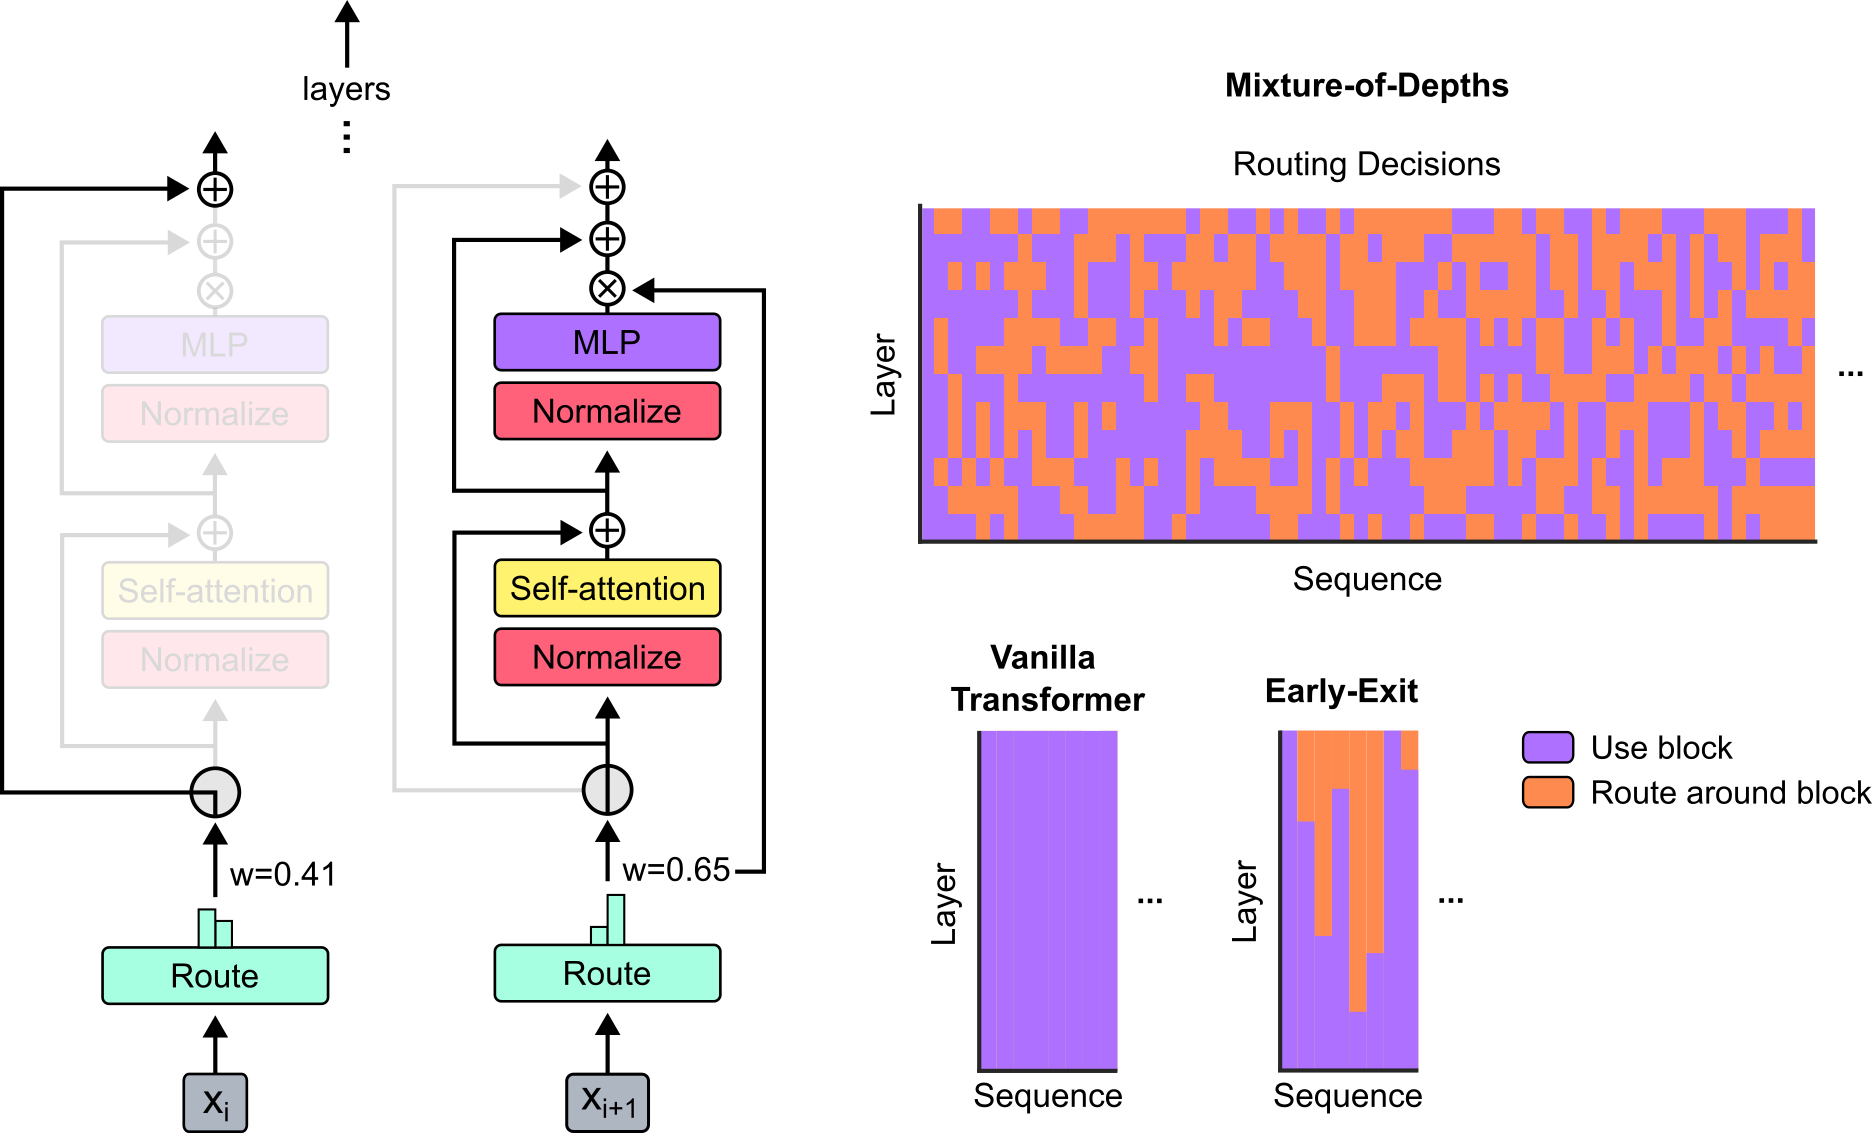
\includegraphics[width=1.0\linewidth]{figures/mod.png}
    \caption{混合深度架构\cite{Raposo2024MixtureofDepthsDA}}
    \label{fig:mod}
\end{figure}

其核心机制是，在Transformer的每个块 (Block) 前都设置一个路由器。对于输入序列中的每个词元，路由器会决定该词元是进入该块进行标准的自注意力和前馈网络计算，还是直接通过残差连接“跳过”该块。为了维持固定的计算预算并与现代硬件兼容，MoD采用了“专家选择” (Expert Choice)\cite{Zhou2022MixtureofExpertsWE} 的路由策略。在此策略中，并非由词元选择路径，而是由每个计算块 (被视为“专家”) 从所有输入词元中选择亲和度最高的$k$个词元进行处理。其余的$S-k$个词元则被跳过。

这种方式确保了每个块处理的词元数量是恒定的$k$，从而使计算图保持静态，极大地提升了训练和推理的效率。模型的计算开销仅与容量因子$k/S$成正比，而与序列长度无关。一个词元的最终计算路径由其在各层被路由决策的序列决定，例如一个词元可能跳过浅层块，但在深层块中被处理。

由于“专家选择”在训练时需要获取整个序列的信息来确定top-k，这在自回归生成任务的推理阶段是不可行的 (因为未来的词元尚不存在)。为了解决这个问题，MoD提出训练一个辅助的预测性路由器 (predictive router)，该路由器仅基于当前词元的信息来预测其是否会被主路由器选中，从而在推理时实现因果一致的动态路由\cite{Raposo2024MixtureofDepthsDA}。

\subsection{混合模块（MoM）}
混合模块（Mixture-of-Modules, MoM）\cite{Gong2024MixtureofModulesRT} 是一种颠覆性的架构，它彻底打破了传统Transformer模型固定的、自下而上的分层计算模式。其核心思想是将整个Transformer重塑为一个由基础模块 (Modules) 构成的集合，并通过动态路由来为每个词元“组装”出一个独特的计算图（图\ref{fig:mixtureofmodules}）。

\begin{figure}[h]
    \centering
    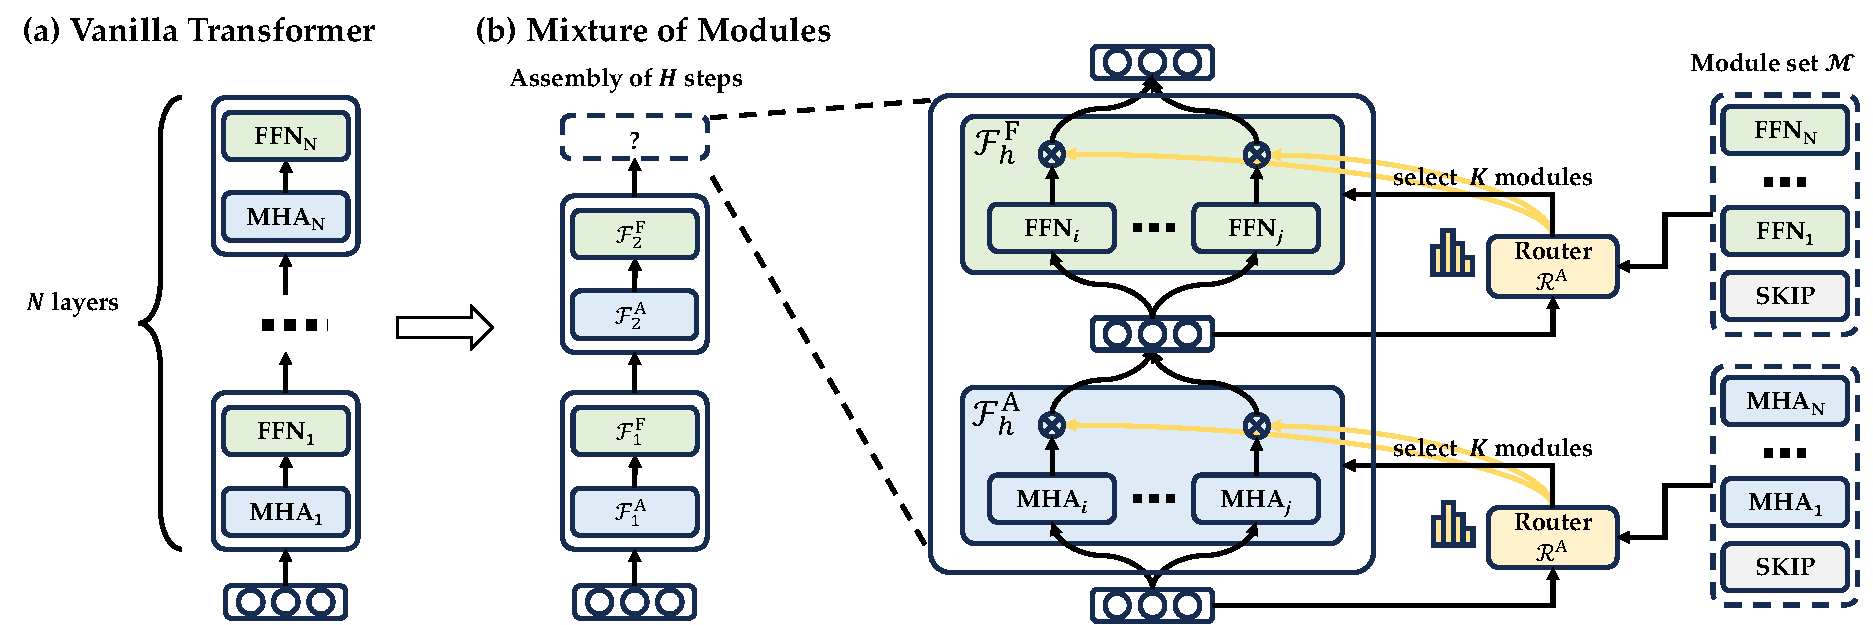
\includegraphics[width=1.0\linewidth]{figures/mixtureofmodules.pdf}
    \caption{混合模块架构\cite{Gong2024MixtureofModulesRT}}
    \label{fig:mixtureofmodules}
\end{figure}

MoM架构包含一个由多个独立的多头注意力机制模块和前馈网络模块组成的“模块池”。在处理每个词元时，计算过程不再是依次通过固定的第1层、第2层……，而是分为多个迭代步骤。在每个步骤中，模型通过两个独立的路由器——一个用于多头注意力机制模块，另一个用于前馈网络模块——从模块池中各自选择$K$个最合适的模块。这些被选中的模块的输出通过路由权重进行加权求和，形成该步骤的最终输出，并作为下一步的输入。整个前向传播过程就是这样一个动态构建和执行计算路径的过程。

与依赖于前一层输出的传统模型不同，MoM的路由器在做决策时需要感知历史选择信息。为此，MoM的路由器内部集成了一个门控循环单元（Gated Recurrent Unit, GRU）\cite{Cho2014LearningPR}，其隐藏状态$s_h^X$在每个组装步骤$h$中进行更新:
\begin{equation}
    s_h^X = \text{GRU}^X(x_h, s_{h-1}^X), \quad X \in \{\text{MHA}, \text{FFN}\}
\end{equation}
其中$x_h$是当前步骤的输入，$s_{h-1}^X$是上一状态。路由权重$r_h^X$则由当前状态$s_h^X$通过一个线性变换得到:
\begin{equation}
    r_h^X = W^X s_h^X
\end{equation}
这种设计允许路由决策具有记忆性，从而能够构建出更加复杂和协调的计算路径。

MoM不仅为Transformer的过参数化问题提供了新的解决方案，还统一了层跳过 (Layer-skipping)\cite{Teerapittayanon2016BranchyNetFI,Xin2021BERxiTEE,Elhoushi2024LayerSkipEE}、参数共享\cite{Dehghani2018UniversalT,Lan2019ALBERTAL}和混合专家等多种动态计算机制的框架\cite{Gong2024MixtureofModulesRT}。

\subsection{混合递归 (MoR)}
混合递归（Mixture-of-Recursions, MoR）\cite{Bae2025MixtureofRecursionsLD} 是一个统一了参数共享和自适应计算两大效率提升范式的框架（图\ref{fig:mor_overview}）。它基于循环Transformer（Recursive Transformer）\cite{Bae2024RelaxedRT,Fan2024LoopedTF,Giannou2023LoopedTA,Yang2023LoopedTA,Saunshi2025ReasoningWL} 的思想，即在多个计算步骤中重复使用同一组共享的层（一个“递归块”），但其创新之处在于，每个词元所经历的递归“深度” （即重复次数） 是动态可学习的。

\begin{figure}[h]
    \vspace{-7pt}
    \centering
    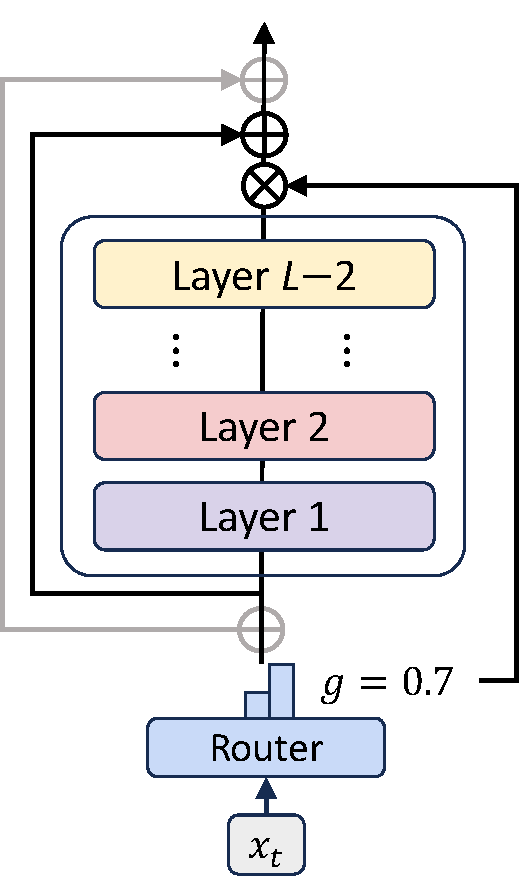
\includegraphics[width=0.23\columnwidth]{figures/overview/overview_main1.pdf}
    \hspace{23pt}
    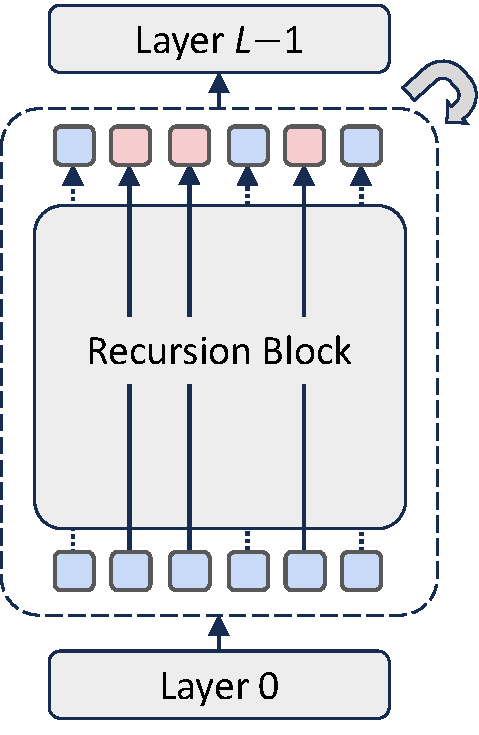
\includegraphics[width=0.238\columnwidth]{figures/overview/overview_main2.pdf}
    \hspace{7pt}
    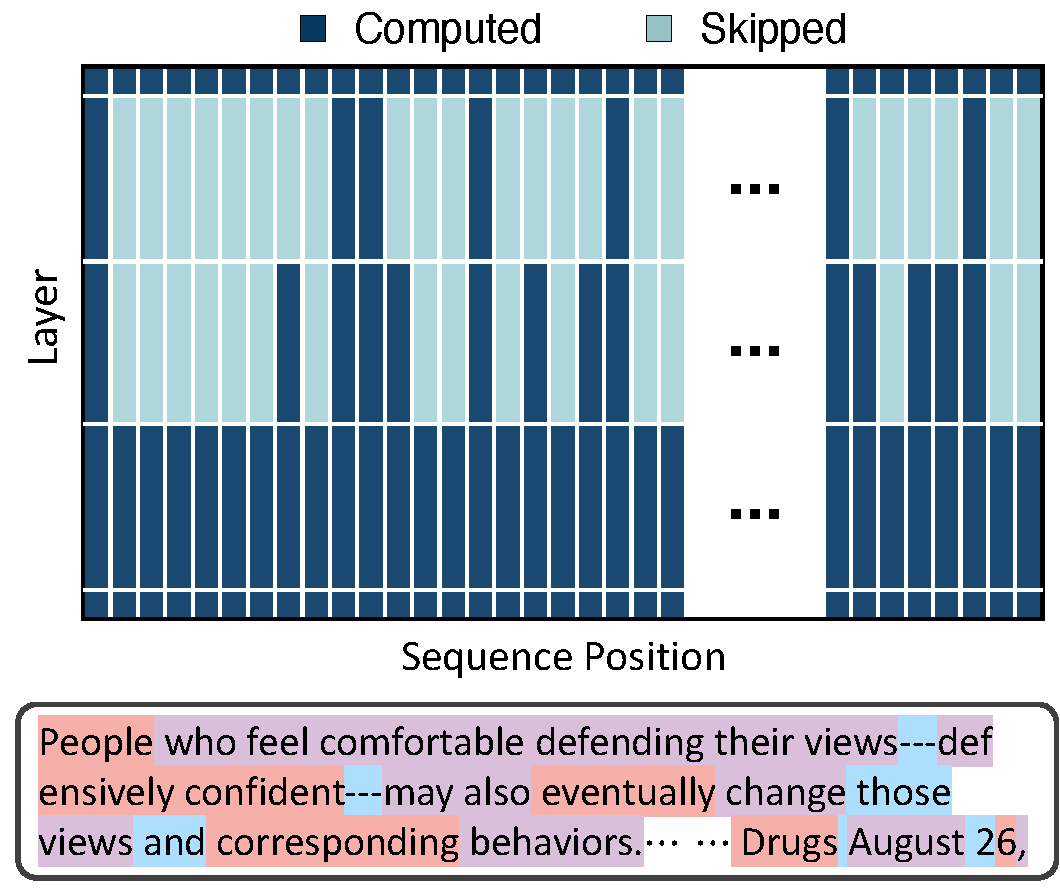
\includegraphics[width=0.42\columnwidth]{figures/overview/overview_main3.pdf}
    \caption{MOR的示意图\cite{Bae2025MixtureofRecursionsLD}}
    \label{fig:mor_overview}
\end{figure}

MoR的核心是一个轻量级路由器，它为输入序列中的每个词元$x_t$分配一个特定的递归次数$N_t$。这意味着，模型可以为它认为“困难”的词元分配更多的计算步骤（更大的$N_t$），而为“简单”的词元分配更少的计算步骤，从而实现细粒度的、自适应的计算资源分配。这种机制被类比为模型的“思考深度”。

该架构不仅通过参数共享大幅减少了模型的参数量，还通过动态路由显著降低了前向传播所需的总计算量 (FLOPs)。此外，MoR为动态深度模型设计了专门的键值缓存（KV Caching）策略:
\begin{itemize}
    \item \textbf{递归维度缓存（Recursion-wise Caching）}: 每个递归深度层级都拥有自己独立的KV缓存。只有在特定深度被激活的词元，其键值对才会被缓存并用于该层的注意力计算。
    \item \textbf{递归KV共享（Recursive KV Sharing）}: 所有词元在第一个递归步骤中产生的键值对被缓存，并在后续所有递归步骤中共享使用。
\end{itemize}
这些策略进一步优化了推理过程中的内存占用和访存效率。实验表明，MoR在同等训练FLOPs和更小模型尺寸下，能够达到乃至超越标准Transformer和固定深度循环模型的性能，形成了一个新的帕累托前沿\cite{Bae2025MixtureofRecursionsLD}。

\subsection{混合记忆（Mixture-of-Memories）}
混合记忆（Mixture-of-Memories, MoM）（图\ref{fig:mixtureofmemories}）\cite{Du2025MoMLS} 将混合专家的思想应用于线性序列模型（如线性注意力、状态空间模型等）的核心瓶颈——其固定大小的记忆状态（memory state）。传统线性模型将整个历史信息压缩到一个单一的记忆状态中，容易导致“记忆干扰”（memory interference）和容量受限，在需要精确回忆长距离信息的任务上表现不佳。

\begin{figure}[h]
    \centering
    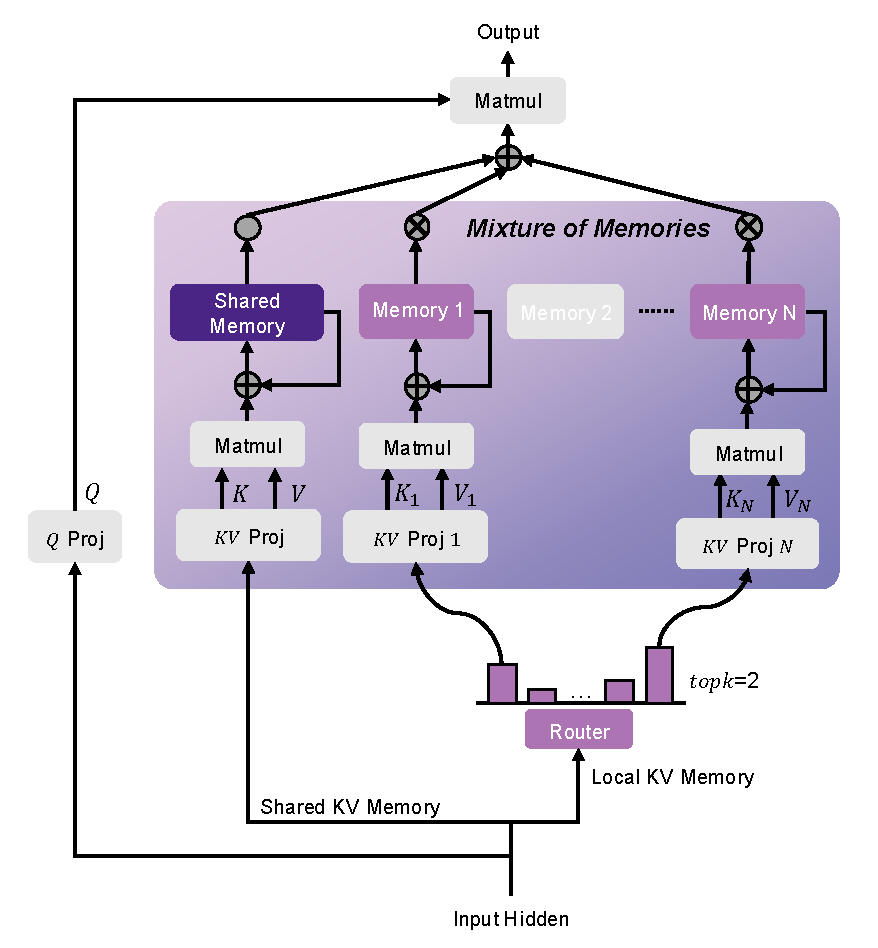
\includegraphics[width=0.8\linewidth]{figures/mom_fig1.pdf}
    \caption{混合记忆架构\cite{Du2025MoMLS}}
    \label{fig:mixtureofmemories}
\end{figure}

MoM架构的创新之处在于引入了多个独立的记忆状态，称之为“记忆专家”（Memory Experts）。其工作流程如下:
\begin{enumerate}
    \item \textbf{路由}: 对于每个输入词元$x_t$，一个路由器会计算其与所有$M$个记忆专家的相关性得分，并选择top-k个最相关的记忆进行更新。
    \item \textbf{并行更新}: 输入词元$x_t$被投影为$k$组独立的键值对 $(k_t^m, v_t^m)$，分别用于更新被选中的$k$个记忆状态$M_{t-1}^m$:
    \begin{equation}
        M_t^m = M_{t-1}^m + (k_t^m)^T v_t^m
    \end{equation}
    而未被选中的记忆状态则保持不变，$M_t^j = M_{t-1}^j$，从而避免了不相关信息的干扰。
    \item \textbf{记忆混合与查询}: 所有被激活的记忆状态根据路由器的门控权重$g_t^{(m)}$加权求和，形成一个临时的“混合记忆”$\bar{M_t}$:
    \begin{equation}
        \bar{M_t} = \sum_{m \in \text{TopK}(x_t)} g_t^{(m)} M_t^m
    \end{equation}
    最终的输出$o_t$由查询向量$q_t$与该混合记忆相互作用产生: $o_t = q_t \bar{M_t}$。
\end{enumerate}
通过将信息分流到不同的记忆通道，混合记忆极大地增强了模型的总记忆容量，并显著减轻了记忆干扰问题。这使得它在保持线性复杂度的同时，在各种依赖长程记忆的任务上性能大幅超越了其他线性模型，甚至能与标准的Transformer模型相媲美\cite{Du2025MoMLS}。

\section{专家选择的软性化}
经典的混合专家模型依赖于离散的路由决策，即为每个词元（token）选择或“硬性”分配特定的专家。这种离散性虽然实现了计算的稀疏化，但也使得路由器的训练变得困难，因为它本身不可微，必须依赖梯度直通估计（STE）等近似方法，这可能导致训练不稳定或收敛到次优解。为了解决这一问题，研究者们探索了将路由机制“软性化”的思路，通过引入可微的操作来替代离散的专家选择，从而实现端到端的稳定训练。

\subsection{Soft MoE}
Puigcerver等人提出的Soft MoE\cite{Puigcerver2023FromST} 是一种完全可微的稀疏Transformer变体。它与传统混合专家模型的核心区别在于，它执行的是隐式的“软性”分配，而非显式的“硬性”分配（图\ref{fig:SoftMoE}）。

\begin{figure}[h]
    \centering
    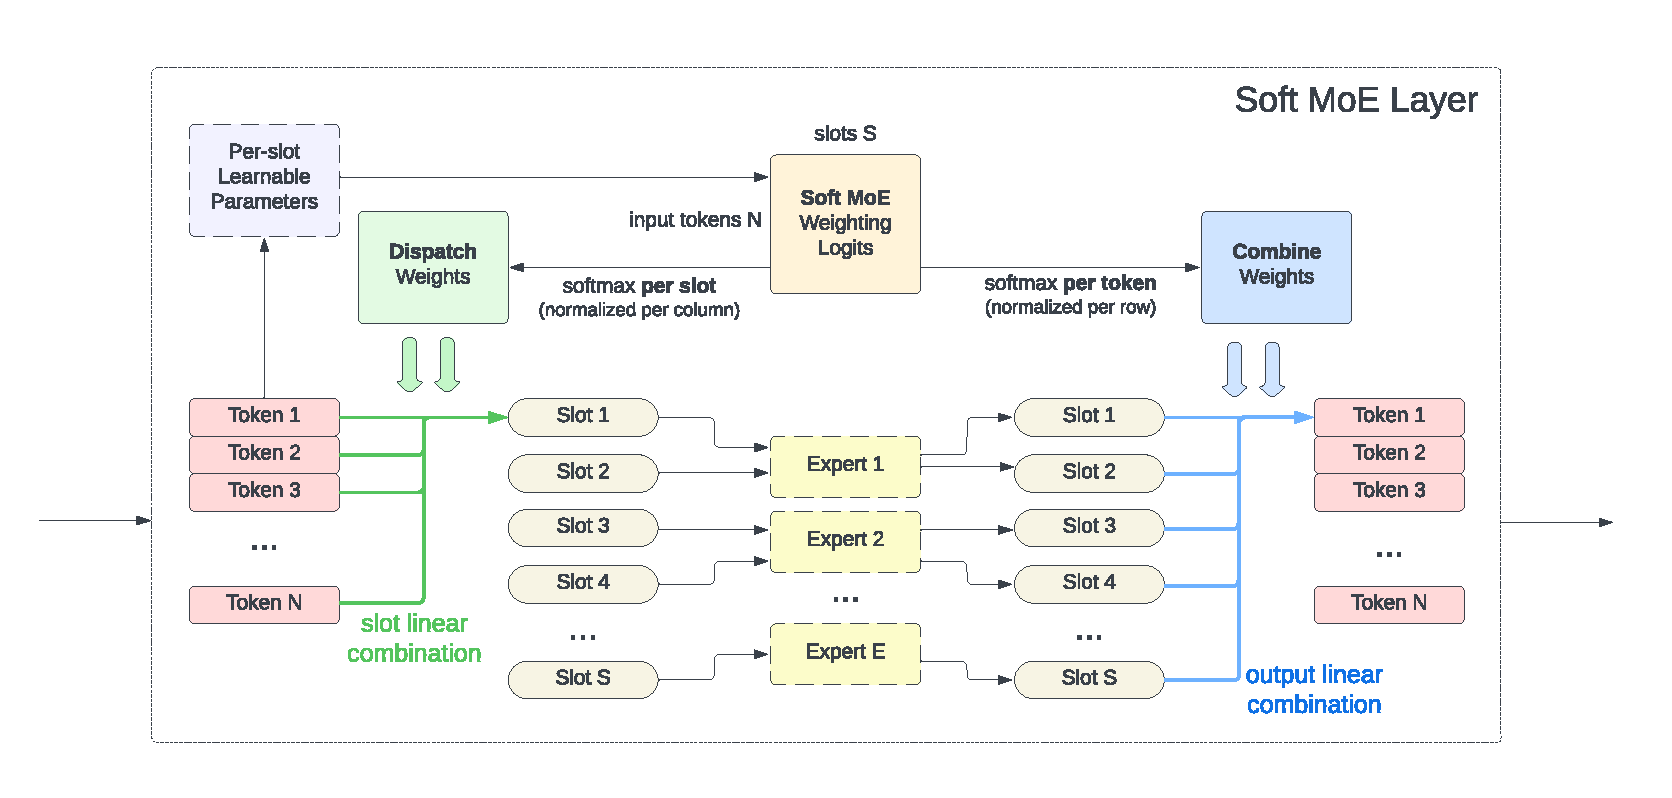
\includegraphics[width=1.0\linewidth]{figures/SoftMoE_diagram.pdf}
    \caption{Soft MoE的路由细节\cite{Puigcerver2023FromST}}
    \label{fig:SoftMoE}
\end{figure}

在经典的“词元选择专家”模式中，一个词元会被路由到少数几个专家。而在Soft MoE中，每个专家的输入不再是某个特定的词元，而是所有输入词元的加权平均。具体来说，假设一个序列的输入为 $X \in \mathbb{R}^{T \times d}$（$T$为序列长度，$d$为词元表征维度），专家数量为$N$，每个专家处理$p$个“槽位”（slot）。Soft MoE会为每个槽位（共$N \times p$个）生成一个输入表征$\tilde{x}$，该表征是所有$T$个输入词元的加权和。其槽位输入矩阵$\tilde{X} \in \mathbb{R}^{(N \cdot p) \times d}$ 的计算方式如下：
\begin{equation}
    \tilde{X} = D^T X
\end{equation}
其中，$D \in \mathbb{R}^{T \times (N \cdot p)}$ 是一个“分发权重”（Dispatch Weights）矩阵，通过对词元和槽位之间的亲和度得分进行softmax计算得到。这意味着每个槽位的输入都是对整个输入序列的一种“软性”关注。

在所有专家处理完各自的槽位输入后，模型的最终输出$Y$同样通过对所有专家槽位的输出$\tilde{Y}$进行加权求和得到：
\begin{equation}
    Y = C \tilde{Y}
\end{equation}
其中，$C \in \mathbb{R}^{T \times (N \cdot p)}$ 是“组合权重”（Combine Weights）矩阵，其计算方式与$D$类似。

通过这种方式，Soft MoE中的所有操作都是可微的，不再需要梯度估计。它避免了词元丢弃和负载不均衡问题，因为每个专家处理的计算量是固定的。实验表明，Soft MoE在保持混合专家模型优势的同时，训练过程更稳定，且性能优于传统的稀疏混合专家模型。

\subsection{SMEAR}
Muqeeth等人提出的SMEAR（Soft Merging of Experts with Adaptive Routing）\cite{Muqeeth2023SoftMO}提供了另一种实现路由软性化的思路。与Soft MoE混合（加权平均）词元输入不同，SMEAR的核心思想是混合专家的参数（图\ref{fig:smear}）。

\begin{figure}[h]
    \centering
    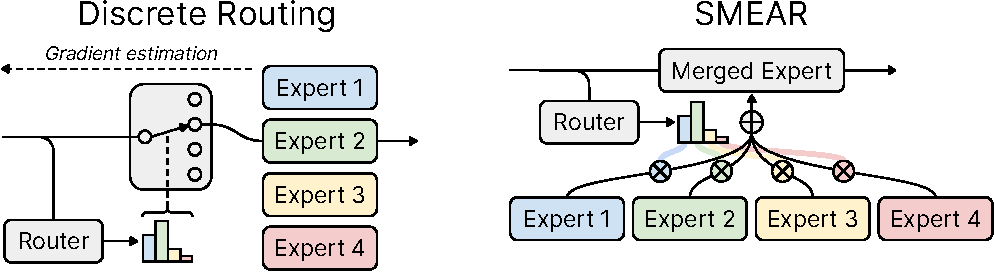
\includegraphics[width=1.0\linewidth]{figures/smear.pdf}
    \caption{SMEAR架构和普通混合专家模型的对比\cite{Muqeeth2023SoftMO}}
    \label{fig:smear}
\end{figure}

具体来说，对于一个输入$x$，路由器不再决定将$x$发送给哪个专家，而是计算出一组权重$G(x)$，用来对所有专家的参数进行加权平均，从而动态地构建出一个临时的“融合专家”（Merged Expert）。然后，输入$x$被这个融合专家处理，得到最终输出。其计算过程可以表示为：
\begin{equation}
    y = f(x, \theta_{\text{merged}}) \quad \text{其中} \quad \theta_{\text{merged}} = \sum_{i=1}^{N} G(x)_i \cdot \theta_i
\end{equation}
这里，$\theta_i$是第$i$个专家的参数，$G(x)_i$是路由器为当前输入$x$分配给第$i$个专家的权重，$\theta_{\text{merged}}$是融合后的专家参数，$f$代表专家网络（所有专家参数不同，但是专家网络对应的函数相同）。

SMEAR巧妙地将离散的路由选择问题转化为了连续的参数加权问题。由于整个计算过程完全可微，因此可以直接使用标准的反向传播算法进行端到端训练，无需任何梯度估计技巧。这种方法不仅避免了离散路由带来的训练不稳定性，还在经验上被证明优于使用梯度估计的路由方法以及基于元数据的启发式路由方法。定性分析也表明，通过SMEAR训练的专家网络表现出了显著的功能特化。

\section{极细粒度专家}
混合专家模型的另一个重要发展方向是追求“极细粒度”的专家设计。传统混合专家模型中的“专家”通常是完整的前馈神经网络（FFN）。而极细粒度专家则将“专家”的概念推向极致，将其简化为极小的计算单元，例如一个键值对（key-value pair）或者一个单神经元网络。这种设计使得模型可以在专家数量上扩展到前所未有的规模，同时保持计算量的可控性。

\subsection{乘积记忆存储器 (PKM)}
Lample等人提出的乘积记忆存储器（Product Key Memory, PKM）\cite{Lample2019LargeML}是极细粒度专家思想的早期探索。它将Transformer中的前馈网络层替换为一个大规模的、可学习的键值记忆（key-value memory）。这个记忆模块可以被视为一个拥有海量“专家”的混合专家模型层，其中每个“专家”就是一个简单的值向量（value）（图\ref{fig:PKM}）。

\begin{figure}[h]
    \centering
    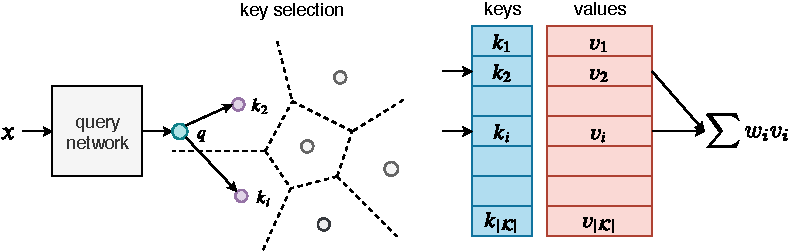
\includegraphics[width=1.0\linewidth]{figures/memory-crop.pdf}
    \caption{乘积记忆存储器的示意图\cite{Lample2019LargeML}}
    \label{fig:PKM}
\end{figure}

面对海量（例如百万级别）的密钥，穷举式的相似度计算是不可行的。为了高效地从中检索信息，PKM引入了“乘积量化”（Product Quantization）的思想来构建和查询密钥。具体来说，一个高维的密钥$k$被分解为两个低维子密钥$c_1$和$c_2$的拼接（concatenation），即$k = [c_1, c_2]$。整个密钥空间由两个较小的子密钥码本$C_1 \in \mathbb{R}^{N_s \times (d_k/2)}$和$C_2 \in \mathbb{R}^{N_s \times (d_k/2)}$的笛卡尔积隐式定义，其中$N_s = \sqrt{N}$是每个码本的大小，$d_k$是完整密钥的维度。这样，总的密钥数量可以达到$N = N_s^2$。

其选择过程分为两个阶段：
\begin{enumerate}
    \item \textbf{候选集生成}：对于一个输入$x$生成的查询向量$q$（同样被分解为$[q_1, q_2]$），模型首先在两个子码本中独立地进行快速的Top-$k_s$搜索，找出与$q_1$和$q_2$最相似的$k_s$个子密钥。
    \begin{gather}
        \mathcal{T}_1 = \text{TopK}_{k_s}(\{ q_1^T c_{1,i} \}_{i=1}^{N_s}) \\
        \mathcal{T}_2 = \text{TopK}_{k_s}(\{ q_2^T c_{2,j} \}_{j=1}^{N_s})
    \end{gather}
    其中$\mathcal{T}_1$和$\mathcal{T}_2$是选出的$k_s$个子密钥的索引集合。这两个集合中的子密钥组合起来，构成了一个包含$k_s^2$个完整密钥的候选集。理论上可以证明，与完整查询$q$最相似的Top-$k$密钥必定位于这个候选集中。
    \item \textbf{最终专家选择}：接下来，模型仅在这个小得多的候选集上计算完整的相似度得分，并从中选出最终的Top-$k$个密钥。对于候选集中的任意一个密钥$k_{ij} = [c_{1,i}, c_{2,j}]$（其中$i \in \mathcal{T}_1, j \in \mathcal{T}_2$），其与$q$的点积得分为$s_{ij} = q^T k_{ij} = q_1^T c_{1,i} + q_2^T c_{2,j}$。模型基于这$k_s^2$个得分选出最高的$k$个，其对应的索引集合记为$\mathcal{T}_{\text{final}}$。
\end{enumerate}

最终，模型的输出$y$是被选中的$k$个值向量$V_{ij}$的加权和，权重由这些最终得分经过softmax函数归一化得到：
\begin{equation}
    y = \sum_{(i,j) \in \mathcal{T}_{\text{final}}} \text{softmax}(\{s_{uv}\}_{(u,v) \in \mathcal{T}_{\text{final}}})_{ij} \cdot V_{ij}
\end{equation}
通过这种两阶段的搜索策略，PKM将检索的计算复杂度从与密钥总数$N$成正比（$O(N)$）降低到了与$N$的平方根成正比（$O(\sqrt{N})$），成功地将模型容量与计算开销解耦。

\subsection{PEER}
He等人提出的PEER（Parameter Efficient Expert Retrieval）\cite{He2024MixtureOA}模型在PKM的基础上迈出了关键一步，使其更符合“专家”的动态计算特性。PEER沿用了PKM的乘积密钥路由机制来实现高效的专家检索，但其核心创新在于：存储器中存储的不再是静态的“值”（value）向量，而是极度轻量化的“专家参数”（图\ref{fig:PEER}）。

\begin{figure}[h]
    \centering
    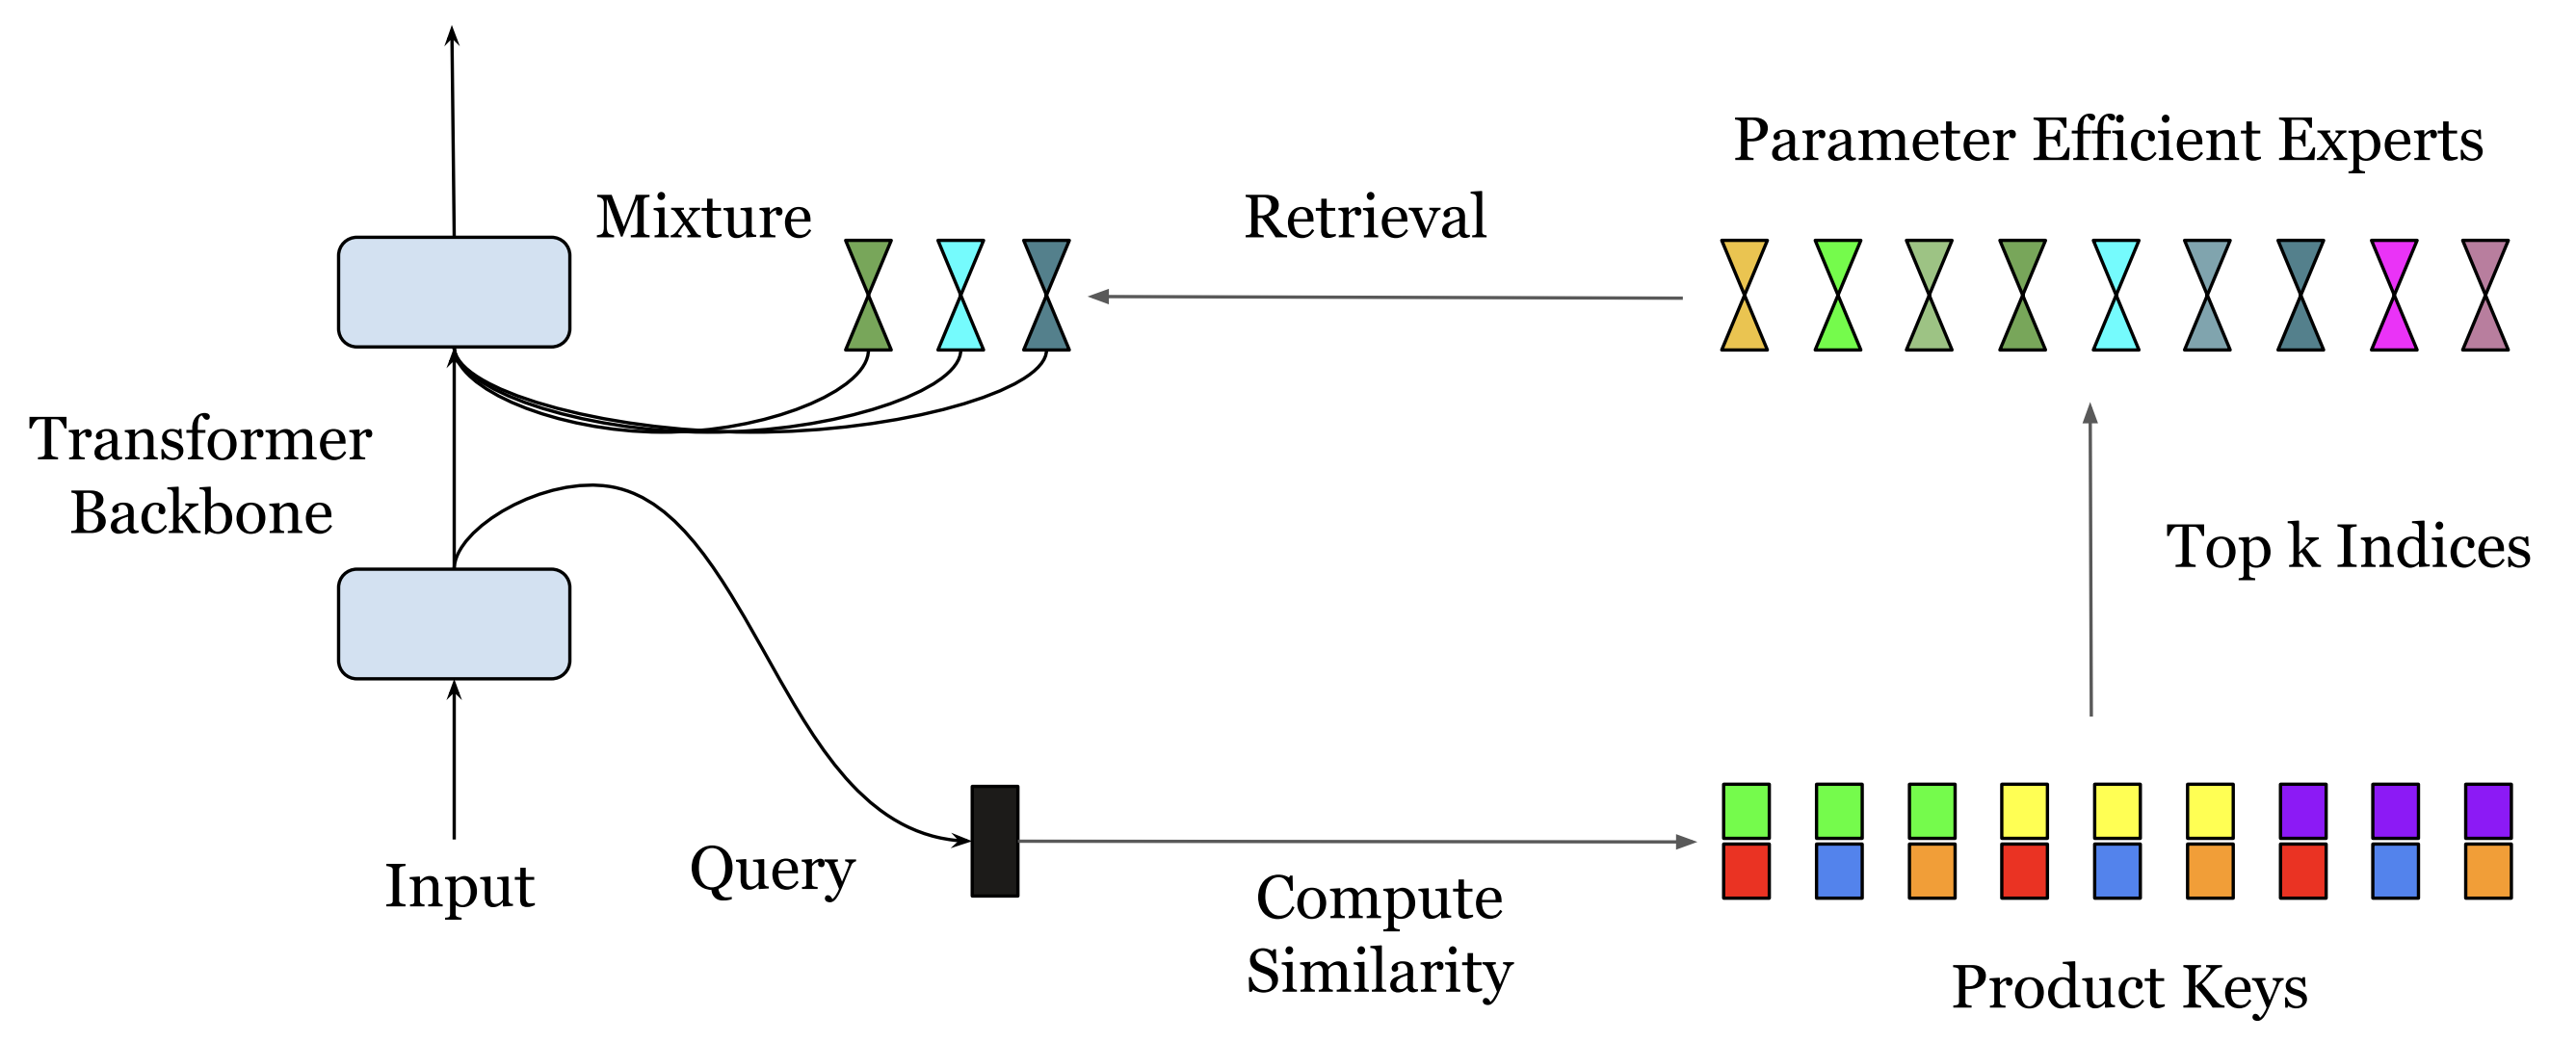
\includegraphics[width=1.0\linewidth]{figures/peer.jpg}
    \caption{PEER架构\cite{He2024MixtureOA}}
    \label{fig:PEER}
\end{figure}

具体来说，每个专家被实现为一个单神经元的多层感知机（MLP），其计算可以表示为：
\begin{equation}
    E_i(x) = \sigma(x\cdot u_i) v_i
\end{equation}
其中，$u_i$和$v_i$是专家的可学习参数（向量）。当一个输入$x$通过类似PKM的路由器检索到第$i$个专家时，模型取回的是参数$u_i$和$v_i$，并利用它们对$x$进行计算。这种设计使得每个专家的行为是输入依赖的（input-dependent），而不仅仅是返回一个固定的值，从而更贴近“专家”的本质。

PEER将专家粒度降至单个神经元，成功构建了一个拥有一百万个微型专家的混合专家模型，并在实验中证明了其在性能与计算成本权衡方面的优越性，为极大化专家数量的思路提供了有力支持。

\subsection{Ultra-Sparse Memory Network (UltraMem)}
Huang等人提出的Ultra-Sparse Memory Network (UltraMem)\cite{Huang2024UltraSparseMN} 旨在进一步解决PKM和PEER等架构在扩展到更大规模时遇到的性能和效率瓶颈。UltraMem通过引入更先进的组件和并行策略，显著提升了模型的表达能力和训练效率。其核心改进包括塔克分解查询密钥检索（Tucker Decomposed Query-Key Retrieval, TDQKR）、隐式值扩展（Implicit Value Expansion, IVE）以及一种高效的并行计算策略。

\subsubsection{塔克分解查询密钥检索 (TDQKR)}
TDQKR（图\ref{fig:tucker}）是对PKM中简单的加性评分机制的重大升级。PKM假设行、列子密钥的贡献是独立的（$s_{ij} = s_i + s_j$），这限制了路由的表达能力，并可能导致“拓扑偏差”（即Top-2密钥很可能与Top-1密钥在同一行或同一列）。TDQKR通过引入一个可学习的、低秩的“塔克核心”（Tucker core）张量$C \in \mathbb{R}^{r \times r}$来捕捉子密钥之间更复杂的乘性交互关系，其中$r$是塔克分解的秩。其得分矩阵的计算方式可以近似为：
\begin{equation}
    S_{\text{grid}} \approx \sigma_{\text{topM}}(S_{\text{row}}^T \times C \times S_{\text{col}})
\end{equation}
这里，$S_{\text{row}}$和$S_{\text{col}}$是查询与子密钥交互后得到的分数张量。这种设计允许模型学习到更灵活、更具表达力的路由模式，打破了简单的加性组合的局限，从而提高了专家选择的准确性。

\begin{figure}[h]
    \centering
    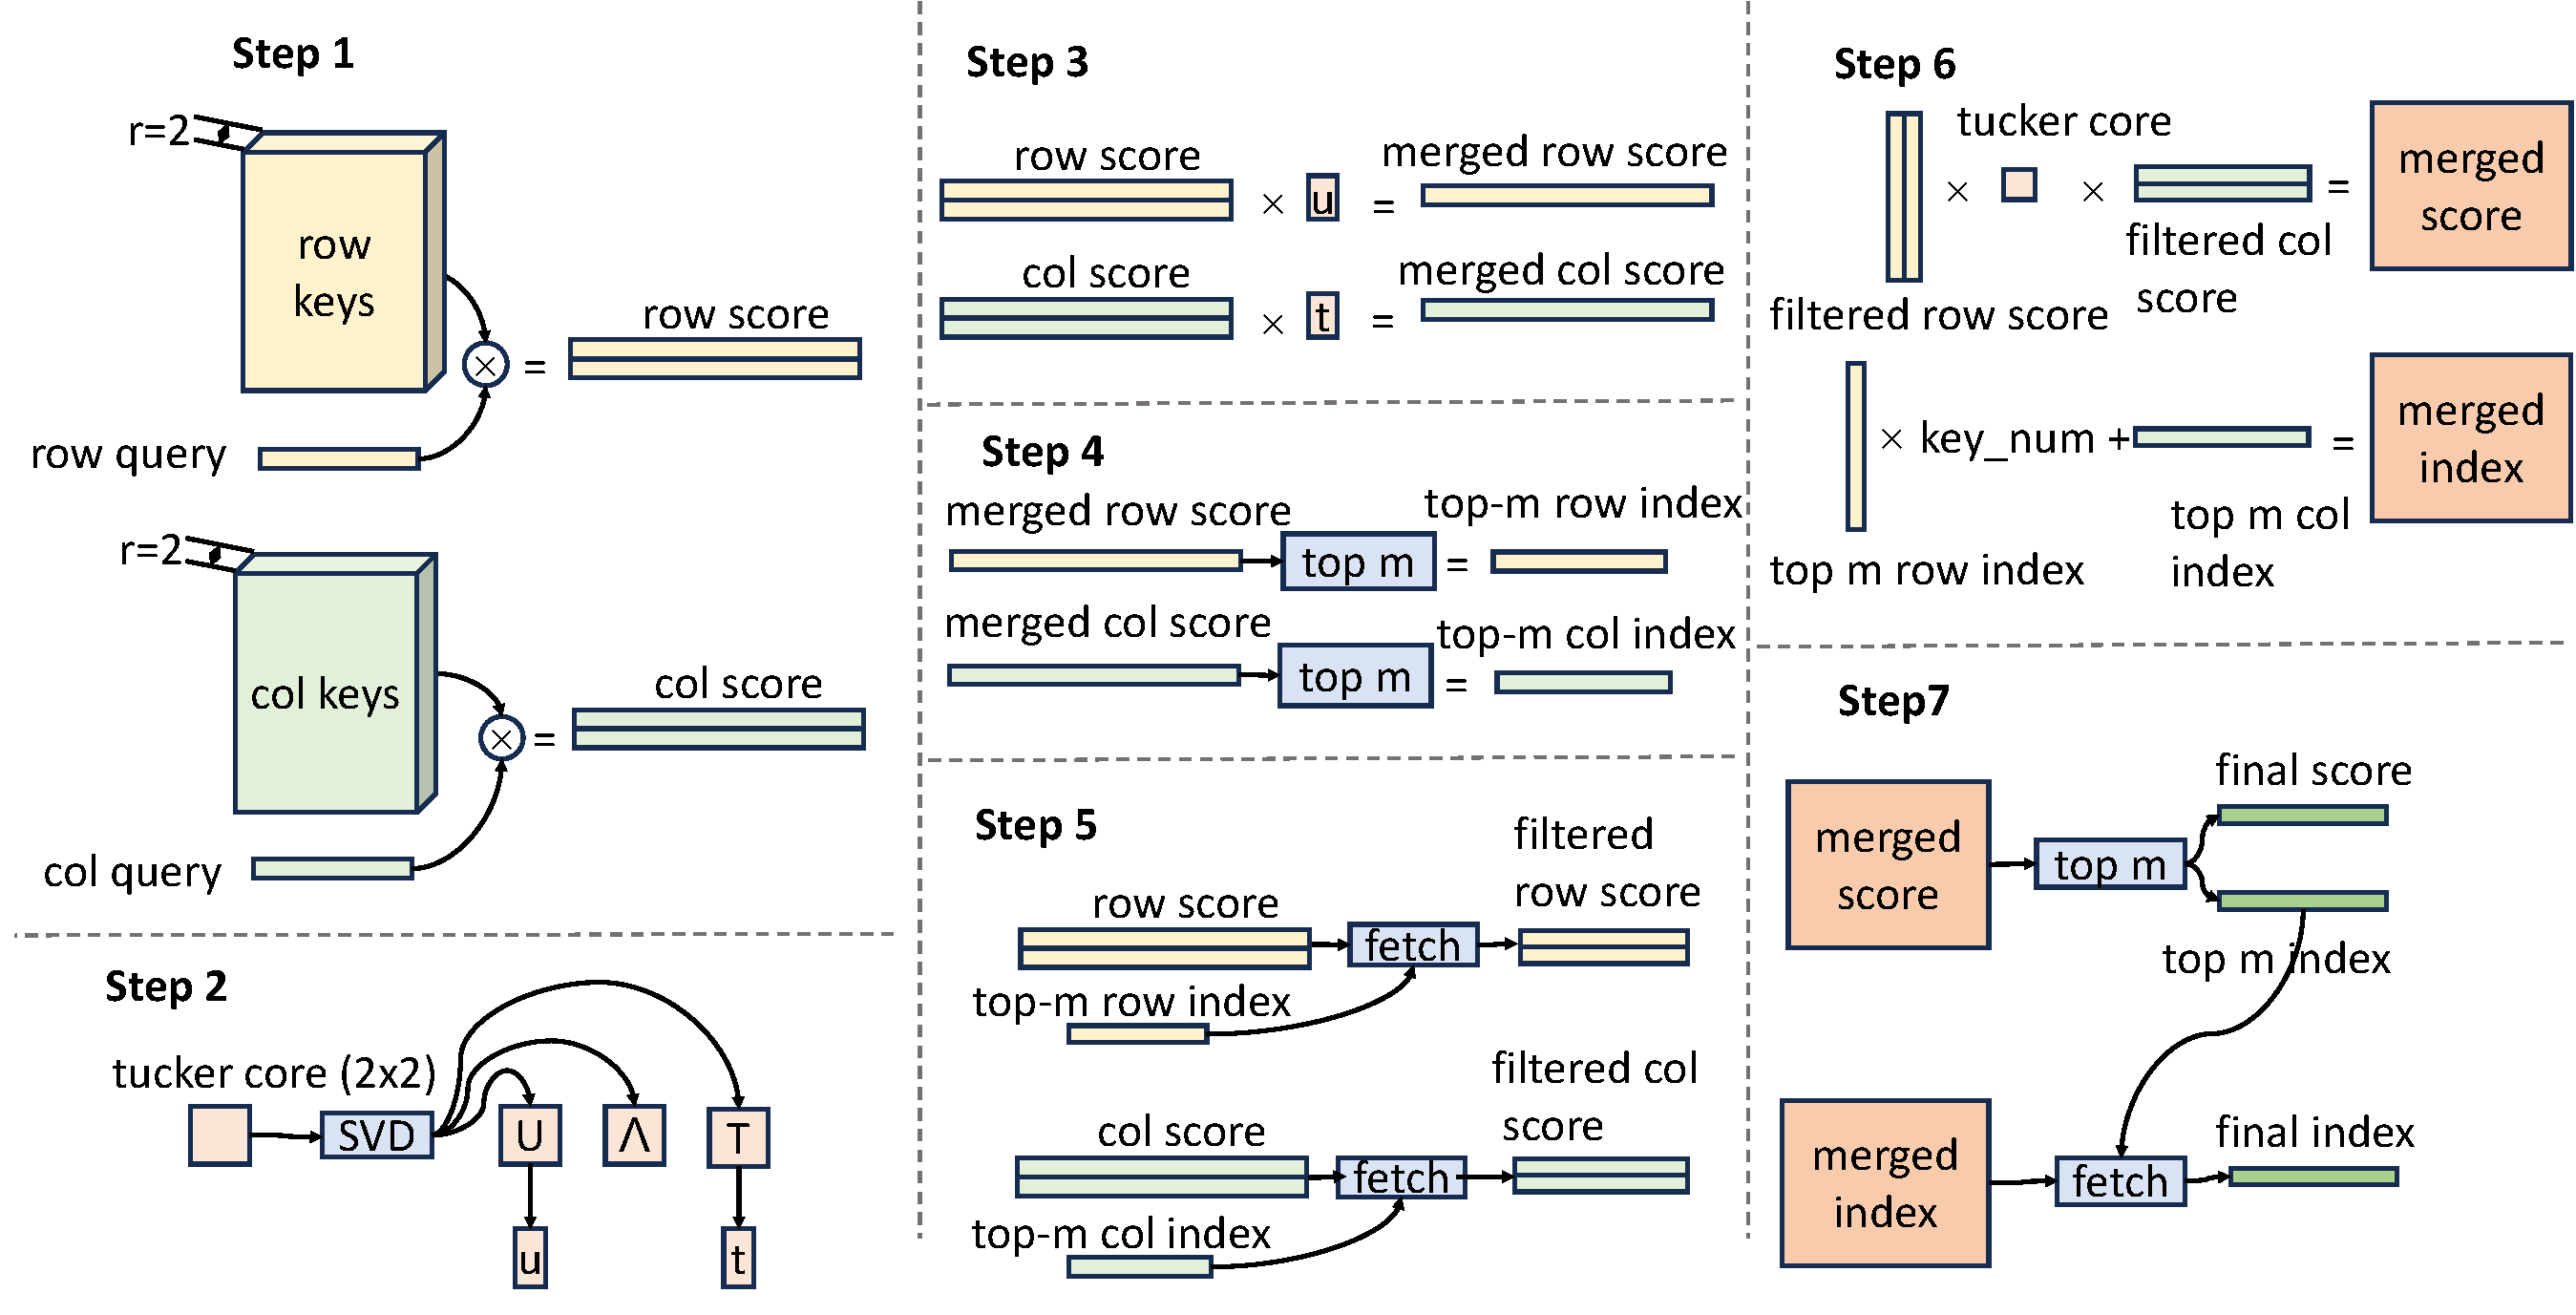
\includegraphics[width=1.0\linewidth]{figures/tucker_big.pdf}
    \caption{塔克分解查询密钥检索 (TDQKR)\cite{Huang2024UltraSparseMN}}
    \label{fig:tucker}
\end{figure}

\subsubsection{隐式值扩展 (IVE)}
IVE（图\ref{fig:ive}）是一种在不显著增加物理存储和访存开销的前提下，虚拟地扩大模型容量的技术。其动机是在保持计算效率的同时，进一步增加参数量。IVE将物理存储的值向量$V$（较小）通过一组$E$个可学习的线性投影矩阵$\{W_p\}_{p=1}^E$动态地生成多个“虚拟值块”$\tilde{V}_p = V W_p$。最终的输出是对这些虚拟值块的加权求和，计算可以被优化为“按需”进行：
\begin{equation}
o = \sum_{p=1}^E \tilde{V}_p^T \hat{s}_p = \sum_{p=1}^E W_p^T(V^T \hat{s}_p)
\end{equation}
其中$\hat{s}_p$是对应第$p$个虚拟块的得分。这种方式避免了在内存中实例化所有巨大的虚拟值参数，而是在计算时动态生成，从而以极小的额外计算代价实现了参数量的大幅扩展。

\begin{figure}[h]
    \centering
    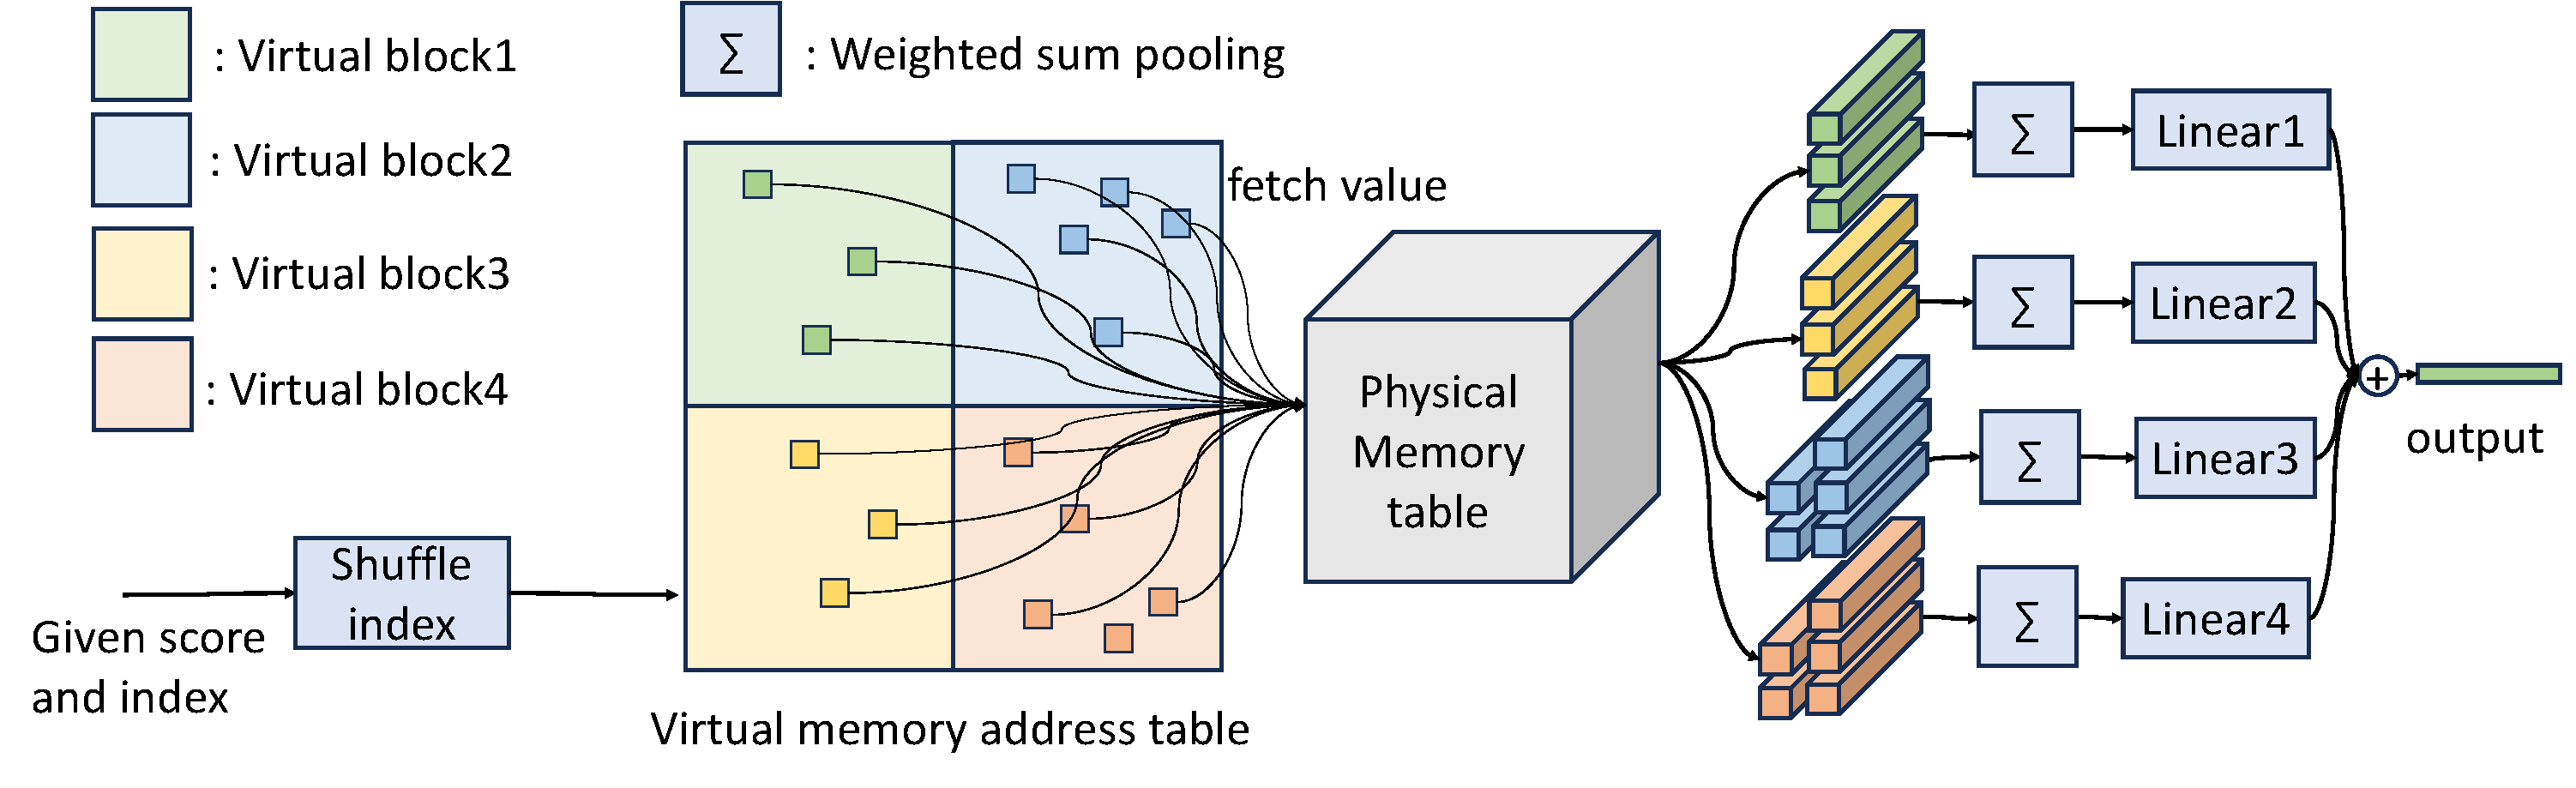
\includegraphics[width=1.0\linewidth]{figures/value_proj_big.pdf}
    \caption{隐式值扩展 (IVE)\cite{Huang2024UltraSparseMN}}
    \label{fig:ive}
\end{figure}

\subsubsection{并行计算策略}
为了提升训练效率，UltraMem采用了一种巧妙的并行策略。它并非将一个巨大的记忆层集中放置在模型某处，而是将多个较小的记忆层分散地插入到Transformer的不同块之间，形成一种“交错式”（interleaved）的架构（图\ref{fig:ultra_parallel}）。

\begin{figure}[h]
    \centering
    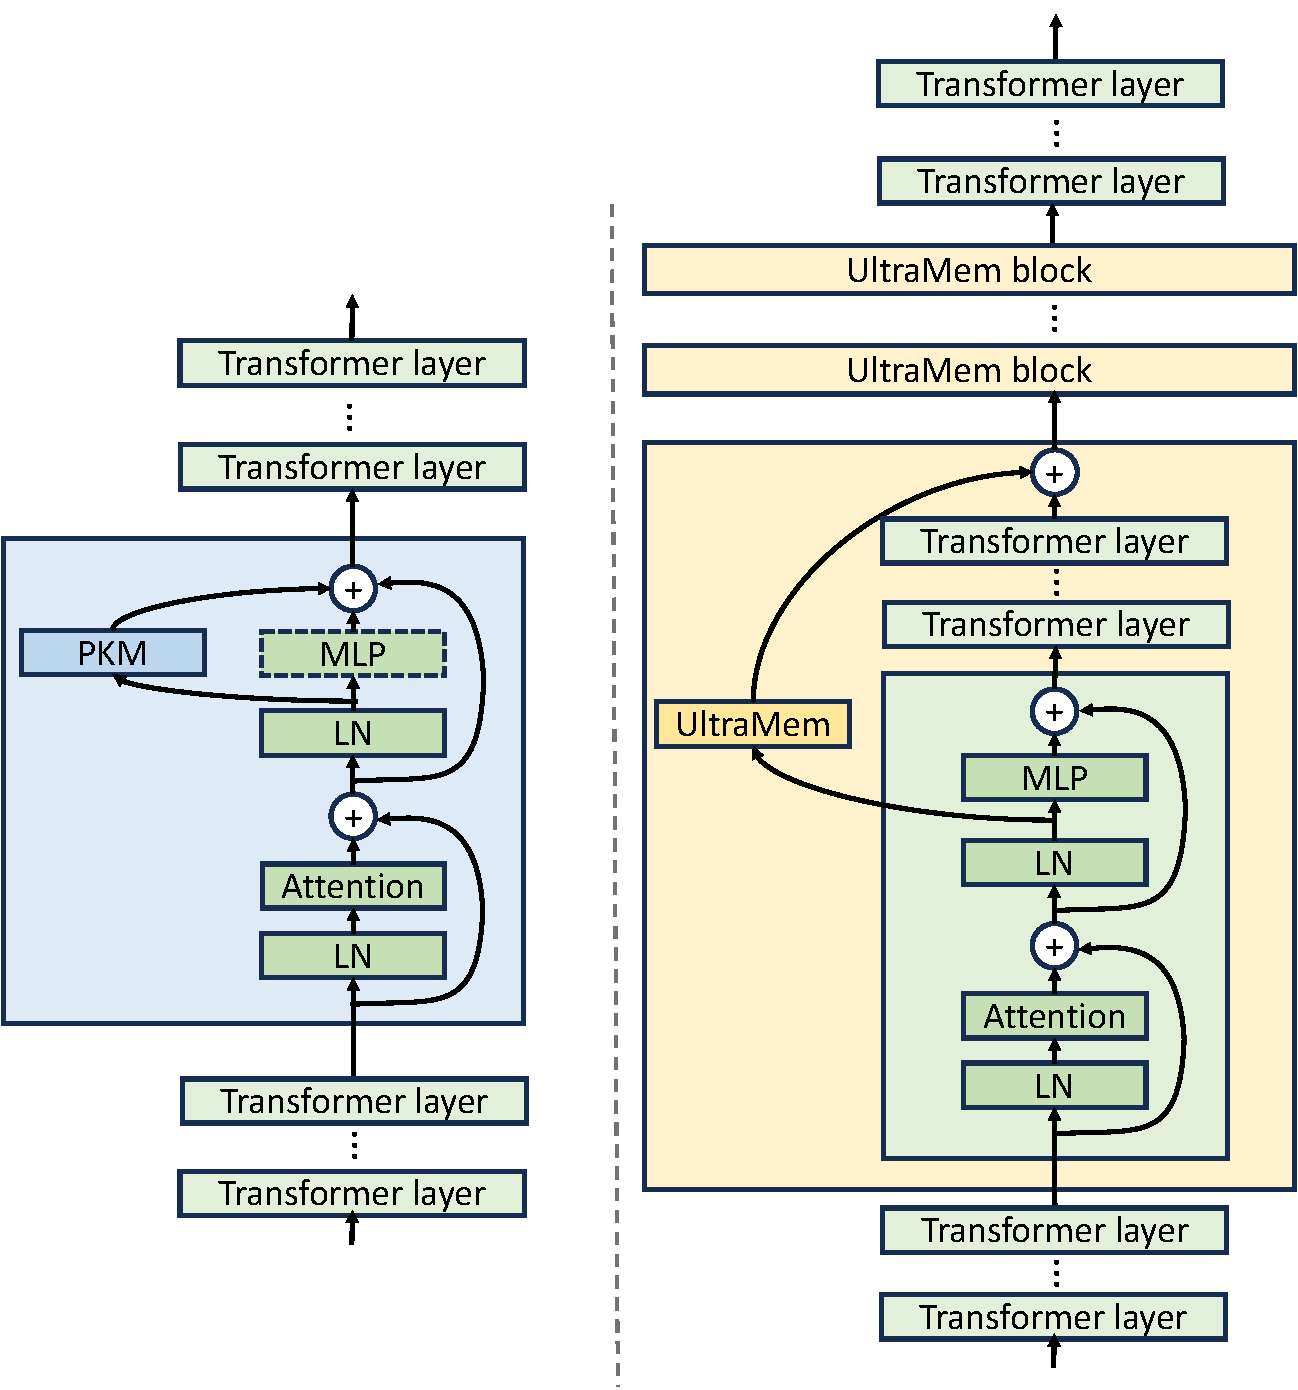
\includegraphics[width=0.7\linewidth]{figures/overall_structure.pdf}
    \caption{UltraMem的并行策略\cite{Huang2024UltraSparseMN}}
    \label{fig:ultra_parallel}
\end{figure}

这种策略的核心优势在于利用了不同类型计算层的硬件特性。标准的Transformer层（如自注意力和FFN）是“计算密集型”（compute-bound）的，其瓶颈在于处理器的浮点运算速度。而UltraMem的记忆层主要是“内存带宽密集型”（memory-bound）的，其瓶颈在于从GPU内存中读取大量密钥和值。

通过将这两种不同特性的层交错放置，可以实现\textbf{计算与访存的重叠（overlap）}。当GPU为一个Transformer块执行计算密集型操作时，数据预取机制可以异步地为下一个UltraMem层从内存中加载数据。反之，当GPU等待内存数据访问时，它可以处理其他计算任务。这种异步执行的流水线模式能够有效隐藏内存访问延迟，提升GPU的整体利用率，从而显著加快模型的训练速度。

\subsubsection{UltraMemV2}
在 UltraMem 的基础上，Huang 等人进一步提出了 UltraMemV2\cite{Huang2025UltraMemV2MN}（图\ref{fig:ultra_mem_v2}），其目标是使基于记忆的极细粒度专家架构在性能上能够与业界顶尖的、拥有 8 个激活专家的传统混合专家模型相媲美。为了实现这一目标，UltraMemV2 进行了一系列关键的架构和训练策略改进，成功地弥合了记忆层架构与主流稀疏模型之间的性能鸿沟。

\begin{figure}[h]
    \centering
    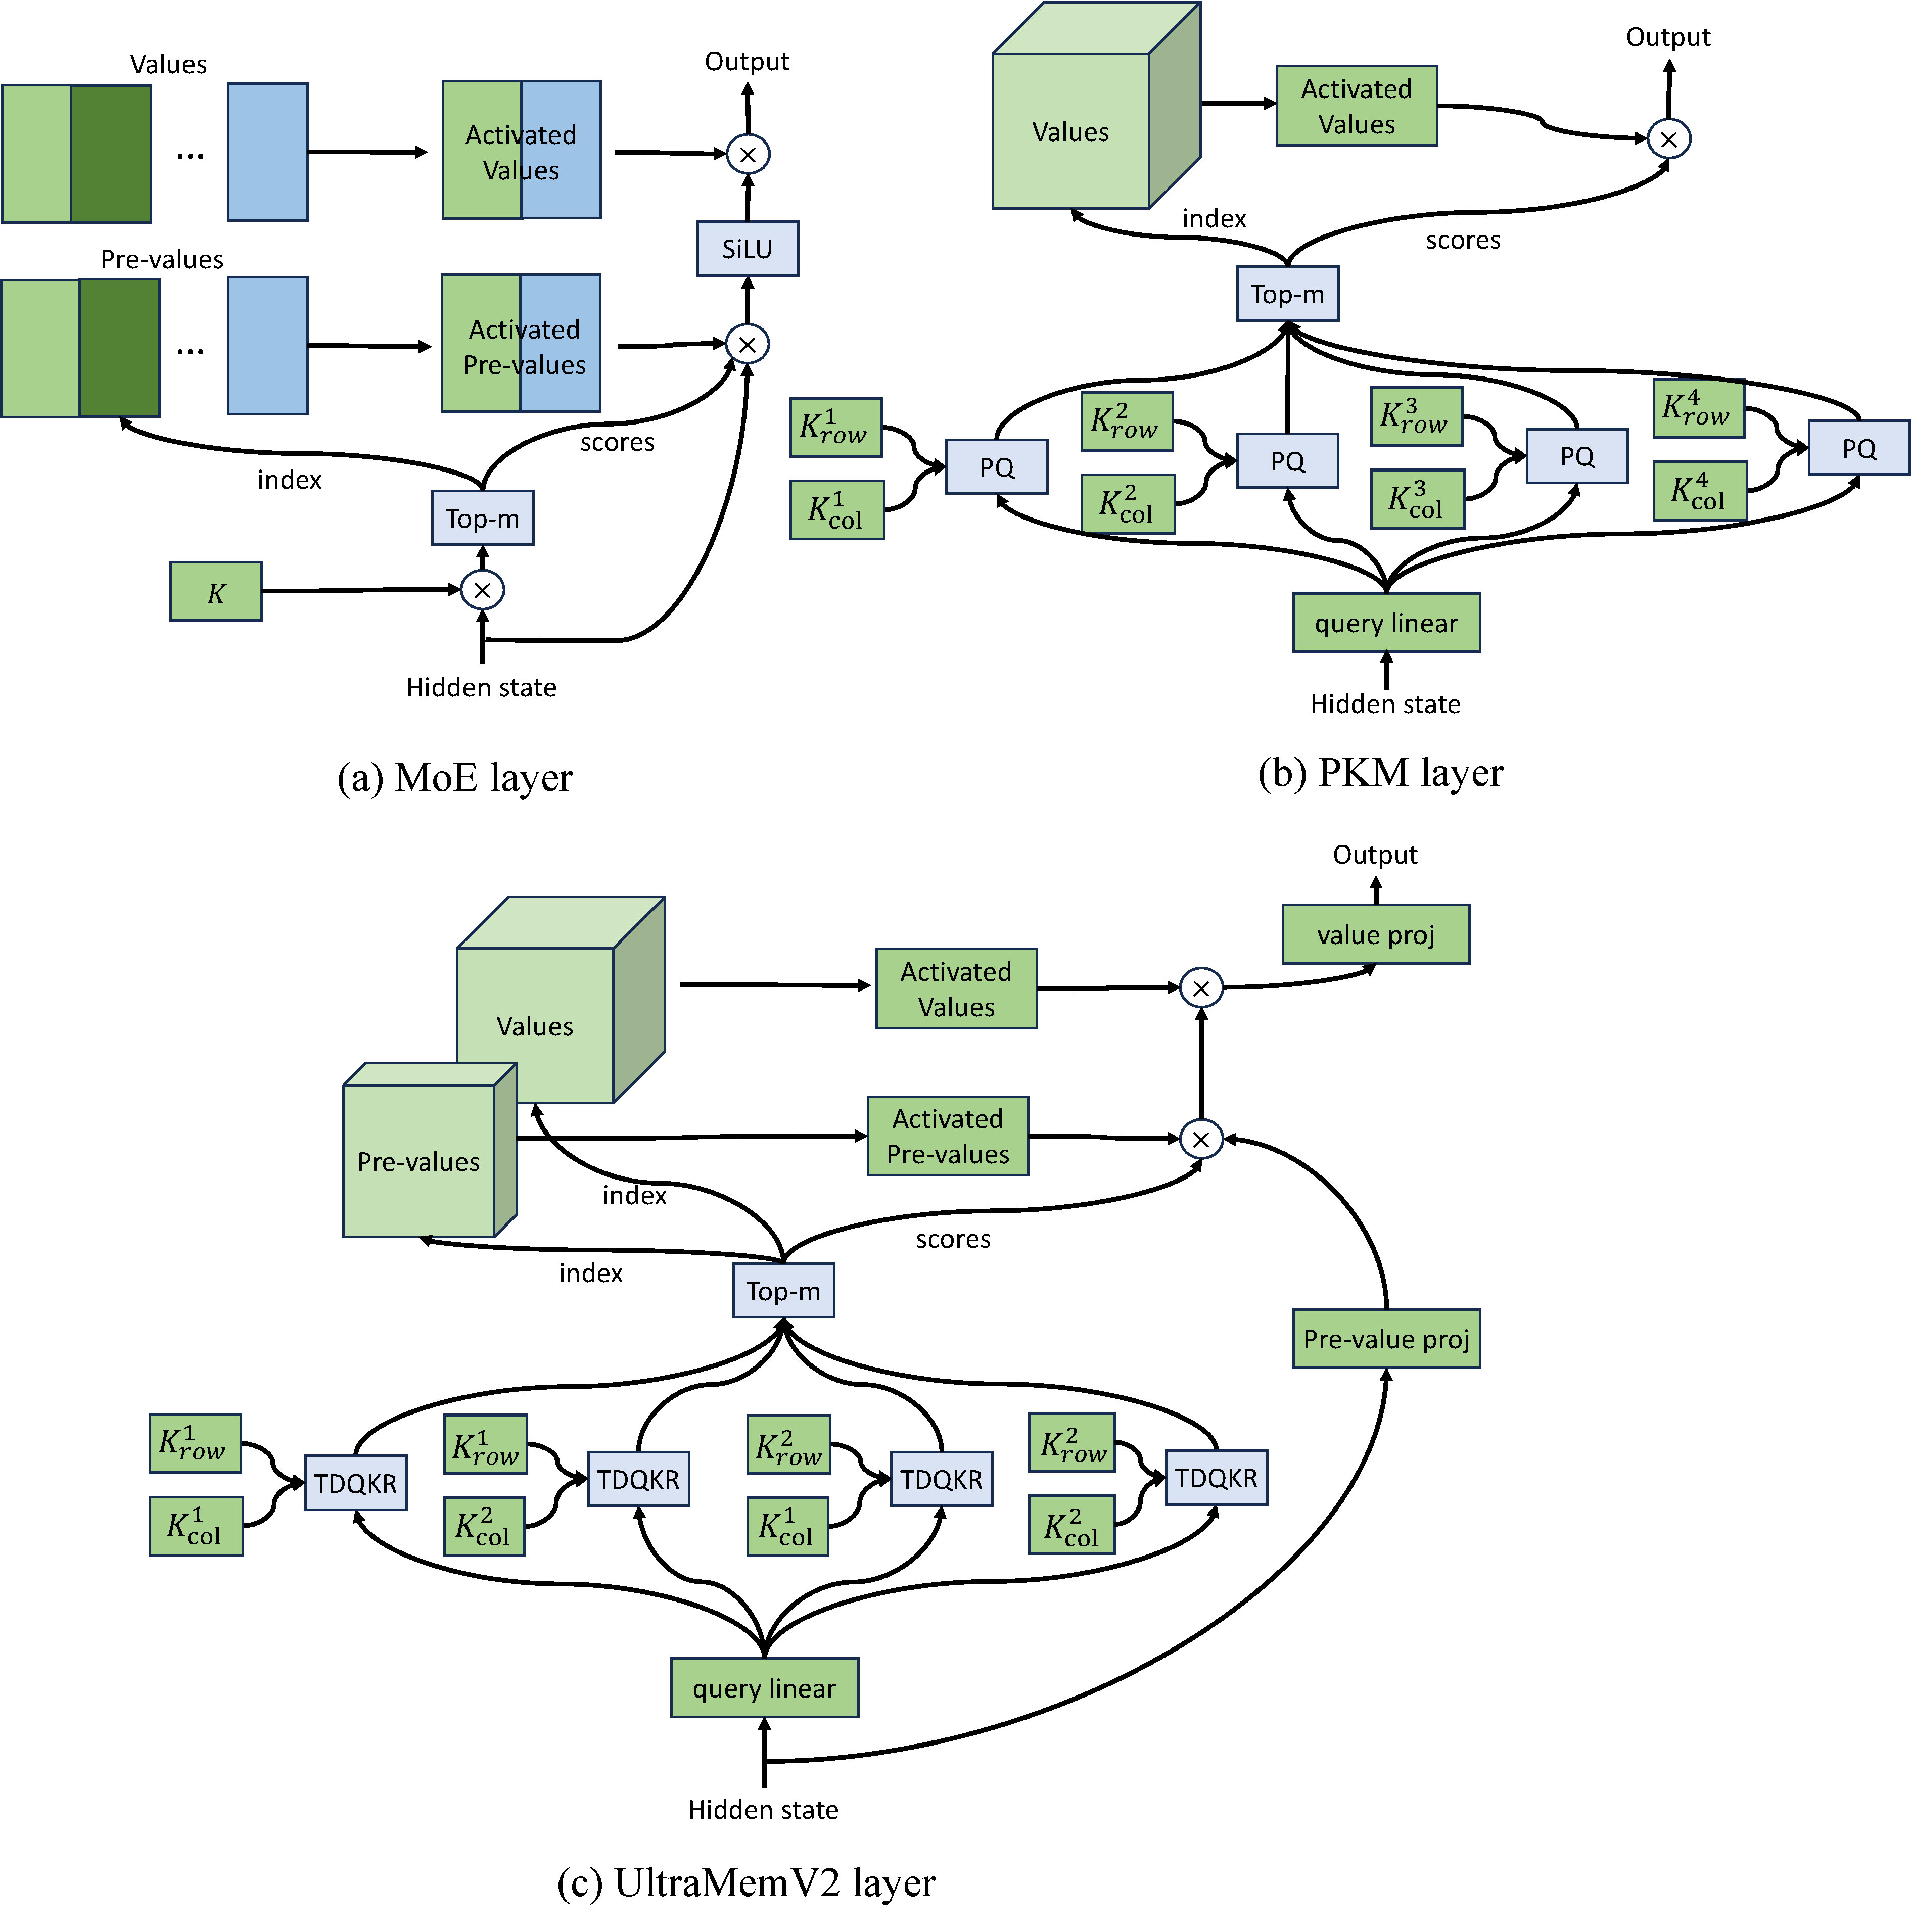
\includegraphics[width=1.0\linewidth]{figures/3structure.pdf}
    \caption{UltraMemV2和先前工作的对比\cite{Huang2025UltraMemV2MN}}
    \label{fig:ultra_mem_v2}
\end{figure}

UltraMemV2 的核心思想是通过五项关键改进来提升模型性能与效率：

\begin{enumerate}
    \item \textbf{架构集成（Architectural Integration）：} 将记忆层更紧密地集成到模型中。不同于以往模型仅在部分层插入记忆模块，UltraMemV2 在每一个 Transformer 块中都包含一个 UltraMemV2 层，使其与稠密计算部分深度融合，从而增加了稀疏参数的参与度。

    \item \textbf{简化的值扩展（Simplified Value Expansion）：} 对 UltraMem 中的隐式值扩展（IVE）机制进行简化。原始的 IVE 为每个虚拟内存块使用独立的线性投影层，这增加了非计算操作的开销。UltraMemV2 将其简化为使用单个共享的线性投影层来处理所有激活的值，如公式 \ref{eq:ultramemv2_ive} 所示。这一改动在保留模型容量的同时，显著提升了推理速度。
    \begin{equation}
        \boldsymbol{y} = \boldsymbol{W}_{\text{shared}} (\boldsymbol{V}^\top \hat{\boldsymbol{s}})
        \label{eq:ultramemv2_ive}
    \end{equation}
    其中 $\hat{\boldsymbol{s}}$ 是经过路由和排序后的得分向量，$\boldsymbol{V}$ 是物理值存储，$\boldsymbol{W}_{\text{shared}}$ 是所有虚拟块共享的单个线性投影。

    \item \textbf{类专家的值处理（Expert-like Value Processing）：} 借鉴 PEER 的思想，采用基于前馈网络的值处理方式。传统记忆网络检索的是静态的值向量，而 UltraMemV2 将其替换为动态的、依赖于输入的单神经元计算。具体而言，模型检索的不再是值向量本身，而是一个“预值”（pre-value）矩阵 $\boldsymbol{P}$。最终的输出通过一个前馈网络计算得出，如公式 \ref{eq:ultramemv2_peer} 所示。这种设计极大地增强了模型的表达能力。
    \begin{equation}
        \boldsymbol{y} = \boldsymbol{W}^\top (\boldsymbol{V}^\top \otimes ((\boldsymbol{P}\boldsymbol{x}) \otimes \hat{\boldsymbol{s}}))
        \label{eq:ultramemv2_peer}
    \end{equation}
    其中 $\boldsymbol{x}$ 是输入词元的表征，$\otimes$ 表示逐元素乘法。这一改动使得每个被激活的“专家”都能够根据当前输入动态地调整其输出。

    \item \textbf{优化的参数初始化（Optimized Initialization）：} 针对新架构设计了更符合理论的参数初始化方案。为了避免在训练大规模模型时可能出现的不稳定问题，UltraMemV2 的初始化策略确保了记忆层的输出激活方差与标准前馈网络层的方差保持一致，从而显著提升了训练的稳定性。

    \item \textbf{计算比例再平衡（Computational Rebalancing）：} 重新调整了记忆检索与前馈网络之间的计算量比例。通过实验分析，找到了一个最优的平衡点，以优化整体模型的性能。
\end{enumerate}

通过这些改进，UltraMemV2 成功地在各项基准测试中达到了与 8-expert 混合专家模型相当的性能，尤其在长上下文和记忆密集型任务上展现出优越性。这标志着极细粒度专家架构已发展成为一种兼具高效推理与强大性能的、有竞争力的稀疏模型方案。

% \subsection{专家选择的软性化 (Soft Expert Selection)}
% 与Top-k的“硬性”选择不同，一些研究探索了软性的路由机制，即每个词元与所有专家都进行交互，但交互的权重是稀疏的。这类方法虽然理论上更具表达力，但通常难以在现代硬件上实现高效计算，因此应用较少。
% FROM SPARSE TO SOFT MIXTURES OF EXPERTS
% Soft Merging of Experts with Adaptive Routing


% % MOA / MOM / MOR / MOD 
% [这里补充 MoH: Multi-Head Attention as Mixture-of-Head Attention]

% % topp; expert choice; Dynamic Mixture of Experts DYNMoE

% % 极细粒度的moe (PKM, peer / 字节的supermoe还是叫什么的)
% Large Memory Layers with Product Keys
% Mixture of A Million Experts
% ULTRA-SPARSE MEMORY NETWORK
% UltraMemV2: Memory Networks Scaling to 120B
% Parameters with Superior Long-Context Learning


% dense 2 sparse / sparse 2 dense之类的工作 https://arxiv.org/pdf/2410.08589

        \chapter{个人研究进展}
\label{chap:personal_research}

在对混合专家模型（Mixture-of-Experts, MoE）架构与训练策略进行广泛而深入的调研基础上，我们识别出负载均衡（Load Balancing）是制约其性能和训练稳定性的核心挑战之一。经典的负载均衡策略，如第\ref{sec:aux_loss}节所述，通常依赖于一个辅助损失函数（Auxiliary Loss）来鼓励路由器（Router）将计算负载均匀地分配给所有专家（Experts）。然而，这种方法引入了一个固有的权衡难题：一个较弱的辅助损失可能无法有效解决负载不均衡问题，甚至导致部分专家训练不足，发生“路由坍缩”（Routing Collapse）现象；而一个较强的辅助损失则会产生不容忽视的干扰梯度（Interference Gradients），这些梯度与模型主要的语言建模目标相冲突，从而损害模型的最终性能。

为了打破这种“性能-均衡”的困境，我们进行了深入的探索，并提出了一种创新的、无需辅助损失的负载均衡策略，我们将其命名为\textbf{无辅助损失均衡（Auxiliary-Loss-Free Balancing）} \cite{Wang2024AuxiliaryLossFreeLB}。本章将详细阐述该策略的核心思想、算法设计、实验验证与分析。这项工作旨在为大规模混合专家模型的训练提供一种更高效、更稳定的负载均衡解决方案。

\section{动机：辅助损失的困境}
\label{sec:motivation_dilemma}

如第\ref{sec:aux_loss}节所述，现有的混合专家模型广泛采用辅助损失函数来引导负载均衡。该损失函数通常定义为：
\begin{equation}
    L_{\text{Balance}} = \alpha \cdot N \sum_{i=1}^{N} (f_i \cdot P_i)
\end{equation}
其中，$\alpha$ 是控制均衡强度的超参数，$N$ 是专家总数，$f_i$ 是路由到第 $i$ 个专家的词元（Token）比例，$P_i$ 是第 $i$ 个专家获得的平均门控权重（Gating Weights）。

这个辅助损失项虽然能够促进负载均衡，但也作为一个正则化项，引入了与主任务（如语言建模）无关的梯度。如图\ref{fig:dilemma_balance_performance}所示，超参数 $\alpha$ 的选择直接导致了模型性能和负载均衡之间的两难局面。当 $\alpha$ 值较小（例如 $10^{-4}$）时，虽然模型性能较好，但负载均衡效果差，容易导致路由坍缩。相反，当 $\alpha$ 值较大（例如 $10^{-2}$）时，负载均衡（以第\ref{sec:ep_and_lb}节中提及的最大负载违规率衡量）得到保证，但模型的性能（以困惑度 Perplexity 衡量）会显著下降。

\begin{figure}[h]
    \centering
    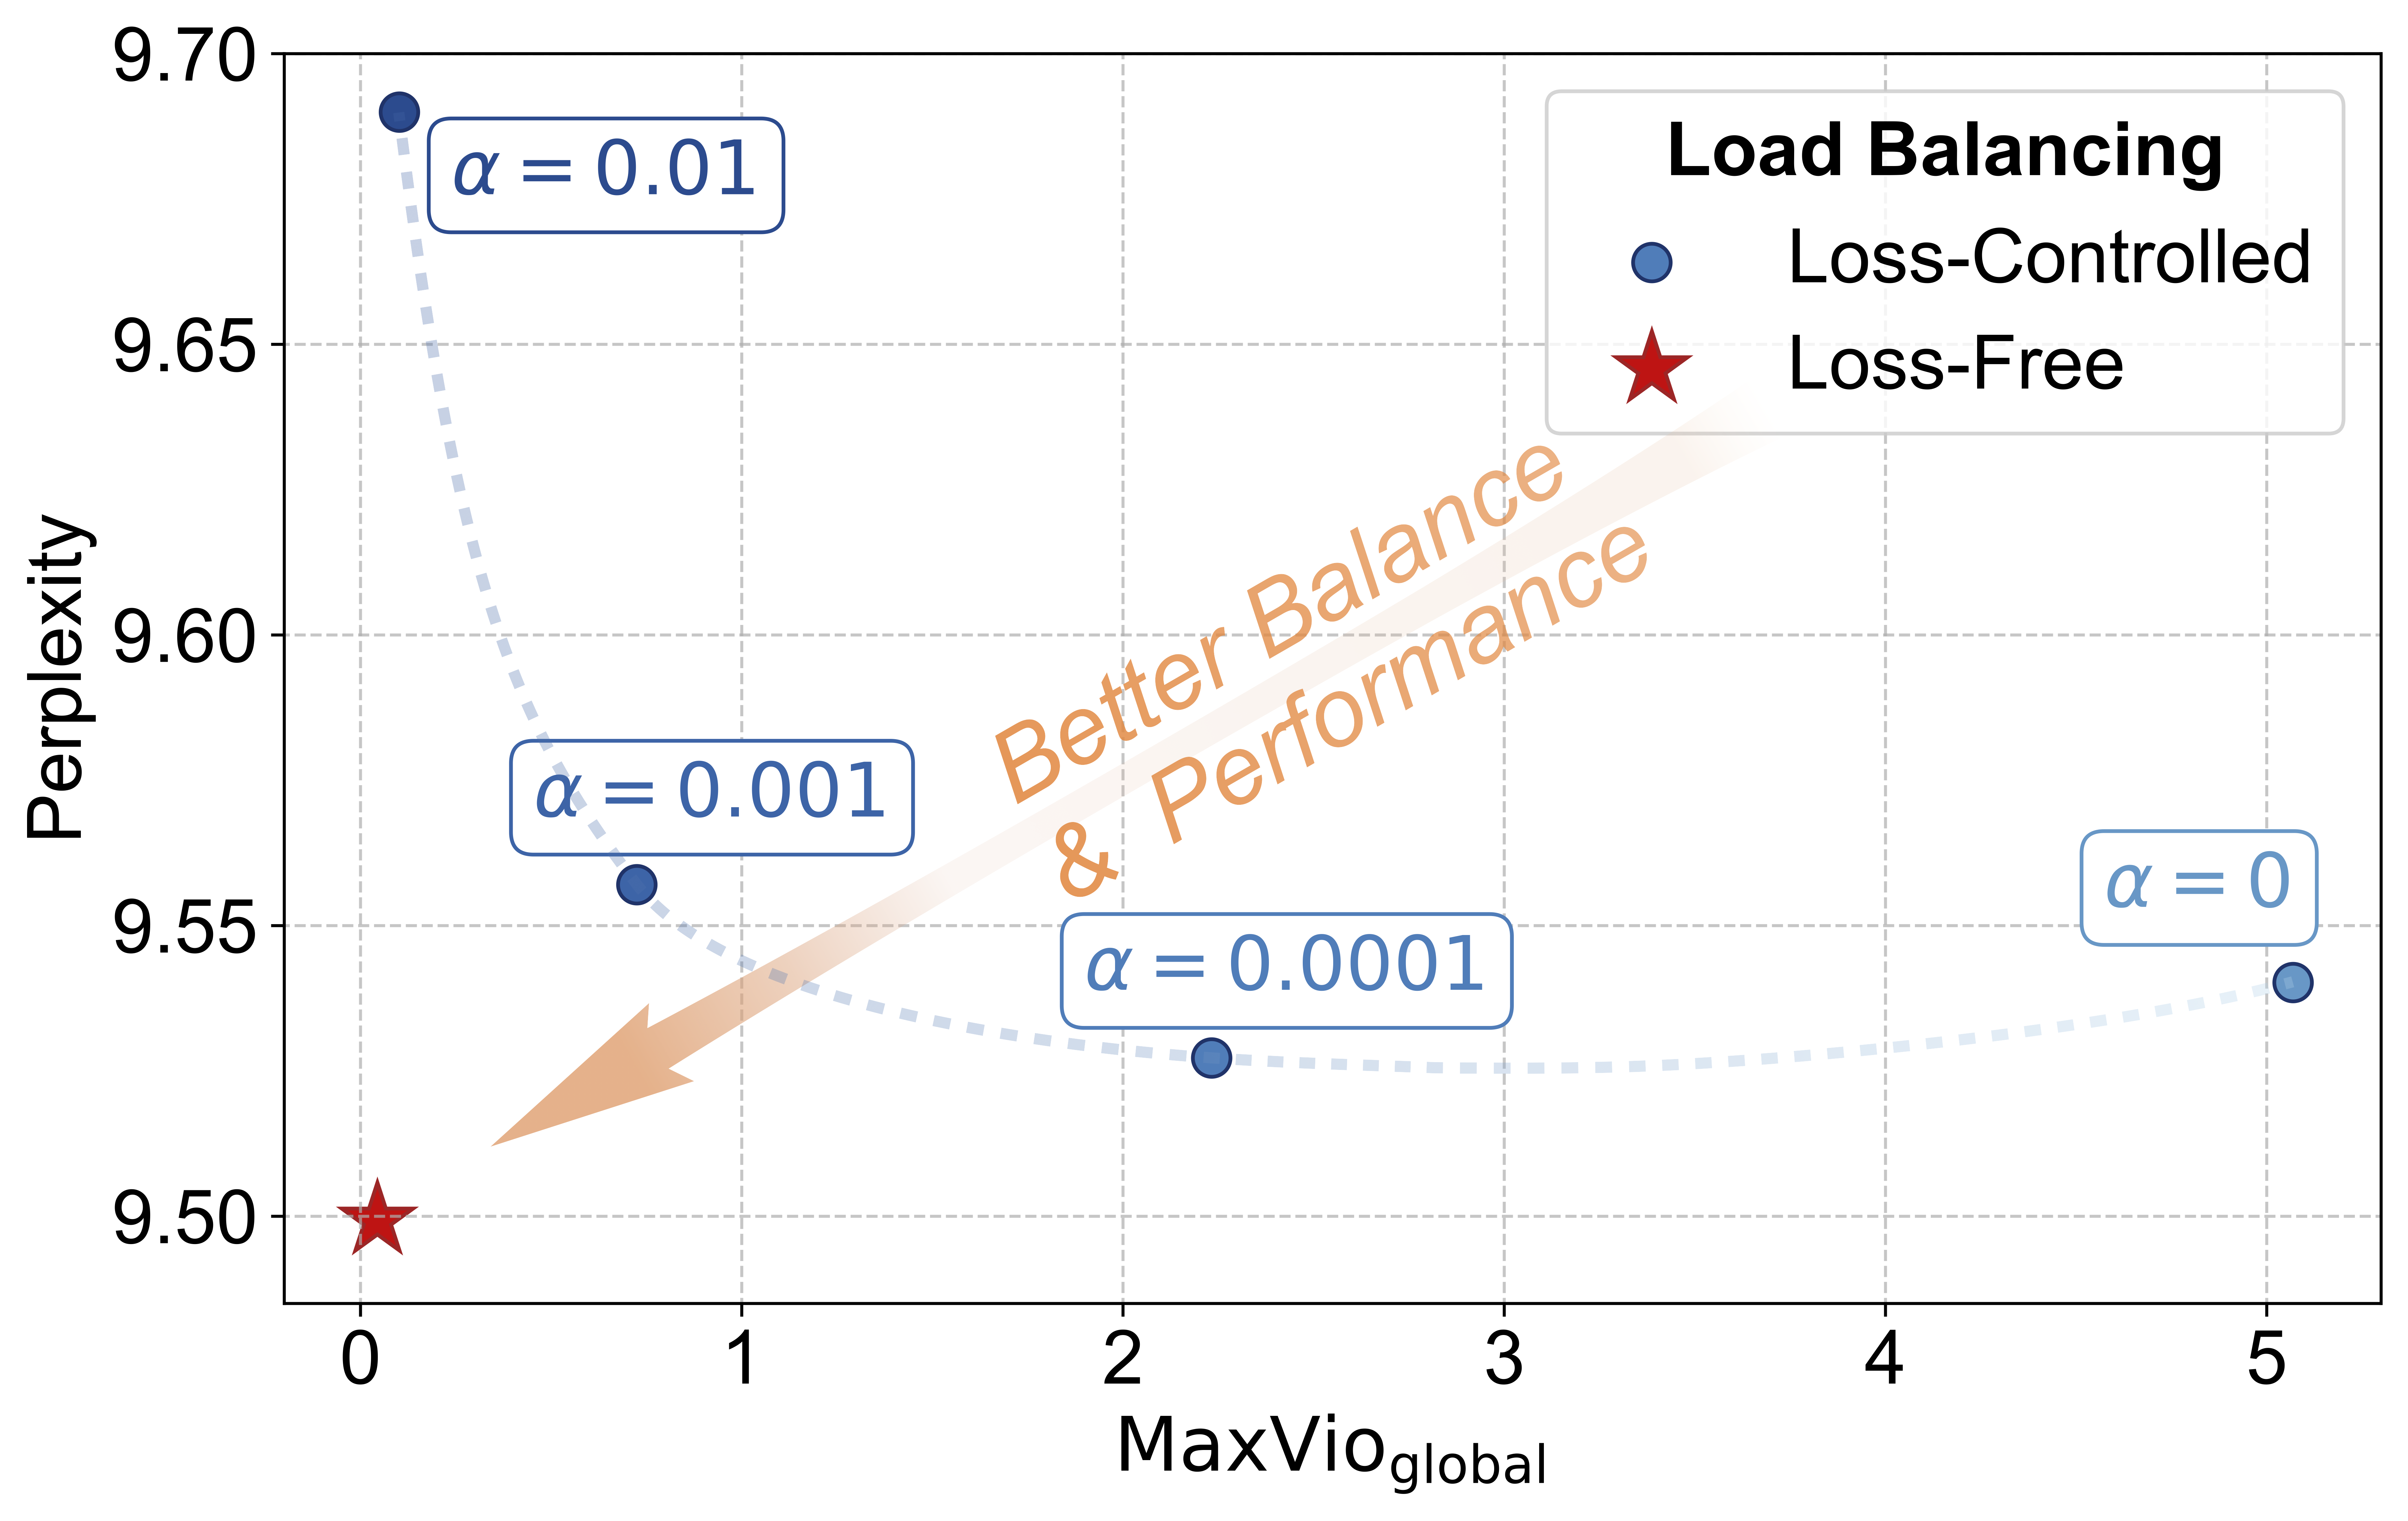
\includegraphics[width=0.8\textwidth]{figures/my_paper/balance_mv_perplexity_new_new.png}
    \caption{辅助损失控制下的负载均衡与模型性能困境。我们的无辅助损失均衡方法（红色星号）成功地打破了这一困境，同时实现了更优的性能和更好的负载均衡。}
    \label{fig:dilemma_balance_performance}
\end{figure}

这种固有的冲突表明，基于辅助损失的负载均衡策略可能并非最优解。理想的策略应该能够在不干扰主任务训练的前提下，直接且有效地控制专家负载。正是基于这一动机，我们设计了无辅助损失均衡策略。

% unfinished

\section{无辅助损失均衡（Auxiliary-Loss-Free Balancing）策略}
\label{sec:loss_free_balancing}

无辅助损失均衡策略的核心思想是：\textbf{不通过损失函数和梯度反向传播来间接“惩罚”不均衡，而是通过直接调整路由过程中的专家得分来实现主动“引导”均衡}。具体而言，我们在路由器计算出每个专家的原始路由得分（Routing Scores）之后，但在进行 Top-K 选择之前，为每个专家引入一个可动态调整的偏置项（Bias Term）。

\subsection{算法原理}

在每个训练步骤中，无辅助损失均衡策略包含两个核心环节：带偏置的专家选择和偏置项的动态更新。其工作流程如图 \ref{fig:lfb_workflow} 所示。

\begin{figure}[h]
    \centering
    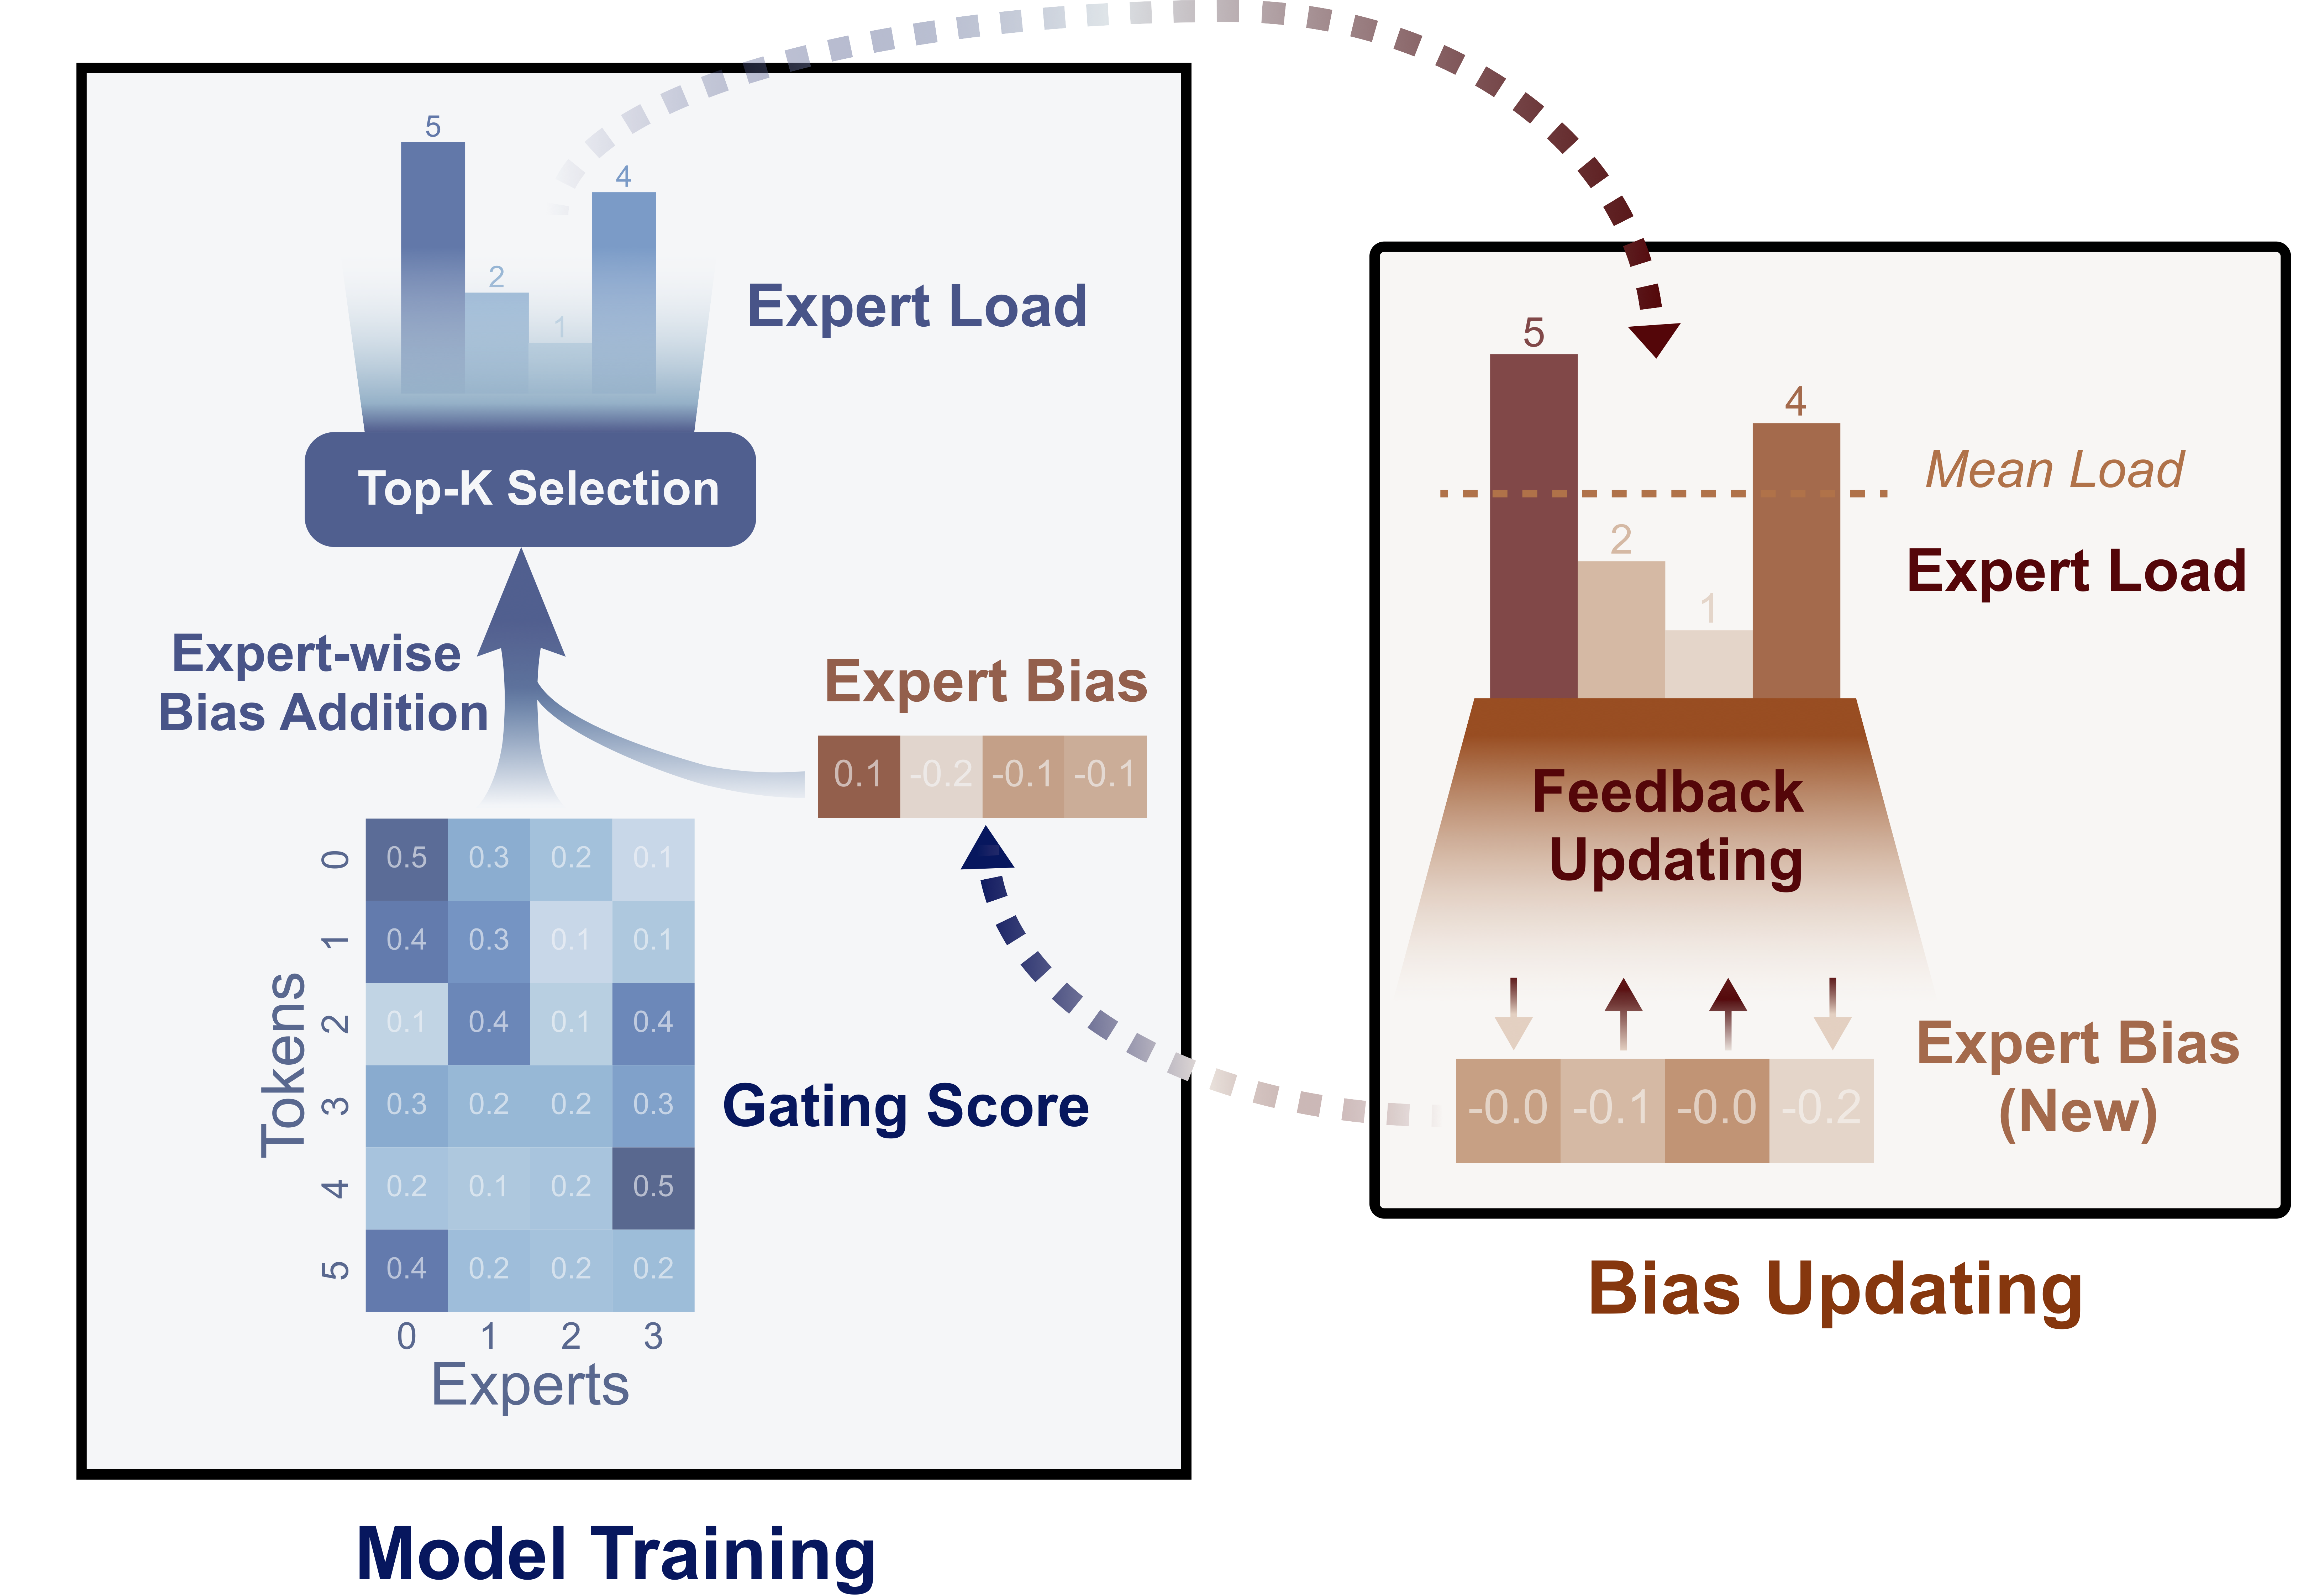
\includegraphics[width=0.9\textwidth]{figures/my_paper/figure_815.png}
    \caption{无辅助损失均衡策略的工作流程示意图。在每个训练步骤中，模型首先根据带有偏置的门控分数选择专家，然后在该步骤结束后，根据最近的专家负载情况反馈更新偏置项。}
    \label{fig:lfb_workflow}
\end{figure}

\paragraph{带偏置的专家选择}
对于一个输入词元 $x_t$，路由器首先计算出其对于所有 $N$ 个专家的原始路由得分 $s_{i,t}$。在经典的 Top-K 路由中，模型会直接从 $\{s_{j,t}\}_{j=1}^N$ 中选择得分最高的 K 个专家。而在我们的无辅助损失均衡策略中，我们会先为每个专家的得分加上一个对应的偏置项 $b_i$，然后再进行 Top-K 选择。因此，门控值 $g_{i,t}$ 的计算方式变为：
\begin{equation}
\label{eq:bias_gate}
    g_{i,t} = 
    \begin{cases}
        s_{i,t}, & \text{若 } s_{i,t} + b_i \in \text{TopK}(\{s_{j,t} + b_j | 1 \le j \le N\}, K) \\
        0, & \text{其他情况}
    \end{cases}
\end{equation}
至关重要的是，这个偏置项 $b_i$ \textbf{仅用于影响 Top-K 的选择过程}，它本身并不会被加到最终用于加权专家输出的门控值 $g_{i,t}$ 上，因此不会引入任何干扰梯度。

\paragraph{偏置项的动态更新}
偏置项 $\{b_i\}_{i=1}^N$ 的设计目标是动态地反映每个专家的负载情况。其更新遵循一个简单的原则：对于近期负载较重（被分配词元过多）的专家，降低其偏置值，从而在后续的路由选择中降低其被选中的概率；反之，对于近期负载较轻的专家，则提高其偏置值。

在每个训练批次（batch）结束后，我们首先统计该批次中每个专家 $i$ 被分配到的词元数量 $c_i$。然后，我们计算所有专家的平均负载 $\bar{c}$。基于此，我们可以得到每个专家的负载违规误差（Load Violation Error）$e_i = c_i - \bar{c}$。偏置项的更新算法如下：

% \begin{algorithm}[H]
% \caption{训练过程中调整各专家偏置 $b_i$}
% \begin{algorithmic}
% \REQUIRE MoE 模型 $\theta$，训练批次迭代器 $\mathcal{B}$，偏置更新率 $u$。
% \STATE 初始化所有专家的偏置 $b_i = 0$。
% \FOR{每个批次 $\{(x_k, y_k)\}_k \in \mathcal{B}$}
%     \STATE 2. 根据公式 (5.2) 计算门控得分，在批次数据上训练 MoE 模型 $\theta$。
%     \STATE 3. 统计每个专家被分配的词元数 $c_i$，并计算平均负载 $\bar{c}$。
%     \STATE 4. 计算负载违规误差 $e_i = c_i - \bar{c}$。
%     \STATE 5. 更新偏置：$b_i \leftarrow b_i - u \cdot \text{sign}(e_i)$。
% \ENDFOR
% \ENSURE 训练好的模型 $\theta$ 及对应的偏置 $b_i$。
% \end{algorithmic}
% \end{algorithm}
\begin{algorithm}[t]
\SetAlgoLined
% \KwResult{Result of the algorithm}
\KwIn{MoE 模型 $\theta$，训练批次迭代器 $\mathcal{B}$，偏置更新率 $u$。}
% \KwOut{Here, provide the expected output/results of your algorithm}
1. 初始化所有专家的偏置 $b_i = 0$\;
\For{每个批次 $\{(x_k, y_k)\}_k \in \mathcal{B}$}{
    2. 根据公式\ref{eq:bias_gate}计算门控得分，在本批次数据上训练 MoE 模型 $\theta$\;
    3. 统计每个专家被分配的词元数 $c_i$，并计算平均负载 $\bar{c}$\;
    4. 计算负载违规误差 $e_i = c_i - \bar{c}$\;
    4. 更新偏置：$b_i \leftarrow b_i - u \cdot \text{sign}(e_i)$\;
}
\KwOut{trained model $\theta$, corresponding bias $\mathbf b_i$}
\caption{训练过程中调整各专家偏置 $b_i$}
\label{algo:PID_gate}
\end{algorithm}


值得注意的是，在这里，偏置的更新是基于历史批次的负载信息，这确保了语言建模的因果约束（Causal Constraint）不被破坏，避免了未来词元信息（Future Token Leakage）的泄露。

\subsection{方法优势}
\label{sec:theoretical_advantages}
相比于传统的辅助损失方法和其他主流的负载均衡策略（如专家选择路由 Expert Choice），无辅助损失均衡策略具备多项优势，如表 \ref{tab:method_comparison} 所示。

\begin{table}[htbp]
    \centering
    \caption{不同负载均衡方法的特性比较。绿色表示优良特性，红色表示不良特性。}
    \begin{tabular}{l|ccc}
        \toprule
        \textbf{负载均衡方法} & \textbf{均衡的专家负载} & \textbf{干扰梯度} & \textbf{未来词元泄露} \\
        \midrule
        辅助损失（强） & \textcolor{green}{balanced} & \textcolor{red}{strong} & \textcolor{green}{no leakage} \\
        辅助损失（弱） & \textcolor{red}{imbalanced} & \textcolor{red}{weak} & \textcolor{green}{no leakage} \\
        专家选择（EC） & \textcolor{green}{balanced} & \textcolor{green}{none} & \textcolor{red}{with leakage} \\
        \textbf{无辅助损失均衡（我们的）} & \textcolor{green}{balanced} & \textcolor{green}{none} & \textcolor{green}{no leakage} \\
        \bottomrule
    \end{tabular}
    \label{tab:method_comparison}
\end{table}

\begin{itemize}
    \item \textbf{无干扰梯度}：由于偏置项不参与最终输出的计算，该策略完全不向模型引入任何额外的梯度。这使得模型的训练过程更“纯粹”，完全专注于优化其主任务目标。
    \item \textbf{无未来词元泄露}：偏置的更新基于历史信息，严格遵守自回归模型中的因果关系，这与会导致信息泄露的 Expert Choice 等方法形成鲜明对比。
    \item \textbf{高效的负载均衡}：通过动态和直接的调整，无辅助损失均衡能够实现非常出色的负载均衡效果，有效避免路由坍缩。
\end{itemize}

\section{实验验证与分析}
\label{sec:experiments_analysis}
为了验证无辅助损失均衡策略的有效性，我们在大规模语言模型上进行了一系列严格的实验。我们分别训练了 10 亿（1B）和 30 亿（3B）参数规模的 MoE 模型，并与采用传统辅助损失方法的基线模型进行了全面对比。

\subsection{主要结果}
我们在一个保留的验证集上评估了模型的性能（困惑度 Perplexity）和负载均衡情况（最大负载违规率 MaxVio\textsubscript{global}）。MaxVio 指标定义为：
\begin{equation}
    \text{MaxVio} = \frac{\max_i(\text{Load}_i) - \overline{\text{Load}}}{\overline{\text{Load}}}
\end{equation}
该值越小，表示负载越均衡。

如表 \ref{tab:main_results} 所示，在 1B 和 3B 两种模型规模下，我们的无辅助损失均衡策略均取得了显著更优的结果。具体来说，无辅助损失均衡训练的模型不仅实现了更低的困惑度（意味着更好的语言建模性能），同时其 MaxVio\textsubscript{global} 指标也远低于基线模型，达到了近乎完美的负载均衡（0.04 vs. 0.72/0.52）。

\begin{table}[htbp]
    \centering
    \caption{无辅助损失均衡策略在 1B 和 3B 模型上的主要实验结果对比。}
    \begin{tabular}{c|l|c|c}
        \toprule
        \textbf{模型规模} & \textbf{负载均衡方法} & \textbf{验证集困惑度} & \textbf{MaxVio\textsubscript{global}} \\
        \midrule
        \multirow{2}{*}{1B} & 辅助损失控制 & 9.56 & 0.72 \\
                            & \textbf{无辅助损失均衡（我们的）} & \textbf{9.50} & \textbf{0.04} \\
        \midrule
        \multirow{2}{*}{3B} & 辅助损失控制 & 7.97 & 0.52 \\
                            & \textbf{无辅助损失均衡（我们的）} & \textbf{7.92} & \textbf{0.04} \\
        \bottomrule
    \end{tabular}
    \label{tab:main_results}
\end{table}

此外，我们还追踪了模型在整个训练过程中的负载均衡动态。如图 \ref{fig:training_dynamics} 所示，无辅助损失均衡策略（蓝色曲线）在训练初期就能迅速达到并全程保持极低的批次级最大负载违规率（MaxVio\textsubscript{batch}），而辅助损失方法（红色曲线）则在整个训练过程中都表现出较大的负载差异。

\begin{figure}[h]
    \centering
    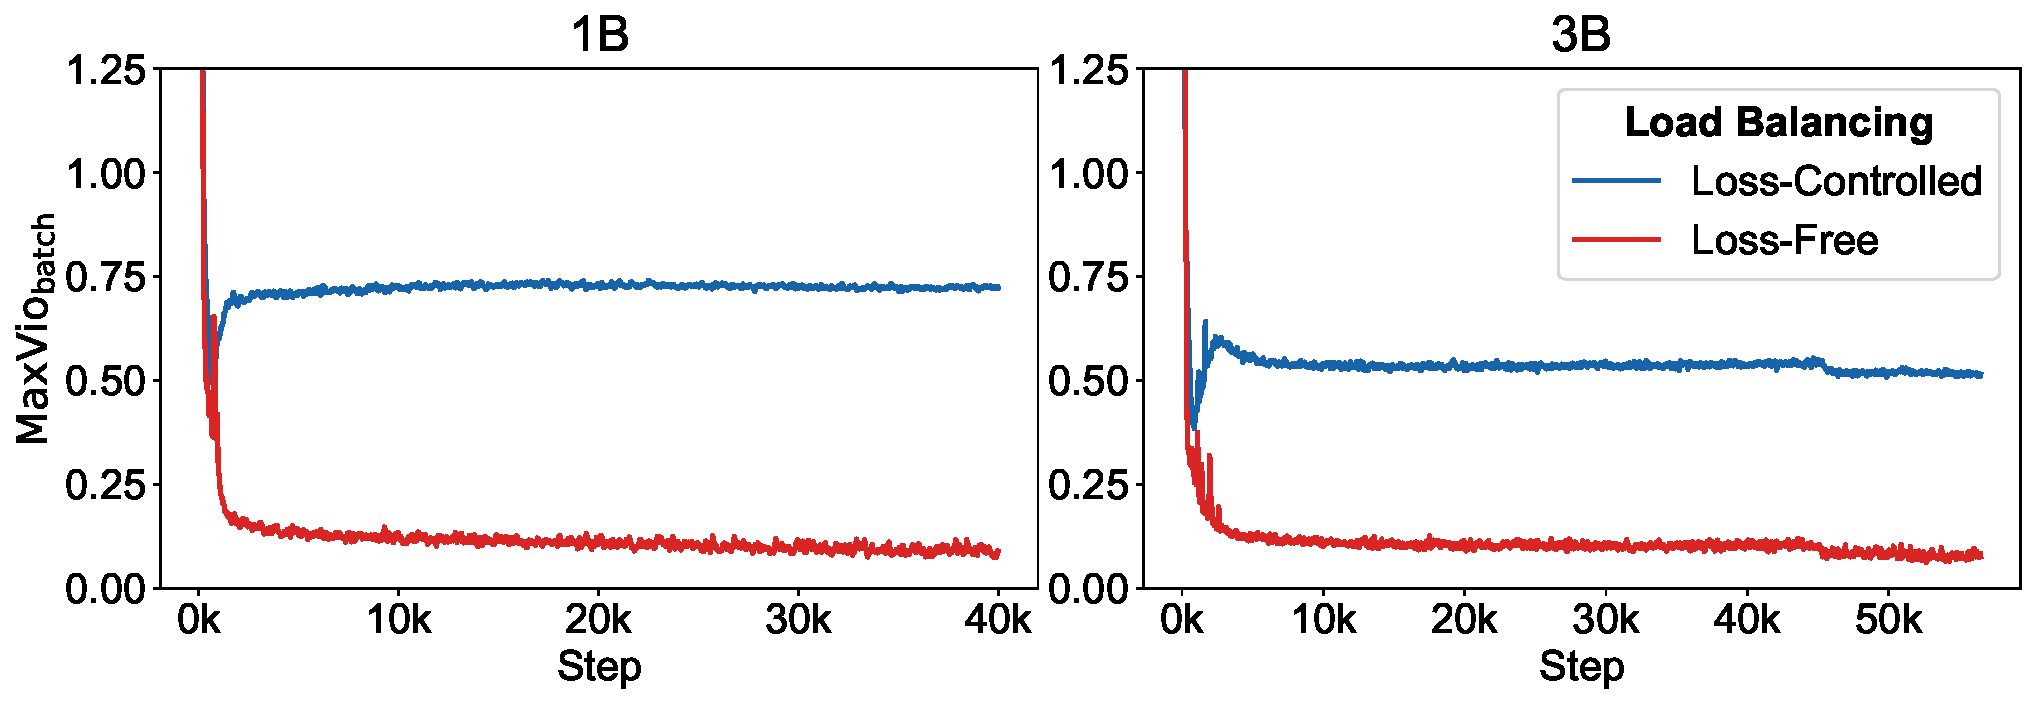
\includegraphics[width=1.0\textwidth]{figures/my_paper/update_rate_violations_main_avg100step_combined.pdf}
    \caption{训练过程中批次级负载均衡（MaxVio\textsubscript{batch}）的动态对比。}
    \label{fig:training_dynamics}
\end{figure}

\subsection{与专家并行（Expert Parallelism）的兼容性}
在训练超大规模混合专家模型时，通常会采用专家并行技术，即将不同的专家分布到不同的计算设备上。在这种设置下，计算批次（一次专家并行all-to-all涉及的数据，Computation Batch）内的负载均衡至关重要，因为它直接影响到设备间的通信开销和计算效率。

我们研究了无辅助损失均衡策略在不同计算批次大小下的表现。如图 \ref{fig:expert_parallelism_compatibility} 所示，随着计算批次大小的增加（这通常是专家并行度提高的结果），无辅助损失均衡策略的负载均衡效果会持续改善。相比之下，辅助损失方法的均衡效果在批次大小达到一定程度后便不再提升。这表明，\textbf{我们的无辅助损失均衡策略与专家并行天然兼容，并且在并行规模越大时，其优势越明显}。

\begin{figure}[h]
    \centering
    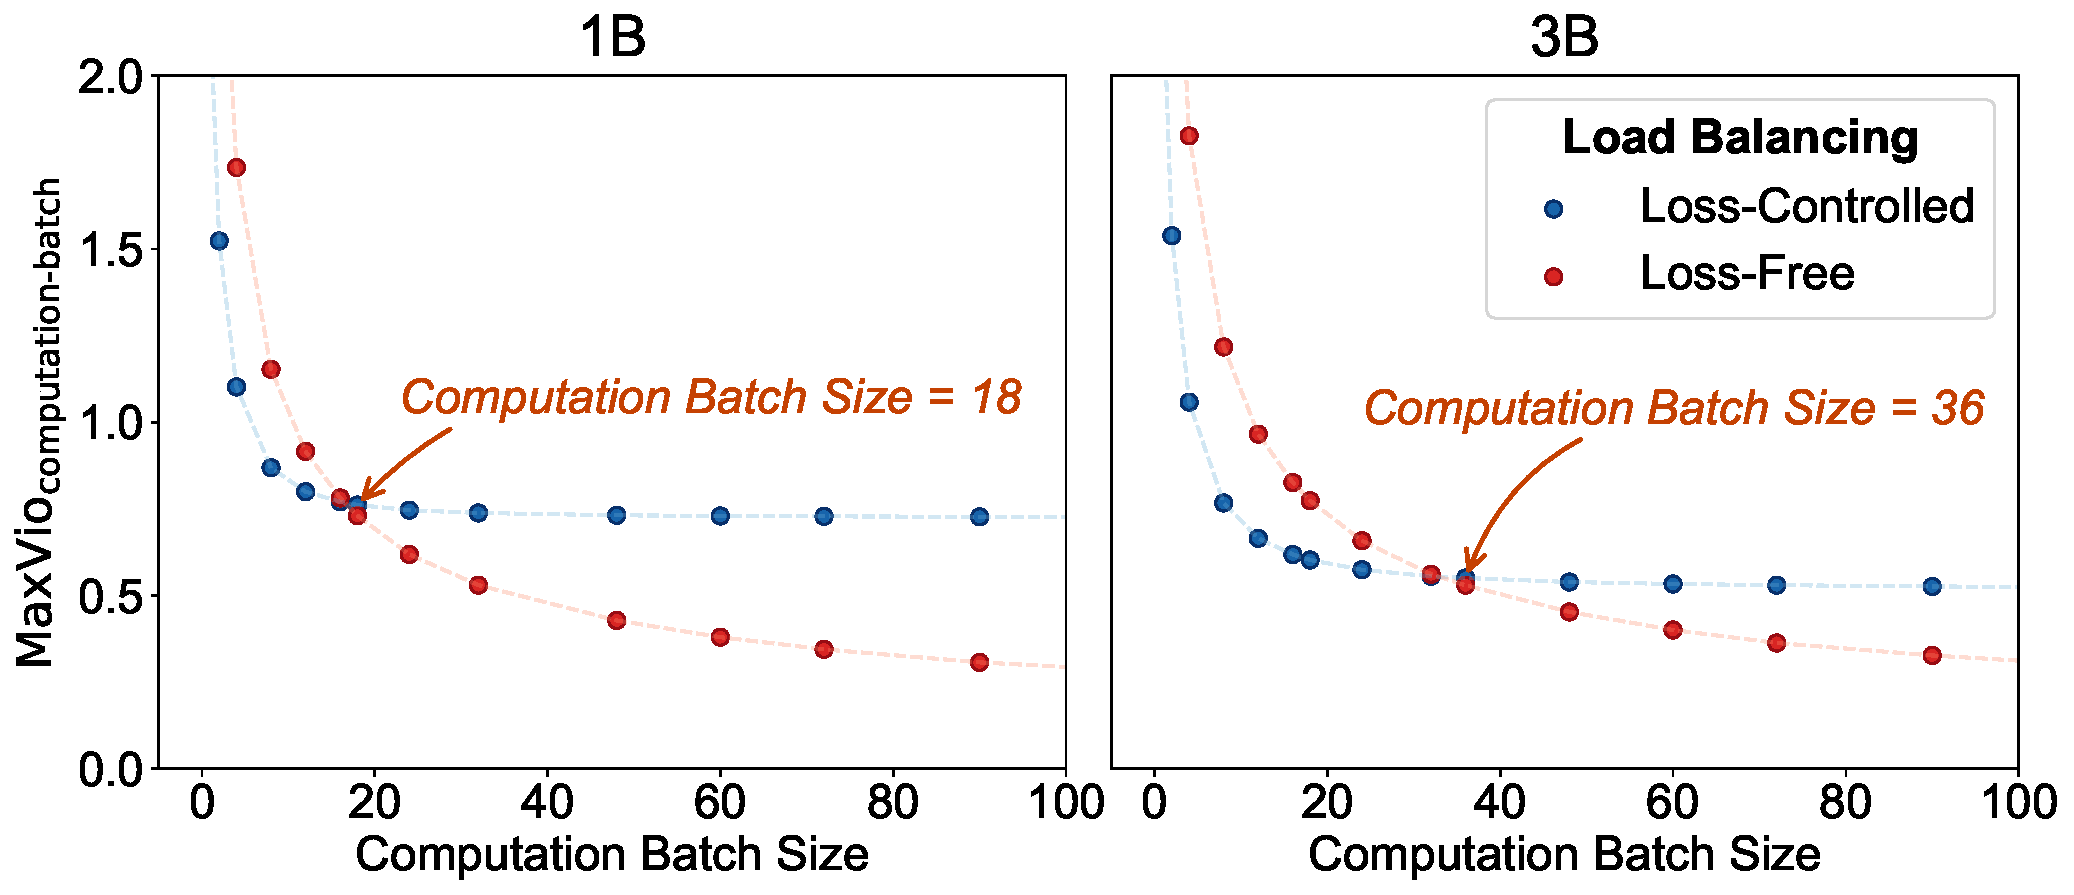
\includegraphics[width=1.0\textwidth]{figures/my_paper/actual_batch_violation_combined.pdf}
    \caption{随着计算批次大小增加，不同均衡策略的负载均衡表现。}
    \label{fig:expert_parallelism_compatibility}
\end{figure}

\subsection{与专家选择路由（Expert Choice Routing）的对比和未来词元泄露问题}
\label{sec:ec_leakage}
在负载均衡策略的探索中，除了主流的辅助损失函数方法，专家选择路由（Expert Choice Routing, EC）是另一种能够实现完美负载均衡的代表性方法\cite{Zhou2022MixtureofExpertsWE}。与传统方法中“词元选择专家”不同，专家选择路由的核心思想是“专家选择词元”：对于一个批次内的所有词元，每个专家会选择与自身亲和度最高的$k$个词元进行处理。通过设定一个全局统一的容量（capacity）$k$，可以保证每个专家处理完全相同数量的词元，从而从机制上消除了负载不均衡。

然而，专家选择路由存在一个与自回归语言模型根本原则相悖的严重问题：\textbf{未来词元泄露（Future Token Leakage）}\cite{Wang2024AuxiliaryLossFreeLB}。在标准的自回归模型训练中，模型在预测当前词元时，只能依赖于其之前的词元信息，这种因果约束（Causal Constraint）是模型泛化能力的基础。专家选择路由为了在整个词元序列（或一个计算块，chunk）中实现完美的负载均衡，其路由决策需要依赖该序列中的所有词元。这意味着，一个序列中较早位置的词元（例如$x_t$）的专家分配决策，会受到其后出现的词元（例如$x_{t+n}$）的影响（图\ref{fig:ec_leakage}）。

\begin{figure}[h]
    \centering
    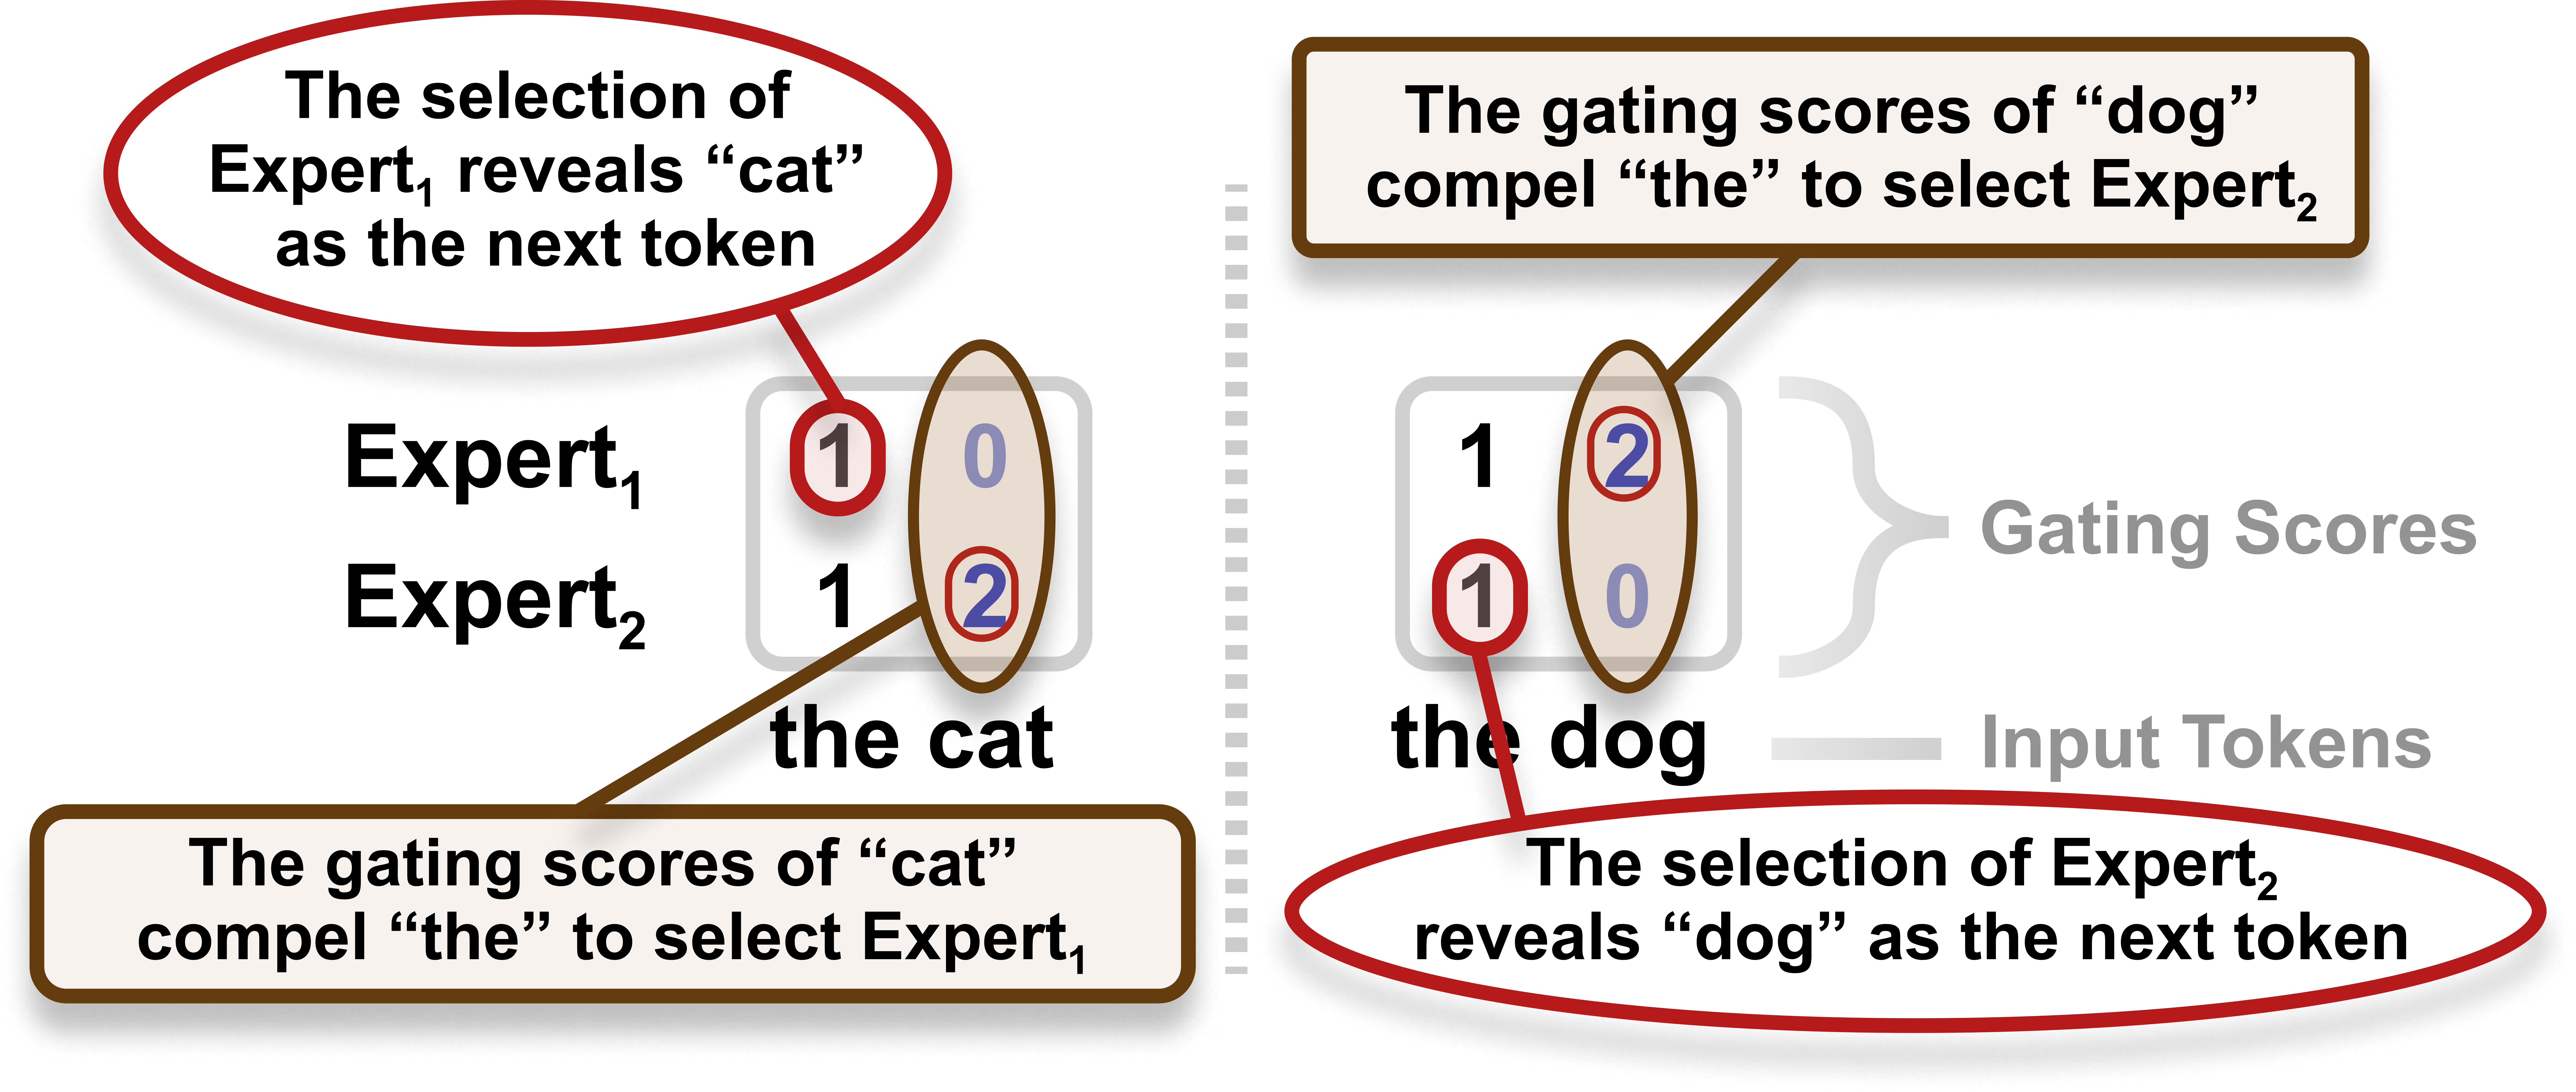
\includegraphics[width=1.0\textwidth]{figures/my_paper/EC_fig_new.png}
    \caption{后面的词元通过影响路由决策影响前面词元的混合专家模型层输出}
    \label{fig:ec_leakage}
\end{figure}

这种信息泄露是致命的，因为它使得模型在训练时可以“偷看”未来的信息来降低损失，影响了模型的正常学习，且使得训练损失失真（图\ref{fig:ec_leakage_curve}）。理论分析表明，对于一个稀疏率为$R$（即$K/N$，激活专家数除以总专家数）的混合专家模型层，EC路由每个词元最多可以泄露大约$K \log_2(\frac{1-R}{R})$比特的信息\cite{Wang2024AuxiliaryLossFreeLB}。在一个包含9个混合专家模型层、稀疏率为$1/8$（例如，从16个专家中选择2个）的典型模型中，泄露的信息总量（约50比特）足以让当前词元推断出下一个词元的身份。

\begin{figure}[h]
    \centering
    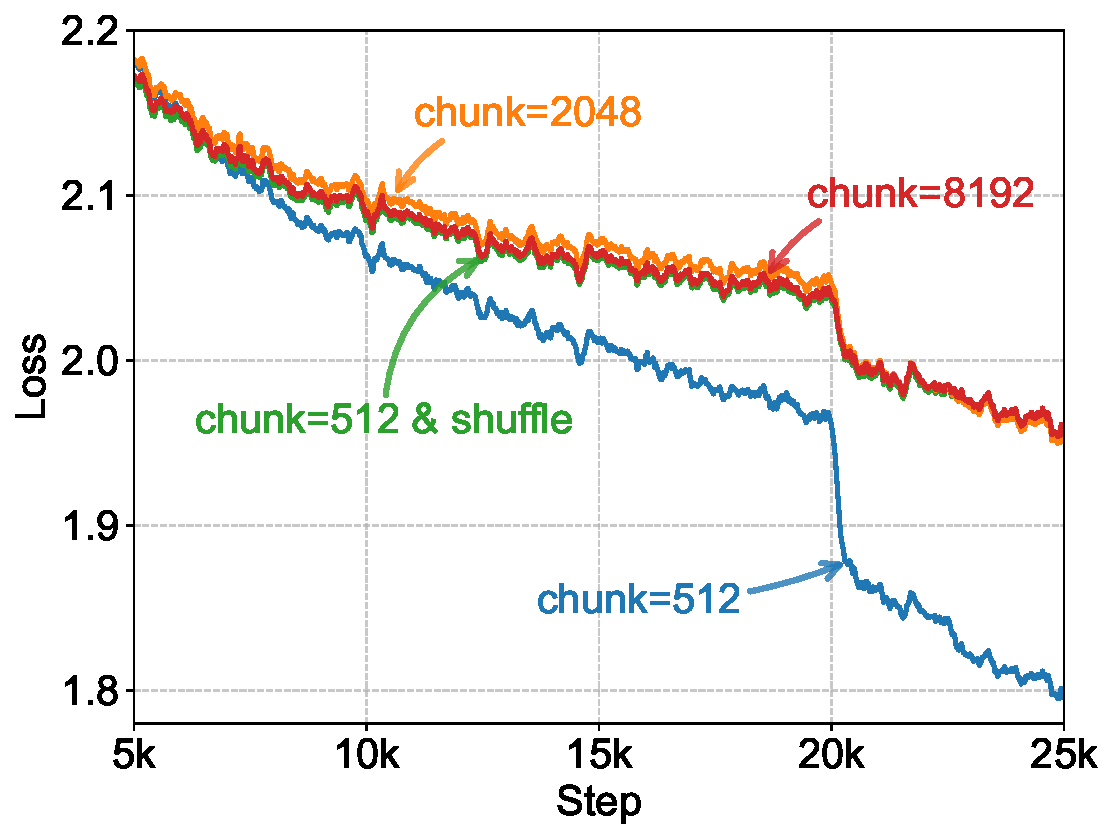
\includegraphics[width=0.7\textwidth]{figures/my_paper/ec_leakage.pdf}
    \caption{专家选择路由一次选择的范围（chunk）对训练损失的影响。范围越小，模型越容易利用信息泄露（图中蓝线），使训练损失异常降低；而打乱顺序则抑制了这种泄露（绿线）。}
    \label{fig:ec_leakage_curve}
\end{figure}

相比之下，我们提出的无辅助损失均衡策略通过基于历史批次的负载信息来更新偏置项，严格遵守了因果约束，不存在未来词元泄露的风险。这使得我们的方法在保证高效负载均衡的同时，能够更安全地应用于大规模自回归语言模型的训练。

\subsection{偏置更新算法的进一步研究}
\label{sec:bias_update_empirical}
为了验证我们在5.2.1节中提出的偏置项动态更新算法的有效性与最优配置，我们进行了一系列深入分析\cite{Wang2024AuxiliaryLossFreeLB}。研究主要围绕更新率、更新规则以及偏置形式这几个关键方面展开。

\paragraph{更新率（Update rate）的影响}
偏置项的更新率超参数$u$控制着偏置$b_i$收敛到“合适值”的速度。我们实验了不同的更新率设置，结果如图\ref{fig:update_rate_impact}所示。实验发现：
\begin{itemize}
    \item 一个过低的更新率（例如，$u=0.0001$）会导致偏置项收敛过慢。在训练初期，负载不均衡的问题得不到及时纠正。
    \item 一个过高的更新率（例如，$u=0.01$）虽然在初期能快速调整负载，但在训练后期，当负载已经趋于稳定时，过大的更新幅度反而会引入不必要的波动，破坏负载均衡的稳定性。
    \item 一个适中的更新率（例如，$u=0.001$）在收敛速度和后期稳定性之间取得了最佳平衡，能够在整个训练过程中保持良好且稳定的负载均衡效果，同时获得最优的模型性能（以困惑度衡量）。
\end{itemize}

\begin{figure}[h]
    \centering
    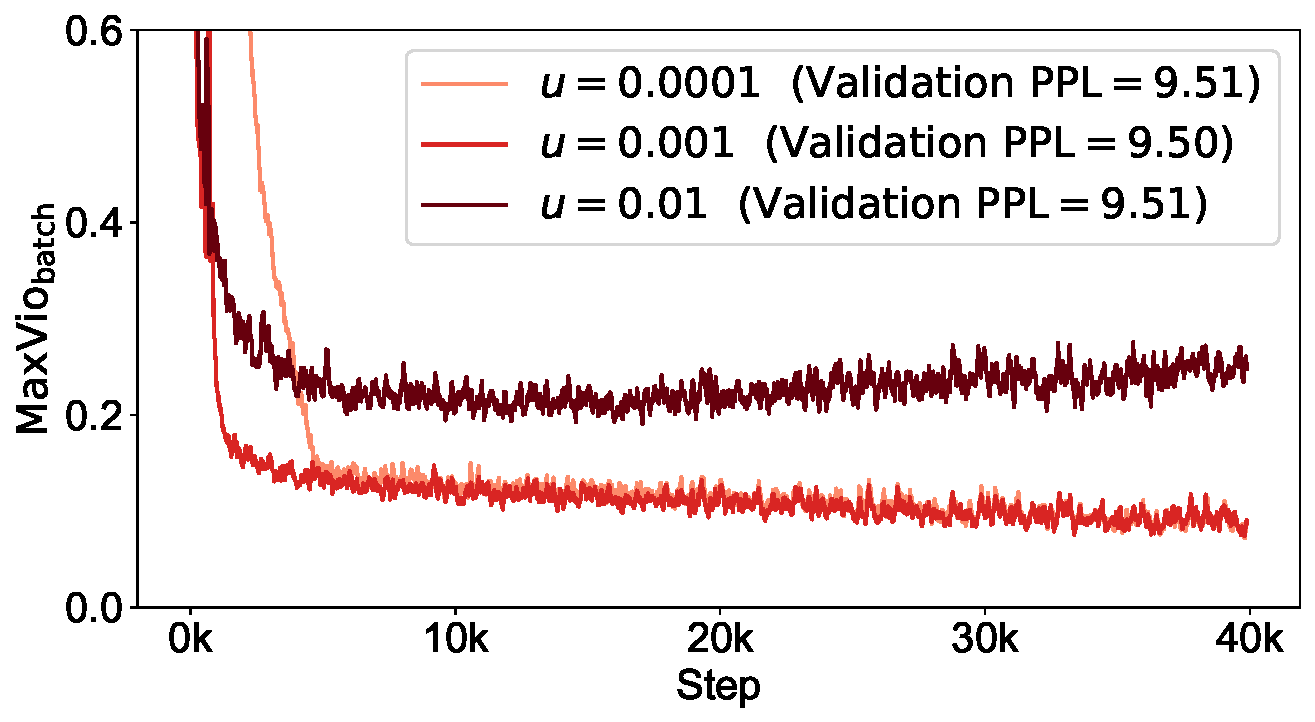
\includegraphics[width=0.7\textwidth]{figures/my_paper/update_rate_violations_avg100step.pdf}
    \caption{不同的更新率设置下，训练过程中的负载均衡}
    \label{fig:update_rate_impact}
\end{figure}

\paragraph{更新规则（Update rule）的比较}
我们使用的标准更新规则是基于负载违规误差$e_i$的符号，即 $b_i \leftarrow b_i + u \cdot \text{sign}(e_i)$。我们还研究了一种直接使用违规误差本身的变体规则：$b_i \leftarrow b_i + u \cdot e_i$。该规则旨在让负载偏差越大的专家，其偏置的调整幅度也越大。实验结果（见表\ref{tab:update_rule_comparison}）表明，尽管使用$e_i$直接更新能够在负载均衡指标上取得轻微优势，但并未带来模型最终性能的提升。考虑到符号更新规则的简洁性和鲁棒性，我们最终选择其作为标准算法。

\begin{table}[t]
\caption{不同更新规则的对比}
\label{tab:update_rule_comparison}
\begin{center}
\begin{tabular}{l|c|c}
\toprule
\multicolumn{1}{c|}{\textbf{Method}} & \textbf{Perplexity} & $\textbf{MaxVio}_\textbf{global}$ \\
\midrule
$b_i =  b_i + u*\text{sign}(e_i)$, $u=0.001$ & \textbf{9.50} & 0.044 \\
$b_i = b_i + u*e_i$, $u=0.01$ & 9.53 & \textbf{0.028}\\ 
$ b_i =  b_i + u*e_i$, $u=0.001$ &  9.51 & 0.036 \\
$ b_i = b_i + u*e_i$, $u=0.0001$ & 9.51  & 0.040 \\
\bottomrule
\end{tabular}
\end{center}
\end{table}

\paragraph{乘性偏置（Multiplicative bias）的可行性}
除了在我们路由分数上引入加性偏置（additive bias），我们还探索了使用乘性偏置（multiplicative bias）的可能性。即，路由决策由$\text{TopK}(\{s_{j,t} \cdot b_j|1\leq j\leq N\},K)$决定，其中偏置项$b_i$初始化为1。更新逻辑与加性偏置类似。实验对比（见表\ref{tab:multiplicative_bias_comparison}）发现，使用乘性偏置在负载均衡效果上与加性偏置相近，但会导致模型性能轻微下降。因此，我们最终确定加性偏置是更优越的选择。

\begin{table}[t]
\caption{加性偏置与乘性偏置的对比}
\label{tab:multiplicative_bias_comparison}
\begin{center}
\begin{tabular}{l|c|c}
\toprule
\multicolumn{1}{c|}{\textbf{Method}} & \textbf{Perplexity} & $\textbf{MaxVio}_\textbf{global}$ \\
\midrule
Addative Bias, $u=0.001$ & \textbf{9.50} & 0.044 \\
Multiplicative Bias, $u=0.01$ & 9.52 & 0.041 \\ 
Multiplicative Bias, $u=0.001$ &  9.52 & \textbf{0.036} \\
Multiplicative Bias, $u=0.0001$ & 9.54  & 0.048 \\
\bottomrule
\end{tabular}
\end{center}
\end{table}

\section{无辅助损失均衡策略的应用}
无辅助损失均衡策略作为一种简单、灵活、有效的混合专家模型负载均衡调控方法，已经在工业界得到了广泛应用。最近一年发布的国产开源大语言模型DeepSeek-V3~\cite{DeepSeekAI2024DeepSeekV3TR}，Kimi K2~\cite{Bai2025KimiKO}和GLM-4.5\cite{Zeng2025GLM45AR}均使用了这一方法。特别的，对于传统Top-K之外的场景，如不同专家计算量不同的情况，无辅助损失均衡策略也能高效的调控各个专家的负载乃至词元分配到的平均计算量。Grove MoE\cite{Wu2025GroveMT}使用它控制引入伴随专家情况下的负载均衡，而最近发布的大模型LongCat-Flash\cite{meituan-longcat_2025_longcat-flash-chat}也使用了这一策略来控制带零计算专家情况下的负载均衡。

\section{本章小结}
\label{sec:chapter_summary_personal}
本章详细介绍了我们在混合专家模型负载均衡方向的个人研究进展——一种无需辅助损失的无辅助损失均衡策略（Auxiliary-Loss-Free Balancing）。该策略通过引入并动态更新一个专家级的偏置项，直接在路由选择阶段主动引导负载均衡，从而避免了传统辅助损失方法所带来的“性能-均衡”困境。

我们的主要贡献包括：
\begin{enumerate}
    \item \textbf{提出了一个新的负载均衡框架}：该框架不依赖于损失函数和梯度，从根本上消除了对主任务训练的干扰。
    \item \textbf{设计了简洁有效的算法}：通过简单的偏置更新规则，实现了强大而稳定的负载控制。
    \item \textbf{进行了充分的实验验证}：在不同规模的模型上证明了该策略相比传统方法，在模型性能和负载均衡两方面均取得显著优势。
    \item \textbf{分析了其优势和兼容性}：阐明了其在避免信息泄露和与大规模并行训练兼容性方面的优点。
\end{enumerate}

这项研究为解决混合专家模型训练中的一个核心挑战提供了新的思路和有效的工具，对大规模、高效的稀疏模型研发具有重要的实践意义。
        % \chapter{当前研究进展及未来研究计划}
\label{chap:conclusion}

\section{总结}
\label{sec:summary}

    
    
    \appendix
    \printbibliography[heading = bibintoc]
    % 如有需要使用研究生成果页
    % \include{chap/ach}

	\backmatter
	% \include{chap/ack}
	% 需替换门户原创页pdf/扫描pdf
	% \include{chap/origin}

\end{document}

% vim:ts=4:sw=4